\documentclass{llncs}

\usepackage{amsmath}
\usepackage{amsfonts}
\usepackage{listings}
\usepackage[usenames,dvipsnames]{color}
\usepackage{alltt}
\usepackage{xspace}
\usepackage{multirow}
\pagestyle{plain}
\usepackage{xcolor}
\usepackage{algorithm2e}
\usepackage{tikz,pgfplots}
\usepackage{etoolbox}
\usepackage{mathtools}
\usepackage{caption}
%\usepackage{subcaption}
\usepackage{wrapfig}
\usepackage{listings}
%\usepackage{adjustbox}
%\usetikzlibrary{arrows,calc}
\captionsetup{compatibility=false}
%\usepackage{a4wide}
%\usepackage[margin=40mm, top=35mm]{geometry}

%\usepackage{latexsym}
\usepackage{setspace}
\usepackage{cancel}
\usepackage{graphicx}
\usepackage{appendix}
\usepackage{amssymb}
%\usepackage{times}

\usepackage{fancyvrb}
\usepackage[framemethod=tikZ]{mdframed}

%here are alternatives for the times package 
%%%%%%%%%%%%%%%%%%%%%%%%%%%%%%%
%\usepackage{times}
%-------
%\usepackage{pslatex}
%-------
\usepackage{mathptmx}
\usepackage{mathptm}
%-------
%\usepackage{mathtools}
%\usepackage{newtxmath} 
%\usepackage{newtxtext}
%%%%%%%%%%%%%%%%%%%%%%%%%%%%%%%
% \usepackage{fullpage}

%\usepackage{cancel}
%\usepackage{verbatim}
%\usepackage{chngpage}
%\usepackage{xcolor}
%\usepackage{mathrsfs}


\lstset{language=Java,
	basicstyle=\ttfamily\footnotesize,
	showspaces=false,
	showtabs=false,
	breaklines=true,
	showstringspaces=false,
	breakatwhitespace=true,
	commentstyle=\color{pgreen},
	keywordstyle=\color{blue},
	stringstyle=\color{red},
	basicstyle=\ttfamily
}

\newcommand{\Var}{\mathtt{Var}}
\newcommand{\Exp}{\mathtt{Exp}}
\newcommand{\Cmd}{\mathtt{Cmd}}
\newcommand{\Grd}{\mathtt{Grd}}
\newcommand{\Prg}{\mathtt{Prg}}
\DontPrintSemicolon
\SetKwRepeat{Loop}{Loop\{}{\}}%


\newcommand{\true}{\mathsf{true}}
\newcommand{\false}{\mathsf{false}}

\newcommand{\todo}[1]{{\color{blue}TODO:#1}}
\newcommand{\hide}[1]{}
\newcommand{\defn}{\overset{\triangle}{=}}
\newcommand{\maxi}{m}
\newcommand{\cur}{cur()}
\newcommand{\dom}[1]{\mathsf{dom}(#1)}
\newcommand{\ite}[3]{
	 \ifmmode
	 \mathbf{if}\ #1 \ \mathbf{then}\ #2\  \mathbf{else}\ #3
	 \else
	 \textbf{if}\ #1 \ \textbf{then}\ #2\  \textbf{else}\ #3
	 \fi}
\newcommand{\rloop}{
	\ifmmode
	\mathbf{Loop}
	\else
	\textbf{Loop}
	\fi}

\newcommand{\Z}{\mathbb{Z}}

\title{\hspace{-0.1cm}{J-ReCoVer}:~Java~Reducer~Commutativity~Verifier}
\author{}
\institute{}
\hide{
\author{
Yu-Fang Chen\inst{1}\inst{2}
\and
Chang-Yi Chiang\inst{2}
\and
Hsin-Hung Lin\inst{1}
\and
Wei-Tsung Kao\inst{1}
\and
Yean-Fu Wen\inst{2}
\and
Wei-Cheng Wu\inst{1}
}
\institute
{
Institute of Information Science, Academia Sinica, Taiwan
\and
Graduate Institute of Information Management, National Taipei University, Taiwan
}}
\author{}
\institute{}

%%%%%%%%%%%%%%%%%%%%%%%%%%%%%%%%%%%%%%%%%%%%%%%%%%%%%%%%%%%%%%%%%%%%%%%%%%%%%%
\begin{document}
%%%%%%%%%%%%%%%%%%%%%%%%%%%%%%%%%%%%%%%%%%%%%%%%%%%%%%%%%%%%%%%%%%%%%%%%%%%%%%

\maketitle

\begin{abstract}

The MapReduce framework for data-parallel computation was first proposed by
Google~\cite{dean04} and later implemented in the Apache Hadoop
project~\cite{hadoop}. Under the MapReduce framework, a reducer computes output
values from a sequence of input values transmitted over the network. Due to
non-determinism in data transmission, the order in which input values arrive at
the reducer is not fixed. In relation to this, the \emph{commutativity problem}
of reducers asks if the output of a reducer is independent of the order of its
inputs. Indeed, there are several advantages for a reducer to be commutative,
e.g., the verification problem of a MapReduce program can be reduced to the
problem of verifying a sequential program. We present the tool J-ReCoVer (Java
Reducer Commutativity Verifier) that implements effective heuristics for reducer
commutativity analysis. J-ReCoVer is the first tool that is specialized in
checking reducer commutativity. Our experimental results over 118 benchmark
examples collected from open repositories are very positive; J-ReCoVer correctly
handles over 97~\% of them.

\end{abstract}

%%%%%%%%%%%%%%%%%%%%%%%%%%%%%%%%%%%%%%%%%%%%%%%%%%%%%%%%%%%%%%%%%%%%%%%%%%%%%%
\section{Introduction} \label{section:introduction}
%%%%%%%%%%%%%%%%%%%%%%%%%%%%%%%%%%%%%%%%%%%%%%%%%%%%%%%%%%%%%%%%%%%%%%%%%%%%%%

MapReduce belongs among the most popular frameworks for data parallel
computation. A MapReduce program~\cite{dean04,hadoop} consists of several pairs
of \emph{mappers} and \emph{reducers} running on a machine cluster for handling
big data in parallel. Usually, mappers and reducers are the only components in a
MapReduce program that involve concurrency. Mappers read data from a distributed
database and output a sequence of \emph{key-value} pairs. The elements of the
sequence (i.e., key-value pairs) with the same key are sent to the same reducer
for further processing. Due to scheduling policies and network latency, the same
inputs may arrive at a reducer in different orders in different executions.
Therefore, reducers are typically required to be \emph{commutative}, that is,
the output of a reducer is required to be independent of the order of its
inputs. The problem of checking whether this is indeed the case is known as the
\emph{commutativity problem} of
reducers~\cite{csallner13testing,xiao14mr,ChenHSW15,ChenSW16}. If all reducers
are commutative, they will have the same external behavior under all possible
schedules. In such a case, by fixing a schedule, the verification problem of a
MapReduce program can be reduced to the verification problem of a sequential
program, which is known to be much easier than the verification problem of
concurrent programs. One then suffices with considering any chosen interleaving
of input values instead of all of them.

% More concretely, for the verification of a MapReduce program, we propose to do
% it in two phases. First, ensuring if all reducers are commutative. If some
% reducers are non-commutative, modifying them to commutative ones. Usually, the
% modification is not a difficult task~\cite{xiao14mr}, and can be done without
% affecting their functionality and performance. For example, assume that the
% task of a reducer is to find the name of the person with highest score. Such a
% reducer is non-commutative when the input include two people with the same
% highest score. This reducer can be made commutative, by also comparing the ID
% number of people with the same score. Once all reducers are made commutative,
% we reduce the verification problem to sequential verification by fixing a
% scheduler. In this two-phase approach, the key enabling technique is an
% efficient procedure for checking reducer commutativity.

On the other hand, the non-commutative behavior of a reducer is often the source
of very tricky bugs. A study conducted by Microsoft investigated the
commutativity problem of $508$ reducers running on their MapReduce
server~\cite{xiao14mr}. These reducers were carefully checked using all
traditional means such as code review, testing, and experiments with real data
for months. Still, five of these programs contained very subtle bugs caused by
non-commutativity (which was confirmed by the programmers).

However, checking reducer commutativity is a difficult problem on its own
right~\cite{ChenHSW15,ChenSW16,ChenLTW17}. Even for a simple case in which all
values are mathematical integers, it is proved undecidable in~\cite{ChenHSW15}.
For the case when all values are machine integers (e.g., 64-bits integers), the
problem is decidable, but the only available algorithm, which was proposed
in~\cite{ChenHSW15} too, is of very high complexity and hence of theoretical
interest only.

In this paper, we present the J-ReCoVer tool (Java Reducer Commutativity
Verifier), which is available at~\verb|http://jrecover.iis.sinica.edu.tw|. The
tool implements a heuristic approach for checking the commutativity problem
that---despite its simplicity---works very efficiently on a large set of
practical integer reducer programs as shown by our experiments. The main
ingredient of the approach is a reduction from the commutativity problem to an
SMT problem. The reduction is incomplete but sound. It is accompanied with
several heuristics which enable the approach to scale to real-world examples.
For the case when the reducer is not proven commutative, we complement the
approach by using testing to find concrete counterexamples.

We collected benchmarks from open repositories such as Github and Bitbucket to
evaluate J-ReCoVer. With the help of a search engine \emph{searchcode.com} over
those repositories, we collected 118 programs. We provide this collection of
programs to other interested researchers as a side contribution of the paper.
Our tool J-ReCoVer is able to correctly analyze all but three of the programs.

%=============================================================================
\subsection*{Related Works}
%=============================================================================

The reducer commutativity problem can be reduced to a \emph{program equivalence}
problem. One creates another program $R'$ that first non-deterministically swaps
two consecutive input values and then executes the code of $R$. If $R'$ and $R$
are equivalent, using the fact that all permutations of a list can be obtained
by swapping consecutive list elements finitely many times\footnote{Here is an
example to produce [3;2;5;1;4] from [1;2;3;4;5] by swapping consecutive
elements: [\textbf{1};\textbf{2};3;4;5] $\rightarrow$
[2;\textbf{1};\textbf{3};4;5] $\rightarrow$
[2;3;1;\textbf{4};\textbf{5}]$\rightarrow$
[2;3;\textbf{1};\textbf{5};4]$\rightarrow$
[\textbf{2};\textbf{3};5;1;4]$\rightarrow$ [3;2;5;1;4].}, $R$ can be proved to
be commutative. There is a series of research results on program equivalence
checking (or closely related topics such as regression verification and
translation validation): see, e.g.,
\cite{Pnueli:1998:TV,fedyukovich2015automated,barthe2011relational,KlebanovRuemmerUlbrich2017}
to name a few. 

From a high-level view, checking equivalence of two programs $P$ and $P'$ can be
reduced to a sequential verification problem by executing $P'$ after $P$,
followed by checking whether the two programs always produce the same outputs.
The approach can be made more efficient by finding the
right~\emph{synchronization points} and combining the code of $P$ and $P'$ in an
interleaved manner. A lot of research effort in this direction is in finding
good synchronization points. In this work, we propose the \emph{head of the
top-level reducer loop} as the synchronization point suitable for reducer
commutativity analysis. According to our experience discussed later on, the
reducers usually contain just a single such loop. Moreover, for the case when
there are more top-level loops in a reducer, we propose a way of breaking such a
reducer into several ones to be checked independently.

However, in our experience, if one naively reduces the commutativity problem to
an equivalence problem and checks it in a precise manner, many reducers cannot
be verified. Therefore, J-ReCoVer uses an over-approximation of the reducer's
behavior. This approximation allows for a much more efficient, yet---according
to our experiments---precise enough commutativity analysis.

Our approach can be seen as using some form of \emph{sequentialisation} of the
concurrent behaviour. Sequentialisation is the key approach behind many current
successful approaches for verifying multithreaded
programs~\cite{LalReps:Seq:08,LazyCSeq14}. However, our sequentialisation
approach is specialised for the case of reducers and quite different from what
is used in sequentialisation of multithreaded programs: indeed, in MapReduce
programs there is no notion of threads nor context switches.

Various forms of sequentialisation are behind further research works too, such
as, e.g., works dealing with the concept of \emph{robustness} of event-driven
asynchronous programs~\cite{ahmed2017:robustness} or those dealing with programs
running under some \emph{relaxed memory
models}~\cite{ahmed2013:robustness,AbdullaACLR13,AbdullaACLR12}. However, their
computation models are again quite different from that of reducers, and hence
the results cannot be directly applied.
Besides verification, another interesting research direction is the
\emph{synthesis} of MapReduce programs~\cite{SmithA16}. Commutativity analysis
is used as a component under the synthesis framework.

%%%%%%%%%%%%%%%%%%%%%%%%%%%%%%%%%%%%%%%%%%%%%%%%%%%%%%%%%%%%%%%%%%%%%%%%%%%%%%
\section{Notations and Definitions} \label{section:integer-reducers}
%%%%%%%%%%%%%%%%%%%%%%%%%%%%%%%%%%%%%%%%%%%%%%%%%%%%%%%%%%%%%%%%%%%%%%%%%%%%%%

We use $[n,m]$ to denote the set of integers $\{k\mid n \leq k\leq m\}$ and lift
the equality $=$ operation to tuples in the standard way.

% \begin{equation*}
% \begin{array}{rclcl}
% \multicolumn{3}{l}{v\in \Var\mbox{, and }c \in \Z}&&\textmd{Variable and 
%   Constant}\\
% e \in \Exp    &\ \ \  {\triangleq}\ \ \   & v \mid c \mid \cur \mid e + e \mid
%   e - e \mid e \times e \mid *\mid\ldots & &\textmd{Integer Expression}\\
% g\in \Grd  & {\triangleq}  & e < e \mid not\ g \mid g \wedge g  \mid \ldots& & 
%   \textmd{Guard}\\
% s\in \Cmd  & {\triangleq}  & v:= e \mid out(v) \mid \ite{g}{s}{s} \mid s;s && 
%   \textmd{Command}\\
% p\in \Prg  & {\triangleq}  & s;\rloop\{s\};s&& \textmd{Reducer Program}\\
% \end{array}
% \end{equation*}

\begin{wrapfigure}{r}{3cm}
		\vspace{-0.8cm}

%		\begin{minipage}{0.32\textwidth}
%			\begin{algorithm}[H]
%				$m := \cur$; \;
%				\Loop{}{
%					$t:=\cur$;\;
%					\uIf{ $t > m$}{
%						$m := t$
%					}
%				};
%				$out(m)$\;
%			\end{algorithm}
%			\caption*{(a) max}
%		\end{minipage}
%		\hspace{-0.5cm}
	
	\begin{minipage}{0.3\textwidth}
		\begin{algorithm}[H]
			$s := 0;c:=0$; \;
			\Loop{}{
				$s := s+\cur$;\;
				$c := c+1$
			};
			$o := s/c$;\;
			$out(o)$\;
		\end{algorithm}
	\end{minipage}

% 		\begin{minipage}{0.4\textwidth}
% 			\begin{algorithm}[H]
% 				$a:=*;s := 0; c:=0$;\;
% 				\Loop{}{
% 					$s := s+(\cur-a)^2$; \;
% 					$c := c+1$
% 				};
% 				$o := s/c$;\;
% 				$out(o)$
% 			\end{algorithm}
% 			\caption*{(c) standard deviation}
% 		\end{minipage}

	\caption{A reducer that computes the average value.}
	\vspace{-0.8cm}
	\label{fig:reducer_example}
\end{wrapfigure}

For presentation purposes, we provide a sketch of a highly simplified language
for describing reducers. The language allows us to give examples of reducers and
to discuss our approach for checking their commutativity. Let $\Var$ be a set of
\emph{integer variables}. An \emph{integer expression} in $\Exp$ can either be
a~variable from $\Var$, a constant value, a call to the $\cur$ function that
reads and consumes an input value of the reducer, their combinations over basic
arithmetic operations, or a non-deterministically chosen integer value $*$. A
\emph{command} in $\Cmd$ can be an assignment, a branch statement, a sequence of
commands, or an $out(v)$ statement that outputs the value of $v \in \Var$. A
\emph{reducer program} is defined as $s_1;\rloop\{s_2\};s_3$ where $s_1,s_2,s_3
\in \Cmd$. According to our observation over hundreds  of reducer programs in
open repositories, reducer programs are almost always in this form. The
$\rloop\{s_2\}$ statement enters the loop body to execute $s_2$ repeatedly until
the entire input list is consumed. An example of a reducer is shown in
Figure~\ref{fig:reducer_example}.

Some reducers use two (or more) top-level loops to compute the output, possibly
interleaved with some non-looping code. These loops are executed sequentially,
repeatedly iterating over the input list from its beginning. For example, for
calculating the standard deviation, one first computes the average of inputs and
then uses it to compute the final result (using two passes over the input list).
In that case, we suggest to verify the reducer by first partitioning it into two
(or more) reducers, each containing a single top-level loop, and then verifying
these reducers separately.\footnote{Nested loops can be removed by adding
additional branch statements since both the inner and outer loop are over the
same input list. In fact, such a program construct has never occurred in the
examples we have seen.} The top-level loops communicate through shared
variables. After the transformation, reducers corresponding to the second
top-level loop (and possibly further such loops) will work with random initial
values of the shared variable, which over-approximates the original behavior.
Usually, the second (or further) top-level loop are commutative even with
arbitrary initial shared variable values and hence J-ReCoVer can be used to
prove it.

%For instance, for the case of the standard deviation, the first reducer computes
%the average, and the other reducer performs the rest of the computation. The
%second reducer replaces the average with a non-deterministic value and thus
%``over-approximates'' all possible outputs of the standard deviation
%computation. Equivalently, it computes an output for all possible ``average''
%values. However, this reducer is still commutative, and its commutativity can be verified.

%%%%%%%%%%%%%%%%%%%%%%%%%%%%%%%%%%%%%%%%%%%%%%%%%%%%%%%%%%%%%%%%%%%%%%%%%%%%%%
\vspace*{-2mm}
\section{Overview of the J-ReCoVer Tool} \label{sec:overview}
\vspace*{-1mm}
%%%%%%%%%%%%%%%%%%%%%%%%%%%%%%%%%%%%%%%%%%%%%%%%%%%%%%%%%%%%%%%%%%%%%%%%%%%%%%

%Hadoop, Java;

The input of J-ReCoVer is a reducer program written in Java, which is the most
popular programming language used in the Hadoop~\cite{hadoop} MapReduce
framework. The J-ReCoVer tool has three main components, the
\emph{Preprocessor}, the \emph{Prover}, and the \emph{BugFinder}. As the name
suggests, the Preprocessor reads as input a reducer program and performs the
required preprocessing. The goal of Prover is to show that a given reducer is
commutative, and the goal of BugFinder is the opposite. The architecture of
J-ReCoVer can be found in Figure~\ref{fig:overview-jrecover}. The user can input
a reducer program to J-ReCoVer either through our web-interface or use a binary
application installed on his/her own machine.

The \emph{Preprocessor component} first compiles a reducer program to bytecode
and uses the tool Soot to further convert it to the so-called ``Jimple'' format,
which is an intermediate language designed to simplify the analysis of Java
programs. Under the Hadoop MapReduce framework, the permutation of the input is
handled by the scheduler/shuffler component and is affected by issues like
network latency, which are not controllable by programmers. In order to deal
with such issues, we wrote our own dummy Hadoop environment for the reducer as a
part of the Preprocessor component so that the input order of the reducer is now
controlled by J-ReCoVer. Finally, the Preprocessor performs some program
transformation tasks to simplify the analysis. For example, it converts all
output commands $out(e)$ inside loops to a special assignment (as explained in
Section~\ref{sec:program_trans1}).

\begin{wrapfigure}{r}{7cm}
	\vspace{-8mm}
\centering
	\scalebox{0.7}{
		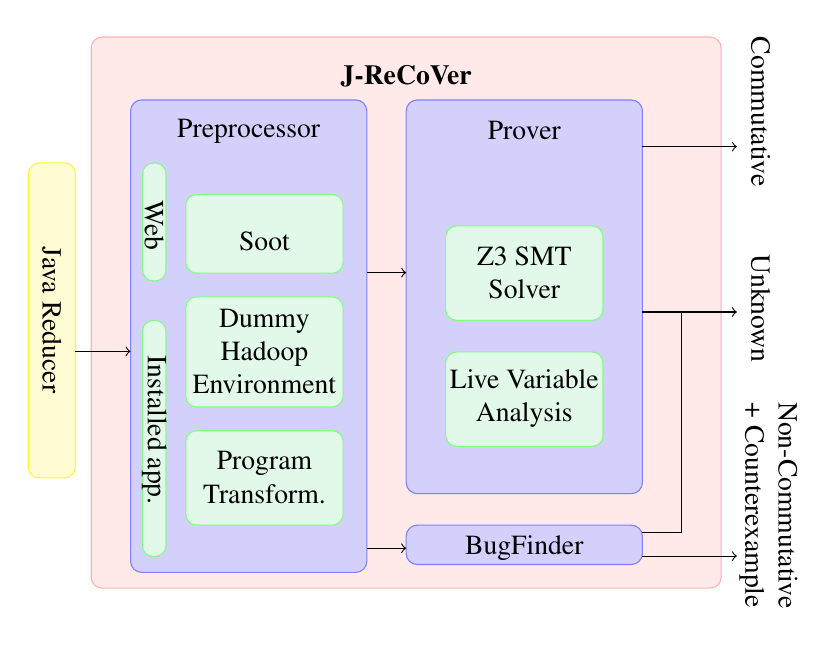
\begin{tikzpicture}


		%J-ReCoVer
		\node[draw=red!30, inner sep=0, anchor=north,rounded corners, fill opacity=0.85,text width=8cm,fill=red!10,minimum height=7cm] (jrecover) at (5,0) {};
		\node at (5,-.5) {\textbf{J-ReCoVer}};

		%JAVA reducer
		\node[draw=yellow!80, inner sep=0, anchor=north,rounded corners, fill opacity=0.85,text width=0.6cm,fill=yellow!20,minimum height=4cm] (reducer) at (0.5,-1.6) {};
		\node[rotate=270, align = center] at (0.5,-3.6) {Java Reducer};


		%JPreprocessor
		\node[draw=blue!50, inner sep=0, anchor=north,rounded corners, fill opacity=0.85,text width=3cm,fill=blue!20,minimum height=6.cm] (preprocessor) at (3,-.8) {};
		\node[] at (3,-1.2) {Preprocessor};

		%JPreprocessor->Interface
		\node[draw=green!50, inner sep=0, anchor=north,rounded corners, fill opacity=0.85,text width=0.3cm,fill=green!10,minimum height=1.5cm] (interface1) at (1.8,-1.6) {};
		\node[rotate=270, align = center] at (1.8,-2.4) {Web};

		\node[draw=green!50, inner sep=0, anchor=north,rounded corners, fill opacity=0.85,text width=0.3cm,fill=green!10,minimum height=3cm] (interace2) at (1.8,-3.6) {};
		\node[rotate=270, align = center] at (1.8,-5) {Installed app.};

		%JPreprocessor->Technologies
		\node[draw=green!50, inner sep=0, anchor=north,rounded corners, fill opacity=0.85,text width=2cm,fill=green!10,minimum height=1cm] (soot) at (3.2,-2) {};
		\node at (3.2,-2.6) {Soot};

		\node[draw=green!50, inner sep=0, anchor=north,rounded corners, fill opacity=0.85,text width=2cm,fill=green!10,minimum height=1.4cm] (symex) at (3.2,-3.3) {};
		\node at (3.2,-4) {
			\begin{minipage}[t]{0.222\textwidth}
			\centering
			Dummy\\
			Hadoop\\
			Environment
			\end{minipage}		
			};

			\node[draw=green!50, inner sep=0, anchor=north,rounded corners, fill opacity=0.85,text width=2cm,fill=green!10,minimum height=1.2cm] (prog_trans) at (3.2,-5) {};
			\node at (3.2,-5.6) {
				\begin{minipage}[t]{0.222\textwidth}
				\centering
				Program\\
				Transform.
				\end{minipage}
			};

		%JProver
		\node[draw=blue!50, inner sep=0, anchor=north,rounded corners, fill opacity=0.85,text width=3cm,fill=blue!20,minimum height=5cm] (prover) at (6.5,-0.8) {};
		\node[] at (6.5,-1.2) {Prover};

		%JProver->Technologies
		\node[draw=green!50, inner sep=0, anchor=north,rounded corners, fill opacity=0.85,text width=2cm,fill=green!10,minimum height=1.2cm] (z3) at (6.5,-2.4) {};

		\node at (6.5,-3) {
			\begin{minipage}[t]{0.222\textwidth}
			\centering
			Z3 SMT \\
			Solver
			\end{minipage}
		};


		\node[draw=green!50, inner sep=0, anchor=north,rounded corners, fill opacity=0.85,text width=2cm,fill=green!10,minimum height=1.2cm] (z3) at (6.5,-4.) {};

		\node at (6.5,-4.6) {
			\begin{minipage}[t]{0.222\textwidth}
			\centering
			Live Variable \\
			Analysis
			\end{minipage}
		};

		%JBugFinder
		\node[draw=blue!50, inner sep=0, anchor=north,rounded corners, fill opacity=0.85,text width=3cm,fill=blue!20,minimum height=0.5cm] (learner) at (6.5,-6.2) {};
		\node[] at (6.5,-6.5) {BugFinder};


		%JResults


		\node[rotate=270, align = center] at (9.5,-1) {
			Commutative
		};

		\node[rotate=270, align = center] at (9.5,-3.5) {
			Unknown
		};

		\node[rotate=270, align = center] at (9.6,-6) {
			\begin{minipage}[t]{0.25\textwidth}
			\centering
			Non-Commutative	 \\
			+ Counterexample
			\end{minipage}

		};


		\draw [->] (8,-6.6) -- (9.2,-6.6) ;
		\draw [->] (8,-1.4) -- (9.2,-1.4) ;
		\draw [-] (8,-6.3) -- (8.5,-6.3) --(8.5,-3.5);
		\draw [->] (8,-3.5) -- (9.2,-3.5) ;

		\draw [->] (4.5,-3) -- (5,-3) ;
		\draw [->] (4.5,-6.5) -- (5,-6.5) ;

		\draw [->] (0.8,-4) -- (1.5,-4) ;

		\end{tikzpicture}
	}
		\vspace{-1cm}
	\caption{Overview of the J-ReCoVer Tool. }\label{fig:overview-jrecover}
		\vspace{-0.8cm}
	
\end{wrapfigure}

%!!!!!!!!!!!!!!!!!!!!!!!!!!!!!!!!!!!!
\enlargethispage{4mm}
%!!!!!!!!!!!!!!!!!!!!!!!!!!!!!!!!!!!!

The \emph{BugFinder component} randomly generates pairs of lists. The lists in a
pair are permutations of each other. A concrete counterexample is reported if
inputting any pair of lists from the generated ones to the reducer generates
different results. Our procedure for generating random pairs is quite naive. We
use five different input list of lengths 5, 7, 9, 11, and 13. For each length,
we generate 300 lists and pick uniformly at random one of its permutations.
Although the approach is simple; in practice, it finds counterexamples in all of
our non-commutative benchmarks in a few seconds. 

The \emph{Prover component} reduces the commutativity problem to an SMT
satisfiability problem. From a high-level point of view, we check equivalence
between a reducer program and its variant that has two consecutive inputs
swapped. We show that this can be reduced to a first-order formula and give it
to the SMT solver Z3 for solving. In case that Z3 proves the formula
unsatisfiable, we know that swapping any two consecutive inputs of the reducer
will not change its output. Since all permutations of a list can be obtained by
swapping consecutive elements finitely many times, it follows that the reducer
outputs the same value for all permutations of the same list of inputs. In this
case, J-ReCoVer stops and reports that the reducer is commutative.

%%%%%%%%%%%%%%%%%%%%%%%%%%%%%%%%%%%%%%%%%%%%%%%%%%%%%%%%%%%%%%%%%%%%%%%%%%%%%%
\vspace*{-2mm}
\section{The Preprocessor and the Prover} \label{sec:preprocessor_prover}
\vspace*{-1mm}
%%%%%%%%%%%%%%%%%%%%%%%%%%%%%%%%%%%%%%%%%%%%%%%%%%%%%%%%%%%%%%%%%%%%%%%%%%%%%%

Before entering the Prover component, the Preprocessor first performs two
program transformations to simplify the verification task
(Section~\ref{sec:program_trans1}). The output of the preprocessor is a
commutativity-equivalent reducer program. The algorithm of the Prover is then
explained in Section~\ref{sec:prover}. 

%=============================================================================
\vspace*{-2mm}
\subsection{The Program Transformations in the Preprocessor}
\label{sec:program_trans1}
\vspace*{-1mm}
%=============================================================================

%-----------------------------------------------------------------------------
\paragraph*{Handling the access to $\cur$ before entering the loop.}
%-----------------------------------------------------------------------------

\begin{wrapfigure}[11]{r}{3.5cm}
	\vspace{-17mm}
	\begin{algorithm}[H]
		\;\;$m := \cur + 10$; \;
		\Loop{}{
			$t:=\cur$\;
			\uIf{ $t> m$}{
				$m := t$ \;
			}
		};
		$out(m)$\;\;
	\end{algorithm}
	\vspace{-0.8cm}
	\caption{The max$^+$ reducer with input before the main loop.}
	\vspace{-12mm}
	\label{fig:reducer_max1}
\end{wrapfigure}	

%	\begin{figure}[t]
%		\begin{minipage}{0.4\textwidth}
%			\begin{algorithm}[H]
%				\;\;$m := \cur + 10$; \;
%				\Loop{}{
%					$t:=\cur$\;
%					\uIf{ $t> m$}{
%						$m := t$ \;
%					}
%				};
%				$out(m)$\;\;
%			\end{algorithm}
%			\caption*{(a) Reducer max$^+$}
%		\end{minipage}
%		\begin{minipage}{0.6\textwidth}
%			\begin{algorithm}[H]
%				$s:=*;$\;
%				\Loop{}{
%					\uIf{$s=1$}{$m := \cur + 10; s:= 2$}
%					\uElse{
%						$t:=\cur$\;
%						\uIf{ $t > m$}{
%							$m := t$ \;
%						}
%					}
%				};
%				$out(m)$
%			\end{algorithm}
%			\caption*{(b) Reducer max$^{+\mathtt{fix}}$}
%		\end{minipage}
%		\caption{Reducer examples}
%		\label{fig:reducer_max}
%	\end{figure}

In real-world reducers, it is often the case that the $s_1$ part of the reducer
reads from the input. Since our reduction of the commutativity problem to SMT
solving, which is presented in Section~\ref{sec:prover}, concentrates on the
influence of the input on the loop $s_2$ only, we need to transform the reducer
such that any input happens in the loop only. 

In order to be able to explain the transformation that we perform on an example,
consider the example in Figure~\ref{fig:reducer_max1}. The reducer presented in
the figure remembers the first input value in the variable $m$, increases its
value by 10, and then updates its value to bigger ones if any occur in the loop.
The main loop of the reducer is commutative in this case, but the reducer is not
commutative. A counterexample can be easily found. With the list $[1,2,3,4,5]$
and its permutation $[5,4,3,2,1]$ as the inputs, the reducer outputs $11$ and
$15$, respectively.

\begin{wrapfigure}[12]{r}{5.3cm}
	\vspace{-9mm}
	\begin{algorithm}[H]
		$s:=1;$\;
		\Loop{}{
			\uIf{$s=1$}{$m := \cur + 10; s:= 2$}
			\uElse{
				$t:=\cur$\;
				\uIf{ $t > m$}{
					$m := t$ \;
				}
			}
		};
		$out(m)$
	\end{algorithm}	
	\vspace{-2mm}
	\caption{The max$^{+\mathtt{fix}}$ reducer.}
	\vspace{-4mm}
	\label{fig:reducer_max2}
\end{wrapfigure}

To deal with the problem, we use a transformation that we first explain on the
example from Figure~\ref{fig:reducer_max1}. In particular, we move the prefix
$s_1$ into the loop body and use a new variable $s$ to force that the execution
of $s_1$ is always before the original loop body. The result after the
transformation is demonstrated in Figure~\ref{fig:reducer_max2}. The new reducer
program over-approximates all possible inputs/outputs of the original one. When
$s=1$, its output sequence is the same as for the original reducer. When $s\neq
1$, it may produce outputs that are not possible by the original reducer.
However, since the new reducer has all behaviors of the original one, if the new
reducer is commutative, the original one is also commutative.

% TV: The below was removed since the requirements have not even be stated.
%
% It also satisfies all assumptions required for the Prover component: (1) the
% commands before entering the loop do not have any $\cur$ expression, (2) the
% $out(v)$ command does not occur inside the loop body.

%	\begin{wrapfigure}{r}{9cm}
%		\centering
%		\begin{minipage}{0.8\textwidth}
%			
%			\begin{algorithm}[H]
%				$s'_0;s:=*;$\;
%				\Loop{}{
%					\lIf{$s=1$}{ $x_{i_1} := \cur; s'_1; s:=2$}
%					\lElseIf{ $s =2$}{ $x_{i_2} := \cur; 
%                                           s'_2; s:=3$}
%					\lElseIf{ $s = 3$}{$\ldots$}
%					\lElseIf{ $s = m$}{$x_{i_m} := \cur; 
%                                          s'_m; s:=m+1$}
%					\lElse{ $s_2$}
%				};$s_3$\;
%			\end{algorithm}
%		\end{minipage}
%		\caption{The second transformation task}
%		\label{fig:general_program_transformation}
%        \end{wrapfigure}

In general, the problem with the input before the loop can be handled as follows,
including the case where $\cur$ occurs multiple times in $s_1$. Assume that the
$s_1$ part of the reducer $s_1;\rloop\{s_2\};s_3$ has the form
$$s'_0;x_{i_1}{:=} \cur;s'_1; \ldots; x_{i_{m}}{:=}\cur;s'_m$$ where $\cur$ does
not occur in $s'_0,s'_1,\ldots, s'_m$. For all $j \in [1,m]$, we replace the
code $x_{i_j} := \cur; s'_j;$ from $s_1$ by a branch statement with the guard
$s=j$ and body $x_{i_j} := \cur; s'_j; s:=s+1$ in $s_2$. The original $s_2$ loop
body becomes the else branch of the newly introduced guard statement.

%-----------------------------------------------------------------------------
\subsubsection{Handling output inside the loop body} 
%-----------------------------------------------------------------------------

Another problem for our reduction to SMT is the fact that the reducer program
can perform the output command $out(e)$ inside the loop body $s_2$. Since our
SMT-based commutativity checking presented later on will be based on examining
possible values of the variables that appear in the $s_2$ loop body only (these
values then determine the output performed in $s_3$), we will replace each such
$out(e)$ command by the assignment $v:=e$ for a fresh variable $v$. This makes
the value that will be output visible for our analysis. The fact that we loose
the output command does not matter since---as already said---we will not track
the output commands but values of the variables that determine the value of the
output.  Notice that the value of $v$ stays the same from the point it has been
assigned a value until the end of the loop body $s_2$. If the value that $v$ can
have at the end of $s_2$ does not change for any permutation of the input lists,
we know that the reducer is commutative wrt all output values produced inside
the loop body $s_2$.





%=============================================================================
\subsection{The Prover: Reduce Commutativity Checking to SMT Solving}
\label{sec:prover}
%=============================================================================



After the transformation, the reducer $s_1;\rloop\{s_2\};s_3$ never calls the $\cur$ function before enthering the loop (the $s_1$ part) and never output values inside the loop body (the $s_2$ part). The command $s_2$ can be viewed as a function $F$ that reads the values of all variables and the current input before executing $s_2$ and outputs the values of all variables after $s_2$. Formally, the function $F(n,x_1,x_2,\ldots,x_k): \Z^{k+1} \rightarrow \Z^k$ returns a tuple of values $x_1',x_2',\ldots,x_k'$, where $n$ is the current input value of the reducer, $x_i$ and $x_i'$ are the values of variables before and after the execution of $s_2$, respectively, for $i\in[1,k]$. The construction of $F$ from $s_2$ can be done in the standard way. We check if the formula below is valid for all possible values of $n_1,n_2, x_1,x_2,\ldots,x_k$.
\begin{equation}
 F(n_1, F(n_2,x_1,x_2,\ldots,x_k)) = F(n_2, F(n_1,x_1,x_2,\ldots,x_k) )
\label{eq:commu}
\end{equation}

Using the reducer that computes average (Figure~\ref{fig:reducer_example}) as an example. It has two variables $s$ and $c$. It is not difficult to compute that $F_{average}(n,s,c)=(s+n, c+1)$. The corresponding Equation~(\ref{eq:commu}) is valid because $F_{average}(n_1, F_{average}(n_2,s,c)) =F_{average}(n_1, s+n_2, c+1)= (s+n_1+n_2,c+2)=F_{average}(n_2, s+n_1, c+1)=F_{average}(n_2, F_{average}(n_1,s,c))$.

The validity of Equation~(\ref{eq:commu}) implies that swapping any two consecutive input values will not change the final variable valuation. Informally, it says that starting from the same initial valuations of variables and with two different input orders, $[n_1;n_2]$ and $[n_2;n_1]$, the values of all program variables are the same after we execute the loop body twice. The first execution reads $n_1$ and then reads $n_2$. The other execution reads the two inputs in the reverse order.


% In the example of ``average'', the values of $s$ and $c$ are the same no
% matter the reducer first reads $n_1$ and then $n_2$ or reads the two values in
% the swapped order.  So it computes the same value for the input
% [1;2;\textbf{3};\textbf{4};5] and any other input with two consecutive values
% being swapped, e.g., [1;2;4;3;5].  The swap operation can be applied
% arbitrarily many times to produce all possible permutations of the input.  It
% follows that that starting from the same variable valuation, the loop ends
% with the same valuation for any permutation of input values, e.g., the reducer
% will output the same value for [1;2;3;4;5], [1;2;4;3;5], [1;4;2;3;5],
% [4;1;2;3;5], etc.  Recall that the first program transformation task stores
% all output values in variables that will stay unchanged until the end of the
% loop. The validity of Equation~(\ref{eq:commu}) also implies that the
% execution of the loop produces the same sequence of outputs.
% 
% We explain why that the validity of Equation~(\ref{eq:commu}) is sufficient to
% prove the reducer $s_1;\rloop\{s_2\};s_3$ commutative. Notice that $s_1$ does
% not read from the input (assumed at the beginning of this subsection). The
% execution of $s_1$ is deterministic in the sense that from the same initial
% valuation, it outputs the same sequence of values and ends at the same
% valuation. For the execution of $\rloop\{s_2\}$, from the validity of
% Equation~(\ref{eq:commu}), any permutation of input values leads the reducer
% to the same final valuation and the same sequence of outputs at the end of the
% loop.  Before executing the commands $s_3$, all inputs have been read (the
% loop exit condition) already. Similar to the case of $s_1$, $s_3$ does not
% read from the input and hence the execution of $s_3$ is deterministic. It
% follows that for all permutations of inputs, the reducer outputs the same
% sequence of values.
% 


%=============================================================================
\subsection{Optimization: Live Variable Analysis} \label{section:optimizations}
%=============================================================================

Here we explain how live variable analysis is used in J-ReCoVer to improve the precision of commutativity checking.

We find that in many cases, Equation~(\ref{eq:commu}) is a condition that is too strong for the reducer to be commutative. For instance, consider a simple example. In the loop body, the input is first stored in a variable $t$ and then added to $s$. After the loop, output the value of $s$.
In this case, the $F$ function returns the updated values of both $s$ and $t$ after the execution of the loop body. Observe that
$F(c_1, F(c_2,s,t)) = (c_1+c_2, c_1)$ and $F(c_2, F(c_1,s,t)) = (c_1+c_2, c_2)$. It follows that the corresponding Equation~(\ref{eq:commu}) is invalid. The second component of the returned tuples corresponds to the value of $t$ after executing the loop body twice. Their values are $c_1$ and $c_2$, respectively, in $F(c_1, F(c_2,s,t))$ and $F(c_2, F(c_1,s,t))$. However, in this case, the value of $t$ will not affect the output of this reducer.


%\begin{figure}[hbt]
%	\begin{minipage}{0.4\textwidth}
%		\begin{algorithm}[H]
%			$s:= 0$; \;
%			\Loop{}{
%				$t:=\cur$;
%				$s:= s + t$\;
%			};
%			$out(s)$\;\;\;
%		\end{algorithm}
%		\caption{A commutative reducer with an invalid 
%                   Equation~(\ref{eq:commu}).}
%		\label{fig:reducer_opt}
%	\end{minipage}
%	\ \ \ \ \ \ \ \
%	\begin{minipage}{0.5\textwidth}
%		\LinesNumbered
%		\centering
%		\begin{minipage}{0.75\textwidth}
%		\begin{algorithm}[H]
%			$c_1;c_2;\ldots;c_i$\;
%			\lIf{$g_1$}{$\ldots$}
%			\lElseIf{ $g_2$}{$\ldots$}
%			\lElseIf{ $g_3$}{$\ldots$}
%			\lElseIf{ $g_m$}{$c_{i+1};\ldots ;c_n; out(v);\ldots$}
%			\lElse{ $\ldots$}
%		\end{algorithm}
%	\end{minipage}
%		\caption{The $s_3$ command with an $out(v)$ command in 
%                   nested branches.}
%		\label{fig:nested_out}
%	\end{minipage}
%\end{figure}

% To handle such a situation, we need an algorithm to collect a set of variables
% whose value may affect the output.  Recall that the first program
% transformation task uses a set of variables $V_2=\{v_{out_k} \mid k \in
% [1,l]\}$, where $l$ is the number of output commands occurred in $s_2$, to
% collect output values occurred in the loop body $s_2$.  The set $V_2$ is
% exactly the set of variables that will affect the output inside the loop.

We perform a simple backward live variable analysis to collect all variables whose value may propagate to the output command after the loop execution. Only these varaibles are required to be equivalent. In our evaluation, the ratio of examples that our approach can successfully analyze is significantly increased from $6.8\%$ to $97.5\%$. The details of the evaluation can be found in Section~\ref{section:exp}.

% Without loss of generality, we assume there is only one output command after the loop. Then the code after the loop (i.e., the $s_3$ part of the reducer) can only be in the form of Figure~\ref{fig:nested_out}.
% We unfold all concatenation of commands, so now the commands $c_1\ldots c_n$ are either assignment commands $w:=e$ or branch command $\ite{g}{c'_1}{c'_2}$, and the only output command stays in the $m$-th layer of the branch command after $c_i$. For the case that $m=0$, the entire branch command in Lines 2-6 of Figure~\ref{fig:nested_out} is replaced with $out(v)$.
% 
% The data flow analysis algorithm works as follows.
% A set $V_3$ whose value is initially a singleton set $\{v\}$ is used to remember the variables that might flow to the output command $out(v)$ in $s_3$ (in Figure~\ref{fig:nested_out}).
% The commands and guards will be inspected in the following order $c_{n}$,$\ldots$,$c_{i+1}$, $g_m$, $g_{m-1}$, $\ldots$, $g_1$, $c_i$, $\ldots$, $c_2$, $c_1$. For the case that a guard $g_j$ for $j\in [1,m]$ is being processed, we simply add all variables occurred in $g_j$ to $V_3$.
% For the case that a command $c_j$ for $j\in [1,n]$ is being processed, we need to handle two different cases:
% \begin{itemize}
% 	\item $c_j$ is an assignment $w:=e$ and $w\in V_3$: all variables in $e$ are added to $V_3$.
% 	\item $c_j$ is a branch $\ite{g}{c'_1}{c'_2}$: the algorithm starts from the same set $V_3$ and processes $c'_1$ and $c'_2$ individually and independently (in a similar manner) to obtain $V_3^1$ and $V_3^2$. After that, the algorithm takes their union $V_3^1\cup V_3^2$ as the new value of $V_3$.
% \end{itemize}
% After the entire $s_3$ is being processed we get the set of important variables that might affect the outputs that happen in $s_3$.
% Then we modify the Equation~(\ref{eq:commu}) to the one below
% \begin{equation}
% F(n_1, F(n_2,x_1,x_2,\ldots,x_k) )=_{PosF(V_2\cup V_3)} F(n_2, F(n_1,x_1,x_2,\ldots,x_k) )
% \label{eq:commu2}
% \end{equation}
% The function $PosF(X)$ returns the corresponding positions of variables in $X$ in the output of $F(n,x_1,\ldots,x_k) $. E.g., if $X = \{x_1,x_4,y\}$, where $y\notin \{x_1,\ldots,x_k\}$, then $PosF(X)=\{1,4\}$.
% The use of Equation~(\ref{eq:commu2}) is critical to the success of our approach.
 
% \subsection{Computing the $F$ function using symbolic execution with an efficient data structure}
% \label{section:opt2}
% 
% The computation of $F$ in Equation~(\ref{eq:commu2}) can be done in several different ways. For example, one can construct a formula in the style of bounded model checking. Here we apply \emph{symbolic execution} to generate $F$. Below we first review the standard symbolic execution algorithm and then explain how we use it to construct the formula $F$.
% 
% 
% First, we define the set $\Var_0=\{v_0 \mid v \in \Var \}\cup \{c_0\}$ as the set of initial symbolic values of all variables, where $c_0$ is used to denote the symbolic value from the input.
% A \emph{symbolic state} is a triple $\langle pc, val, cmds \rangle$, where the \emph{path condition} $pc$ is a guard in $\Grd$ over $\Var_0$, the \emph{symbolic valuation} is a mapping from variables in $\Var$ to an expression in $\Exp$ over $\Var_0$, and $cmds\in \Cmd$ is the remaining commands to be executed. The \emph{initial symbolic state} is $\langle \true, val_0, s_2\rangle$, where $val_0(v) = v_0$ for all $v\in\Var$ and $s_2$ is the loop body of the reducer.
% One can compute the next symbolic state of $\langle pc, val, c;cmds \rangle$ according to the following transition rules. Recall that $c$ is either in the form of $v:= e$ or $\ite{g}{c_1}{c_2}$ after the program transformation tasks are performed:
% \begin{enumerate}
% 	\item If $c$ is $v:= e$, the next symbolic state is $\langle pc, val[v \rightarrow val(e) ], cmds \rangle$.
% 	\item If $c$ is $\ite{g}{c_1}{c_2}$, the next symbolic states are $\langle pc\wedge g, val, c_1.cmds \rangle$ and $\langle pc\wedge not\  g, val, c_2.cmds \rangle$.
% \end{enumerate}
% 
% Here we lift the $val$ function from variables to expressions in the standard way and $val[v \rightarrow val(e) ]$ is obtained by reassigning the value of $v$ in $val$ to $val(e)$. The execution from a symbolic state terminates when its path condition is conflict or the commands to be executed become empty, i.e., all commands have been processed. So far it is standard.
% 
% For the loop body $s_2$, symbolic execution is guaranteed to terminate because there exist no commands in $s_2$ that may lead to infinite computations.
% When the execution terminates, we collect all states with empty commands $\langle pc, val, \emptyset \rangle$ as a set $T$ and use them to create the function $F$ in Equation~(\ref{eq:commu2}).
% First, we create for each variable $x\in\Var$ a formula $f_x$ whose value is $\bigvee_{\langle pc, val, \emptyset \rangle \in T} (pc \wedge val(x))$.
% The function $F(n,x_1,x_2,\ldots,x_k)$ simply returns the tuple $(f_{x_1},f_{x_2},\ldots, f_{x_k})$.
% 
% However, doing symbolic execution in a naive way can be extremely inefficient.
% The length of the formula $val(v)$ can grow exponentially w.r.t. the input commands. For example, consider a simple command $u:=x+y;u:=u+u;u:=u+u$, each execution of $u:= u+ u$ will double the length of the expression representing the symbolic value of $u$. More concretely, after the execution of $u:=x+y$, the symbolic value of $u$ is $x_0+y_0$. After the two executions of $u:=u+u$, the value of $u$ changes to $x_0+y_0+x_0+y_0$ and $x_0+y_0+x_0+y_0+x_0+y_0+x_0+y_0$, respectively. One way to alleviate the problem is to apply formula simplification algorithms, e.g., those implemented in Z3.
% Here we propose in a very simple alternative solution that works quite well in our reducer benchmarks.
% 
% We use a more efficient data structure to store symbolic values. At a high level, in a symbolic state, we count the number of occurrences of each symbolic values in $\Var_0$ and update the count when operations such as $+$ and $-$ is applied. For other operations $x\odot y$, we create a new symbolic expression $val(x) \odot val(y)$ and count its number of occurrence as one.
% More concretely, we use a map $sv_x:\Exp\rightarrow \mathbb{N}$ (symbolic value of $x$) to remember the number of occurrences of each expression in $x$. We have $val(x)= (\Sigma_{z\in \dom{sv_x}} (z\times sv_x(z)) )$, where $\dom{sv}=\{e\mid sv(e)\neq 0\}$.
% Initially, $sv_x(x_0) = 1$ and $sv_x (e) =0$ for all $e\neq x$. Assume that the symbolic value of $x,y$ are $sv_x,sv_y$ in the current symbolic state. The symbolic value $sv'_x$ of $x$ after the assignment $x:=p\circ q$ is defined as follows.
% 
% \begin{itemize}
% 	\item For the case that $\circ \in\{+,-\}$, we have $sv'_x(z) = sv_p(z)\circ  sv_q(z)$.
% 	\item For the case that $\circ \notin\{+,-\}$, we define $sv'_x(val(p) \circ val(q)) =1$ and $sv'_x(e) = 0$ for all $e\neq val(p) \circ val(q)$.
% \end{itemize}
% To make the definition complete for our simple reducer program commands, we further define (I) $sv_{\cur}(c_0) =1$ and $sv_{\cur}(e)=0$ for $e\neq \cur$, (II) $sv_{n}(1) =n$ and $sv_{n}(e)=0$ for $e\neq 1 \wedge n\in \Z$.
% This data structure is efficient for strong symbolic values of reducer programs mainly for reason that the operations $+$ and $-$ are quite heavily used in such programs.
% Here we give a tiny example. Initially, $sv_x(x_0)=1$. After the commands $x:=x*x;x:=x+x$, we get $sv_x(x_0*x_0)=1$ and $sv_x(x_0*x_0)=2$, respectively.

%%%%%%%%%%%%%%%%%%%%%%%%%%%%%%%%%%%%%%%%%%%%%%%%%%%%%%%%%%%%%%%%%%%%%%%%%%%%%%
\section{Evaluation} \label{section:exp}
%%%%%%%%%%%%%%%%%%%%%%%%%%%%%%%%%%%%%%%%%%%%%%%%%%%%%%%%%%%%%%%%%%%%%%%%%%%%%%

J-ReCoVer is implemented in Java and built on top of Soot 2.5.0 and Z3 4.7.1. We run J-ReCoVer on a virtual machine with 4GB of memeory running on a server with AMD Opteron 6376 CPU.The operation system is Ubuntu 16.04.5 LTS. 

In order to properly evaluate the performance of J-ReCoVer, We use the search engine \emph{searchcode.com} to collect java programs containing the key strings ``public void reduce'' or ``protected void reduce''. Since there is an upper bound on the number of results returned from the search engine, we add different search filters in order to get more data. We tried all $12$ combinations of six filters on code length $\{<50$, $ 50\sim 250$, $250\sim 450$, $450\sim 650$, $650\sim 850$, $850\sim 1050$, $1050\sim 1250\}$
and two filters for data sources $\{\url{github.com}, \url{bitbuckect.com}\}$. In total, we get $11346$ Java programs. We exclude cases that are not Hadoop MapReduce reducer programs (those do not import the Hadoop library, do not extend or implement the reducer interface) and obtain $1273$ examples. We further remove those that cannot be compiled, those that are identical to each other, or those with non-numerical data types (e.g, string) and obtained $118$ programs as the final benchmarks.

There are only three cases that J-ReCoVer cannot handle. The reason that J-ReCoVer fails is that the three reducers use more complicated structure than what J-ReCoVer currently supports; they use a branch statement before entering the loop, i.e., in the form $\ite{g}{(s_1;\rloop\{s_2\};s_3)}{(s'_1;\rloop\{s'_2\};s'_3)}$. In theory, such a program can be handled by more sophisticated program transformation tasks. For example, we can merge the two loops and push the outer branch condition into the merged loop.

J-ReCoVer is the first tool specialized to the reducer commutativity problem, although the approach is simple, it solves most of the real benchmarks we collected from repositories.
There is no other tool that could handle the reducers as they are. Perhaps some other tools could be applied on the transformed programs, but the transformations would still be needed, and our SMT-based backend verifier turned out to work efficiently, and so we did not feel a need to replace it by another verification tool. Of course, in the future, this can be done if need be.

% For the optimization based on live variable analysis
% (Section~\ref{section:optimizations}), we evaluate them based on real-world
% benchmark sets collected from open repositories (118 examples). The difference
% between the version with and without this optimization is very clear. The
% results are presented in table~\ref{tab:opt1}. The first column is the result
% without optimization and the second column is the result with optimization.
% The precision of the analysis is improved from $6.8\%$ to $97.5\%$.  However,
% this new program transformation task is not implemented in J-ReCoVer yet.
%
% If we look into scrutiny, we failed to verify any example using
% Equation~(\ref{eq:commu}). The reason is that when Soot converts a Java
% program to the Jimple format, it always uses a temporary variable to store the
% value of $\cur$ in the loop body (similar to the example in
% Figure~\ref{fig:reducer_opt}). We tried a simpler heuristics approach that
% only ignores the temporary variables and the result is not as good as using
% live variable analysis, because the values of the temporary variables often
% also propagate to other variables.

%\begin{table}[htb]
%	\centering
%	\begin{tabular}{|l|l|l|}
%		\hline
%		&W/O optimization	& With optimization\\
%		\hline
%		\hline
%		Commutative& 0&106\\
%		\hline
%		Non-commutative&8&9\\
%		\hline
%		Unknown&110&3\\
%		\hline
%		Precision& 6.8\% & 97.5\%\\
%		\hline
%		
%	\end{tabular}
%
%        \caption{The improvement of precision using data flow analysis. The row
%        ``Precision'' is calculated as the number of examples that J-ReCoVer
%        returns commutative or non-commutative divided by the total number of
%        example.}
%
%	\label{tab:opt1}
%\end{table}


%%%%%%%%%%%%%%%%%%%%%%%%%%%%%%%%%%%%%%%%%%%%%%%%%%%%%%%%%%%%%%%%%%%%%%%%%%%%%%

\bibliographystyle{splncs-sorted}
\bibliography{refs}

% % % \input{appendix}
\clearpage
\appendix

\section{J-ReCoVer Demo}

Our plan is to demonstrate the basic usage of J-ReCoVer on two examples. The
first example is a reducer that is not commutative, and J-ReCoVer will report a
counterexample. Based on this counterexample, we will fix the reducer to get the
second example, and let J-ReCoVer to check it again. Now, J-ReCoVer will report
that the reducer is commutative. Below, we give a more detailed description of
the functionalities of J-ReCoVer. 

\subsection{The User Interface of J-ReCoVer}
\label{appendix:1}

Figure~\ref{fig:main_screen} shows the main screen of J-ReCoVer. 

\begin{figure}
\begin{center}
% \vspace{-10pt}
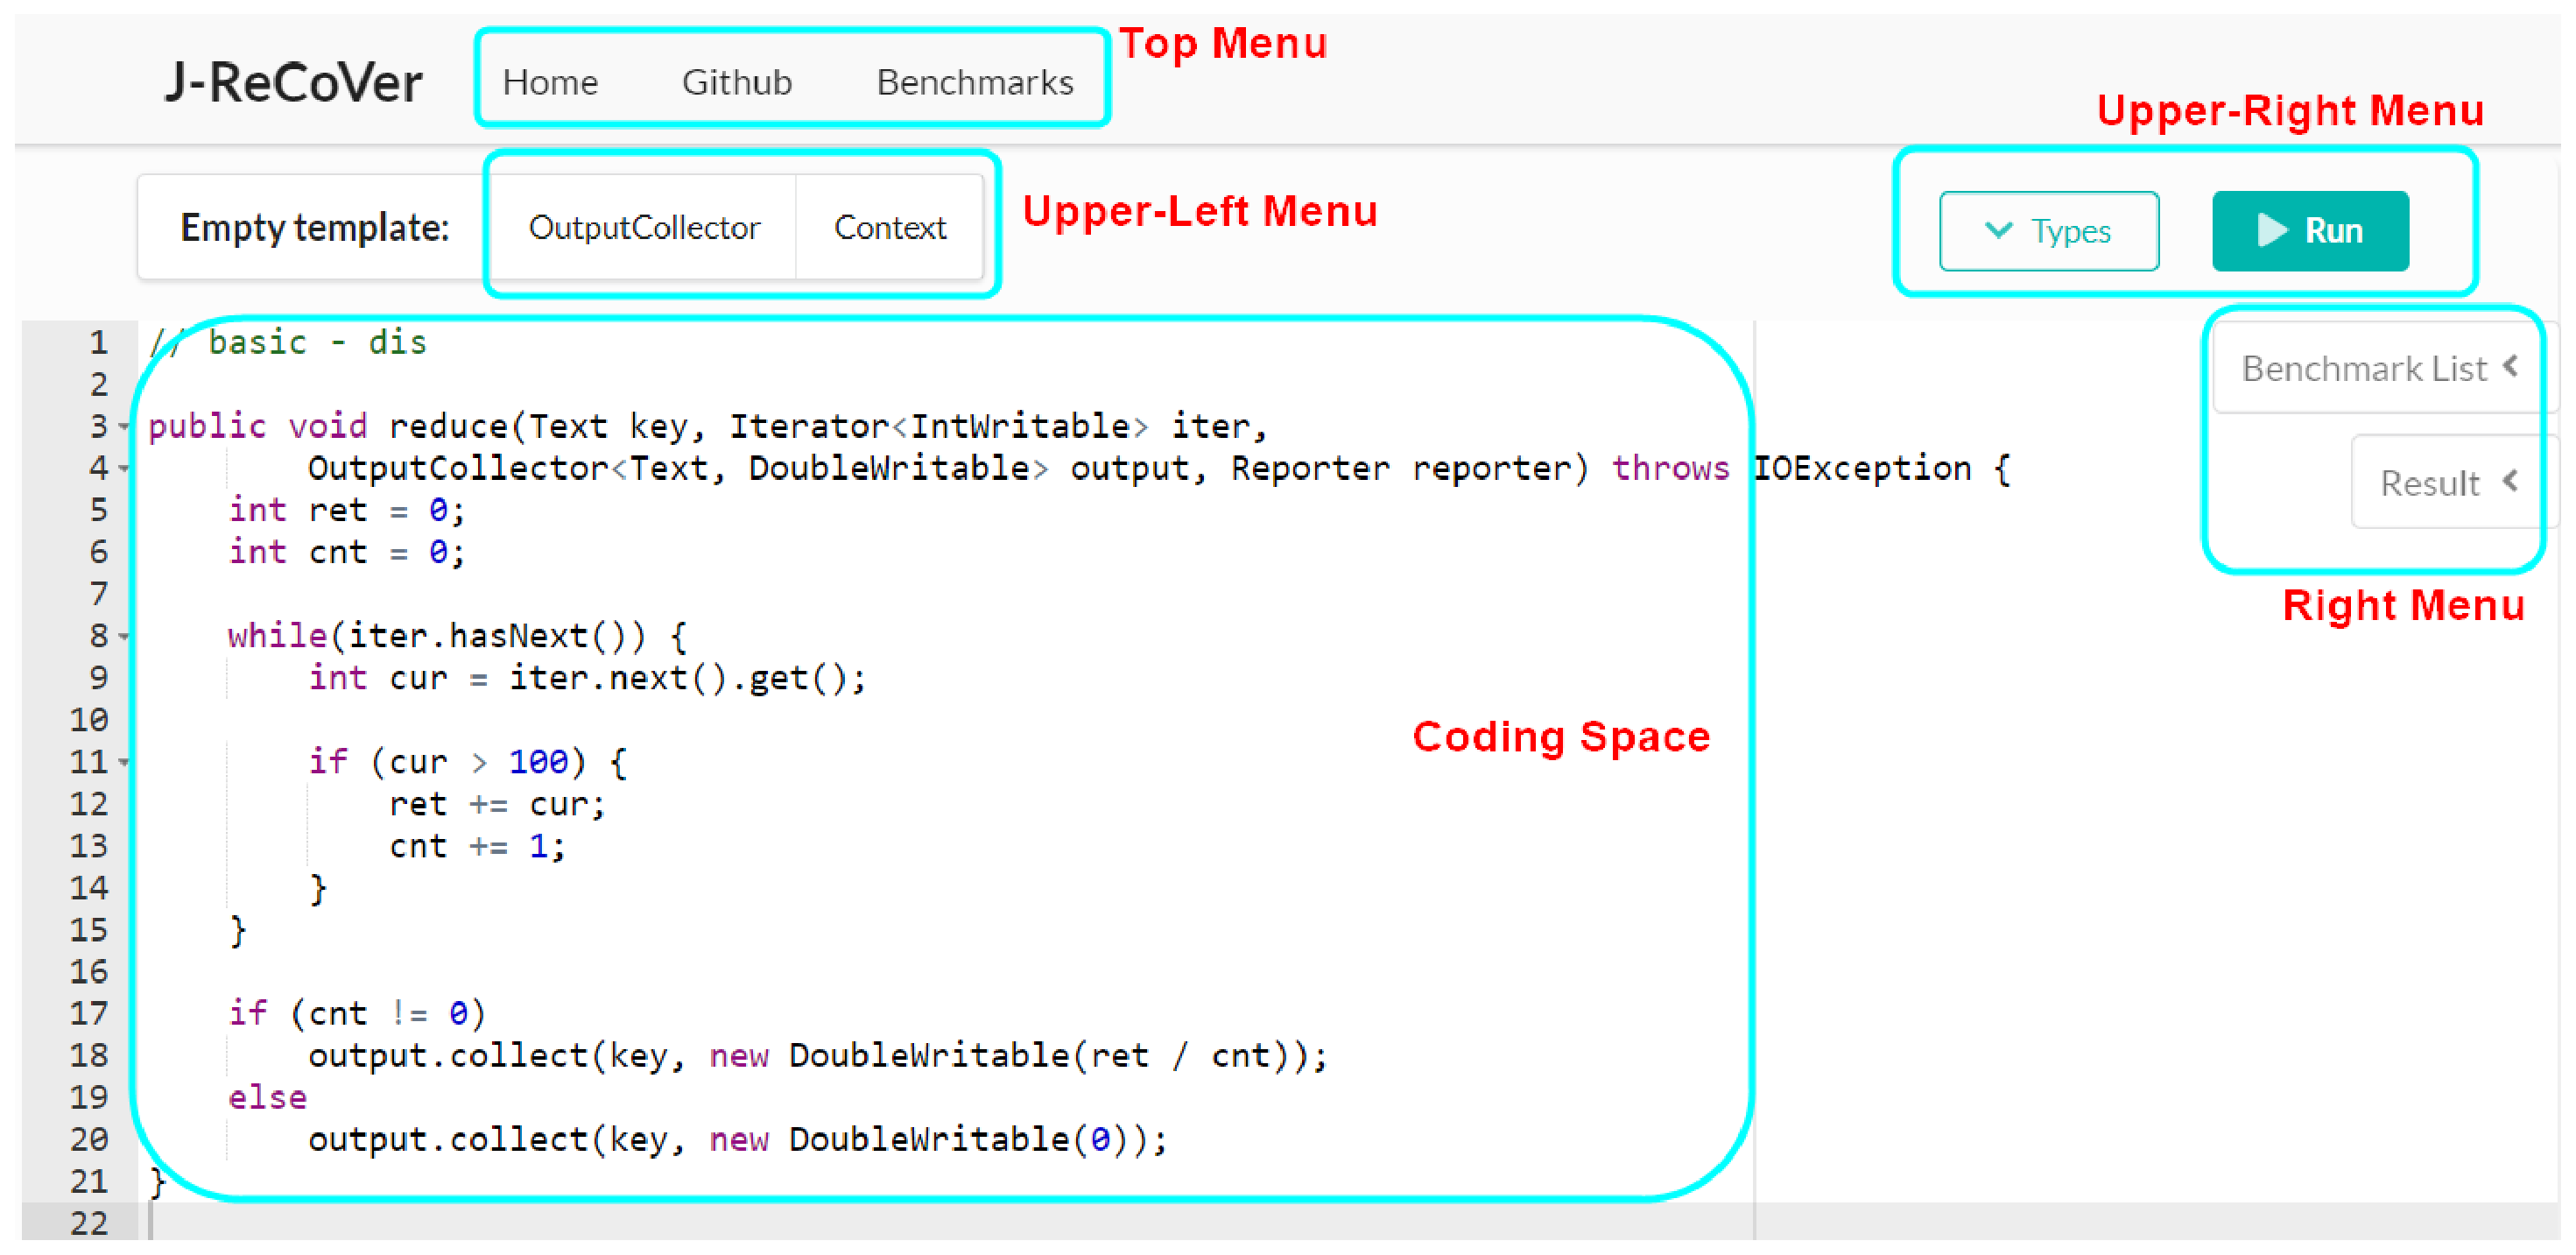
\includegraphics[width=.9\linewidth]{screenshots/main_screen_marked}
% \vspace{-5pt}
\caption{The main screen of J-ReCoVer.}
\label{fig:main_screen}
% \vspace{-15pt}
\end{center}
\end{figure}

The alignment of the user interface elements in the main screen is as follows:
\begin{itemize}
\item
Top Menu:
\begin{itemize}
\item
\emph{``GitHub''} opens a new tab of the repository of J-ReCoVer. The repository
does also contain the source code of our benchmarks.
\item
\emph{``Benchmark''} leads to the list of benchmarks we collected with their
results of commutativity analysis as Fig.~\ref{fig:benchmark_list} shows. Select
a file name or use the ``try it'' button to select an example and go back to the main screen.
\end{itemize}
\item
Right Menu:
\begin{itemize}
\item
\emph{``Benchmark List''} provides a quick selection of examples in the
benchmark (Fig.~\ref{fig:benchmark_list_right}).
\item
\emph{``Results''} shows the last analysis result.
\end{itemize}
\item
Upper-Right Menu:
\begin{itemize}
\item
\emph{``Type''} provides types that J-ReCoVer supports. Details are explained in
Appendix~\ref{appendix:3}.
\item
\emph{``Run''} starts the analysis of the selected example.
\end{itemize}
\item
Upper-Left Menu: See Appendix~\ref{appendix:3}.
\item
Coding Space.
\end{itemize}

\begin{figure}
\begin{center}
% \vspace{-10pt}
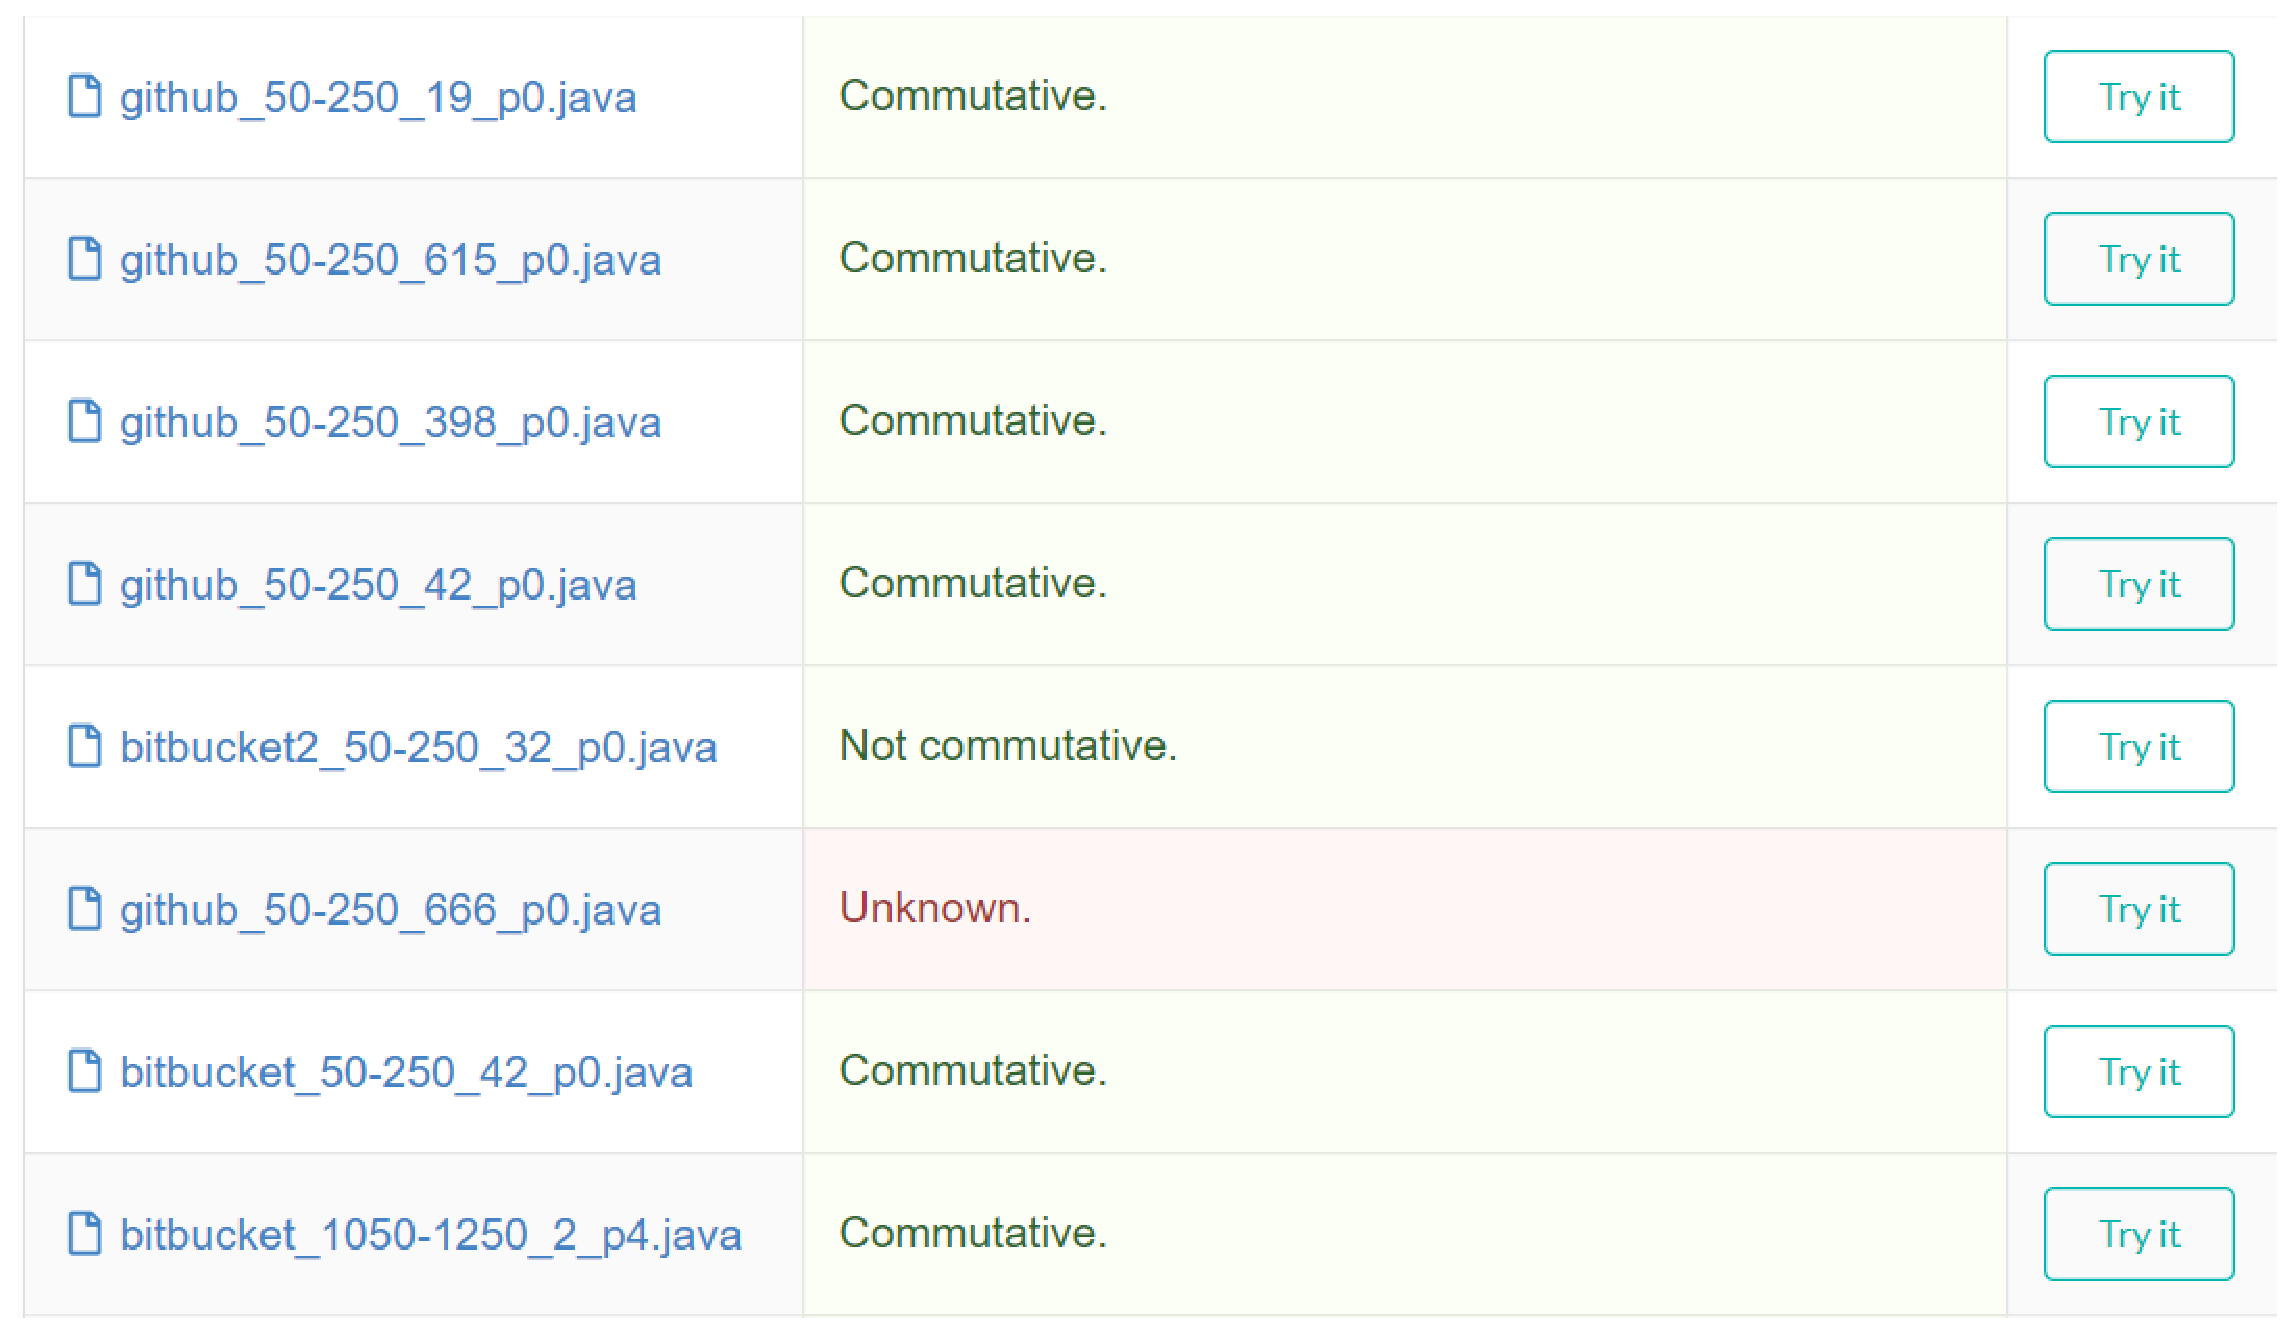
\includegraphics[width=.8\linewidth]{screenshots/benchmark_list}
% \vspace{-5pt}
\caption{A benchmark list from the top menu (a part).}
\label{fig:benchmark_list}
% \vspace{-15pt}
\end{center}
\end{figure}

\begin{figure}
\begin{center}
% \vspace{-10pt}
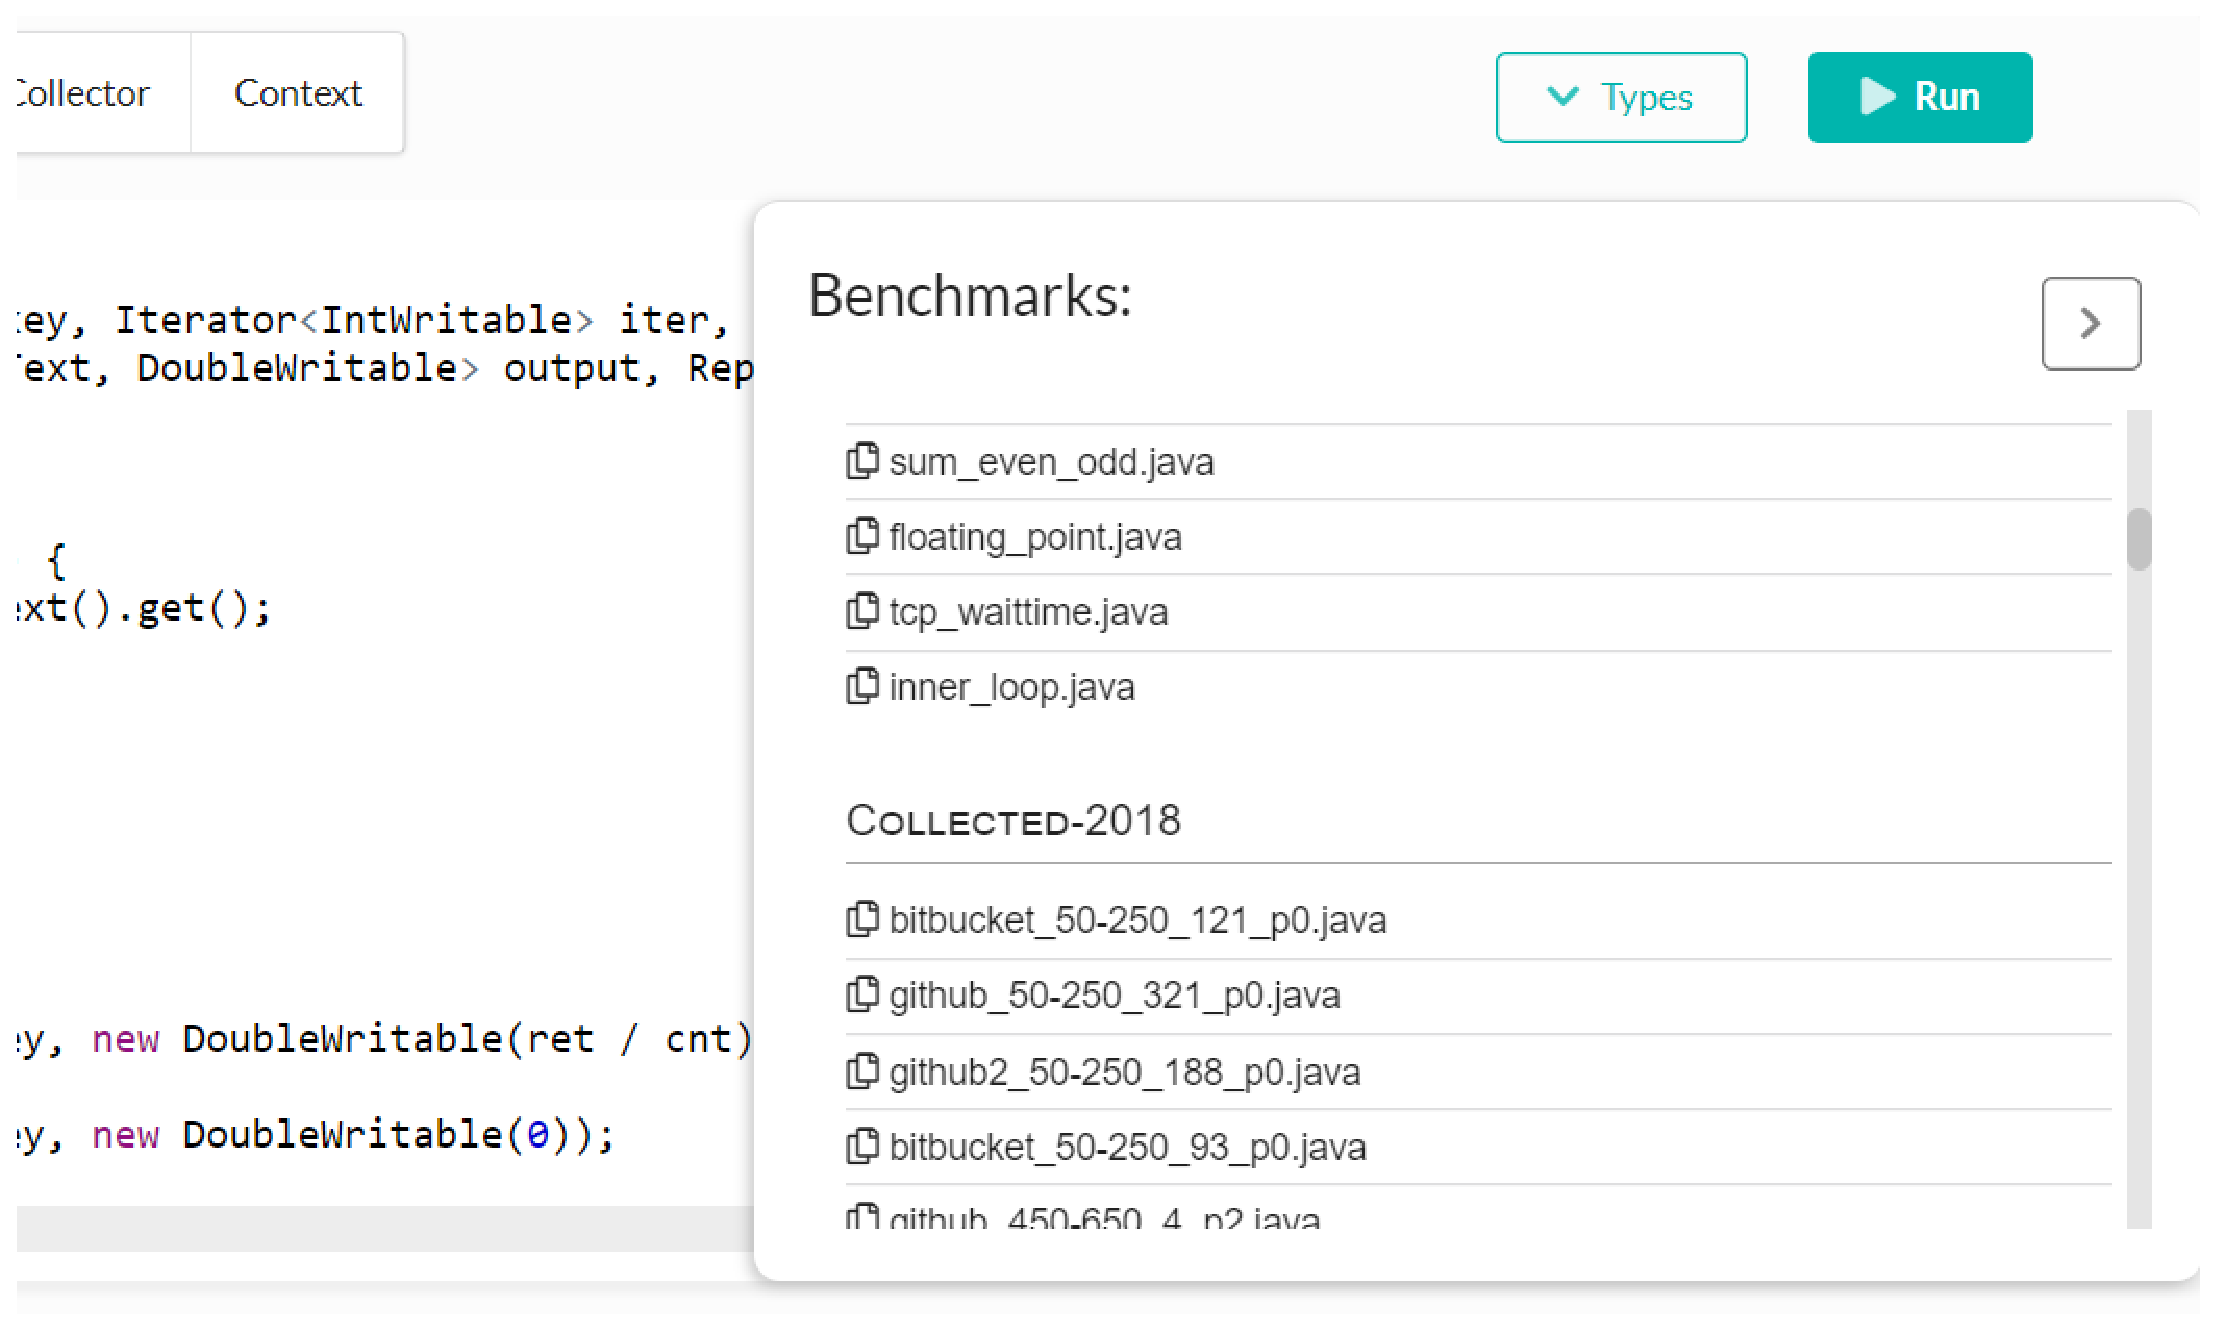
\includegraphics[width=.8\linewidth]{screenshots/benchmark_list_right}
% \vspace{-5pt}
\caption{A benchmark list from the right menu (a part).}
\label{fig:benchmark_list_right}
% \vspace{-15pt}
\end{center}
\end{figure}

\subsection{Run Analysis of a Selected Benchmark Example}
\label{appendix:2}

To run the analysis, one can choose an example from the benchmark using either
the top menu or the right menu and then click the ``Run'' button of the
upper-right menu to start the commutativity analysis of the selected example.
The pull-down menu ``Types'' of the upper-right menu provides selectable types
for input \texttt{(T1,T2)} and output \texttt{(T3,T4)} key-value pairs.
Fig.~\ref{fig:type_select_menu} shows the pull-down menu and
Fig.~\ref{fig:selectable_types} shows a part of the selectable types in
J-ReCoVer.  If one selects an example from the benchmark, the types will be
automatically selected to match the example. The selection will be needed if the
user wants to write a reduce function for analysis  from scratch (see
Appendix~\ref{appendix:3}).

\begin{figure}
\begin{center}
% \vspace{-10pt}
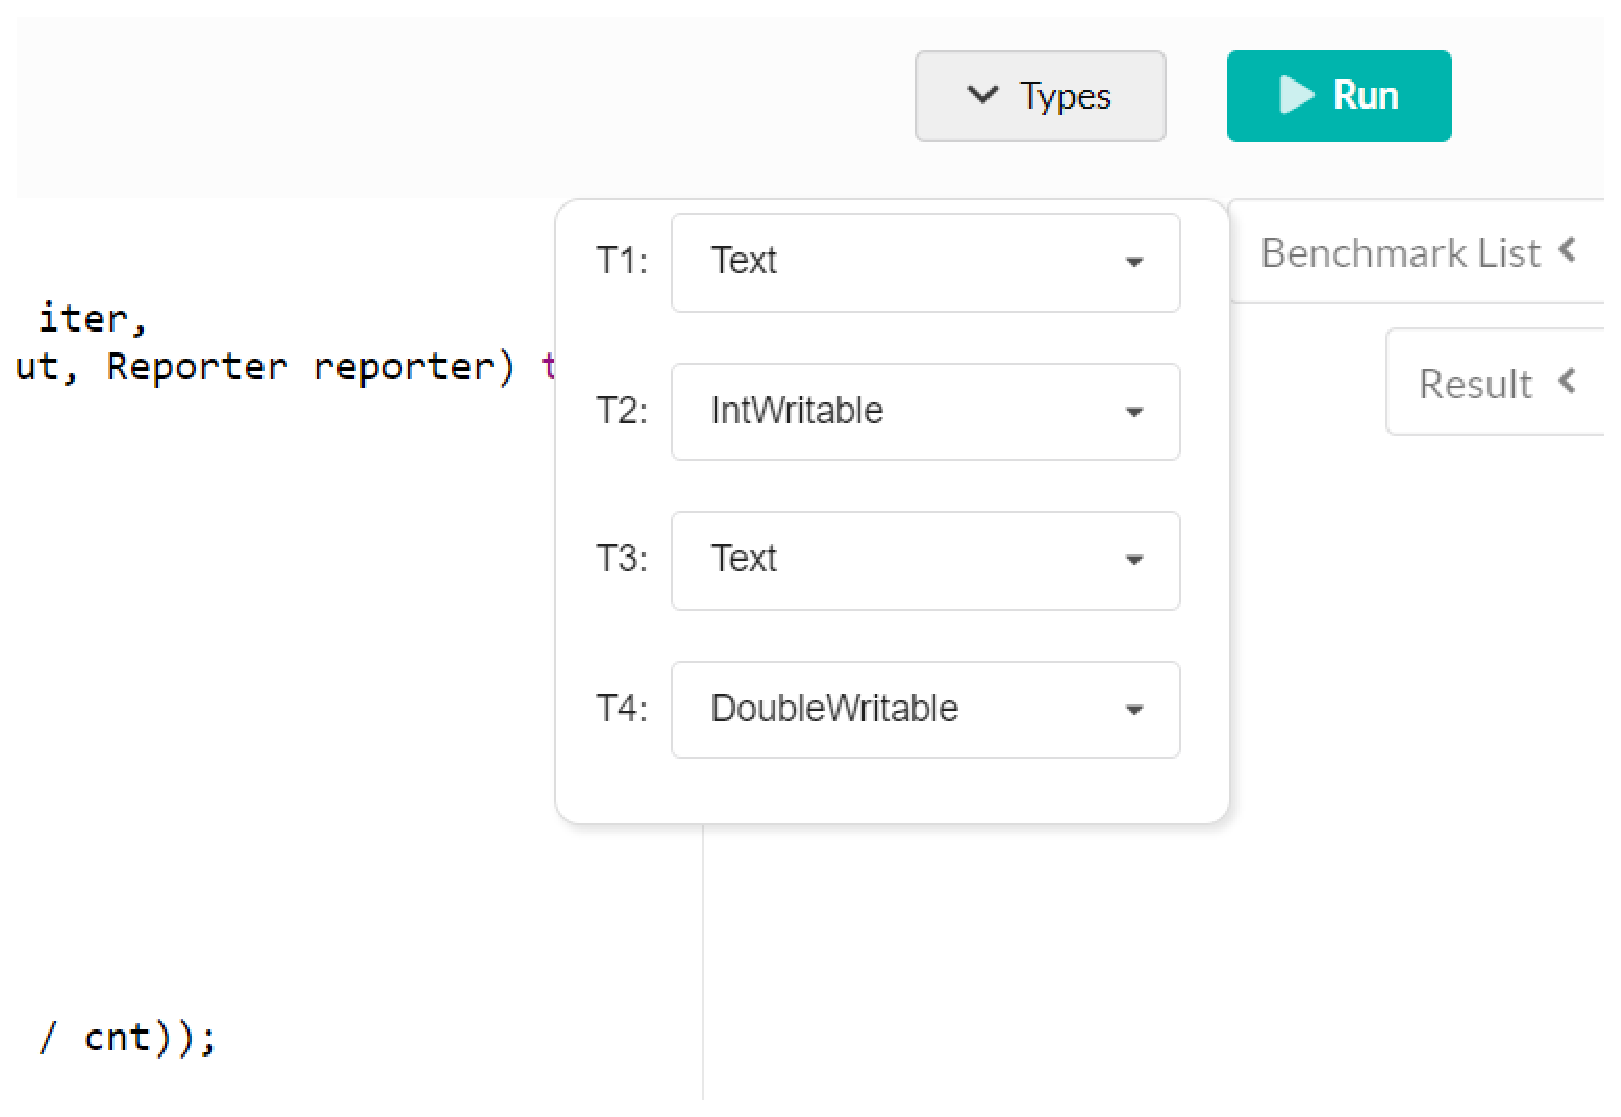
\includegraphics[width=.8\linewidth]{screenshots/type_select_menu}
% \vspace{-5pt}
\caption{The type selection menu.}
\label{fig:type_select_menu}
% \vspace{-15pt}
\end{center}
\end{figure}

\begin{figure}
\begin{center}
% \vspace{-10pt}
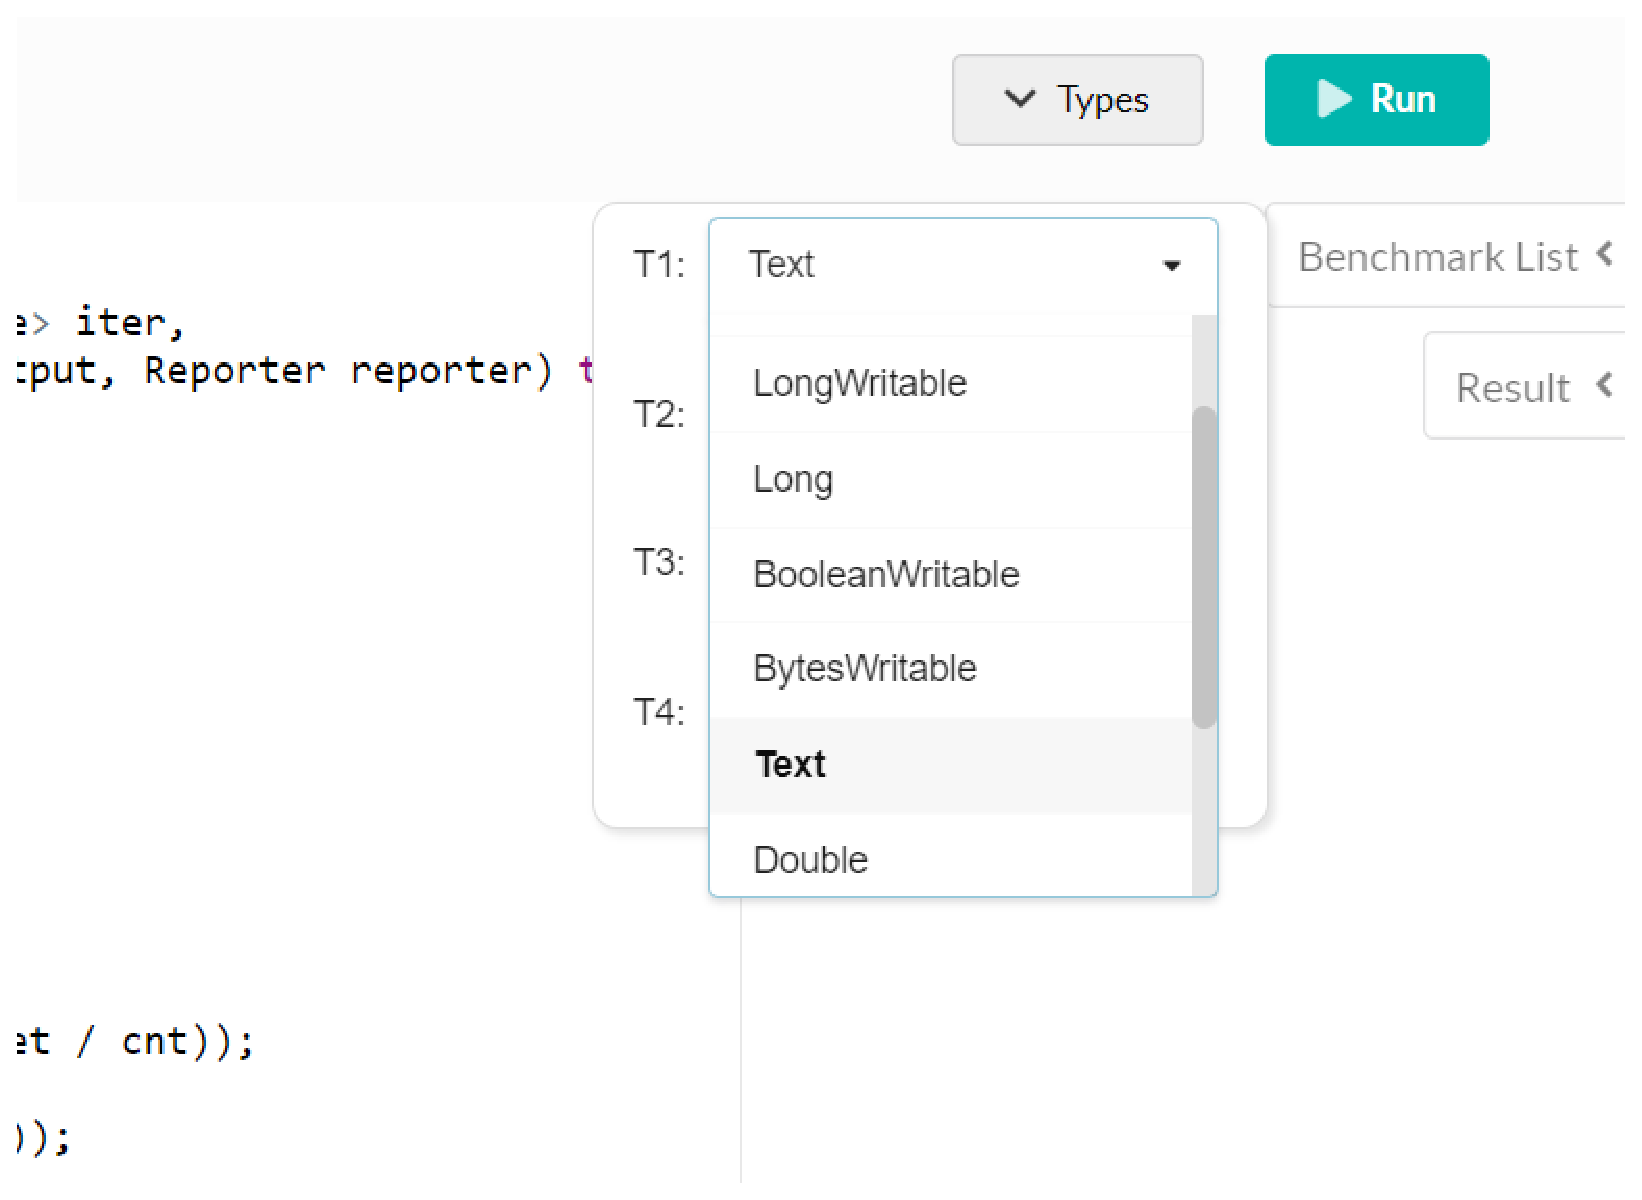
\includegraphics[width=.8\linewidth]{screenshots/selectable_types}
% \vspace{-5pt}
\caption{Selectable types (a part).}
\label{fig:selectable_types}
% \vspace{-15pt}
\end{center}
\end{figure}

After J-ReCoVer finishes the analysis, the \emph{``Result:''} tab of the right
menu will show the result of the analysis, which can be found in
Figure~\ref{fig:analysis_result}. Figure~\ref{fig:analysis_result_text} shows
the complete analysis report of the benchmark \texttt{dis.java} in
Figure~\ref{fig:main_screen}.

\begin{figure}
\begin{center}
% \vspace{-10pt}
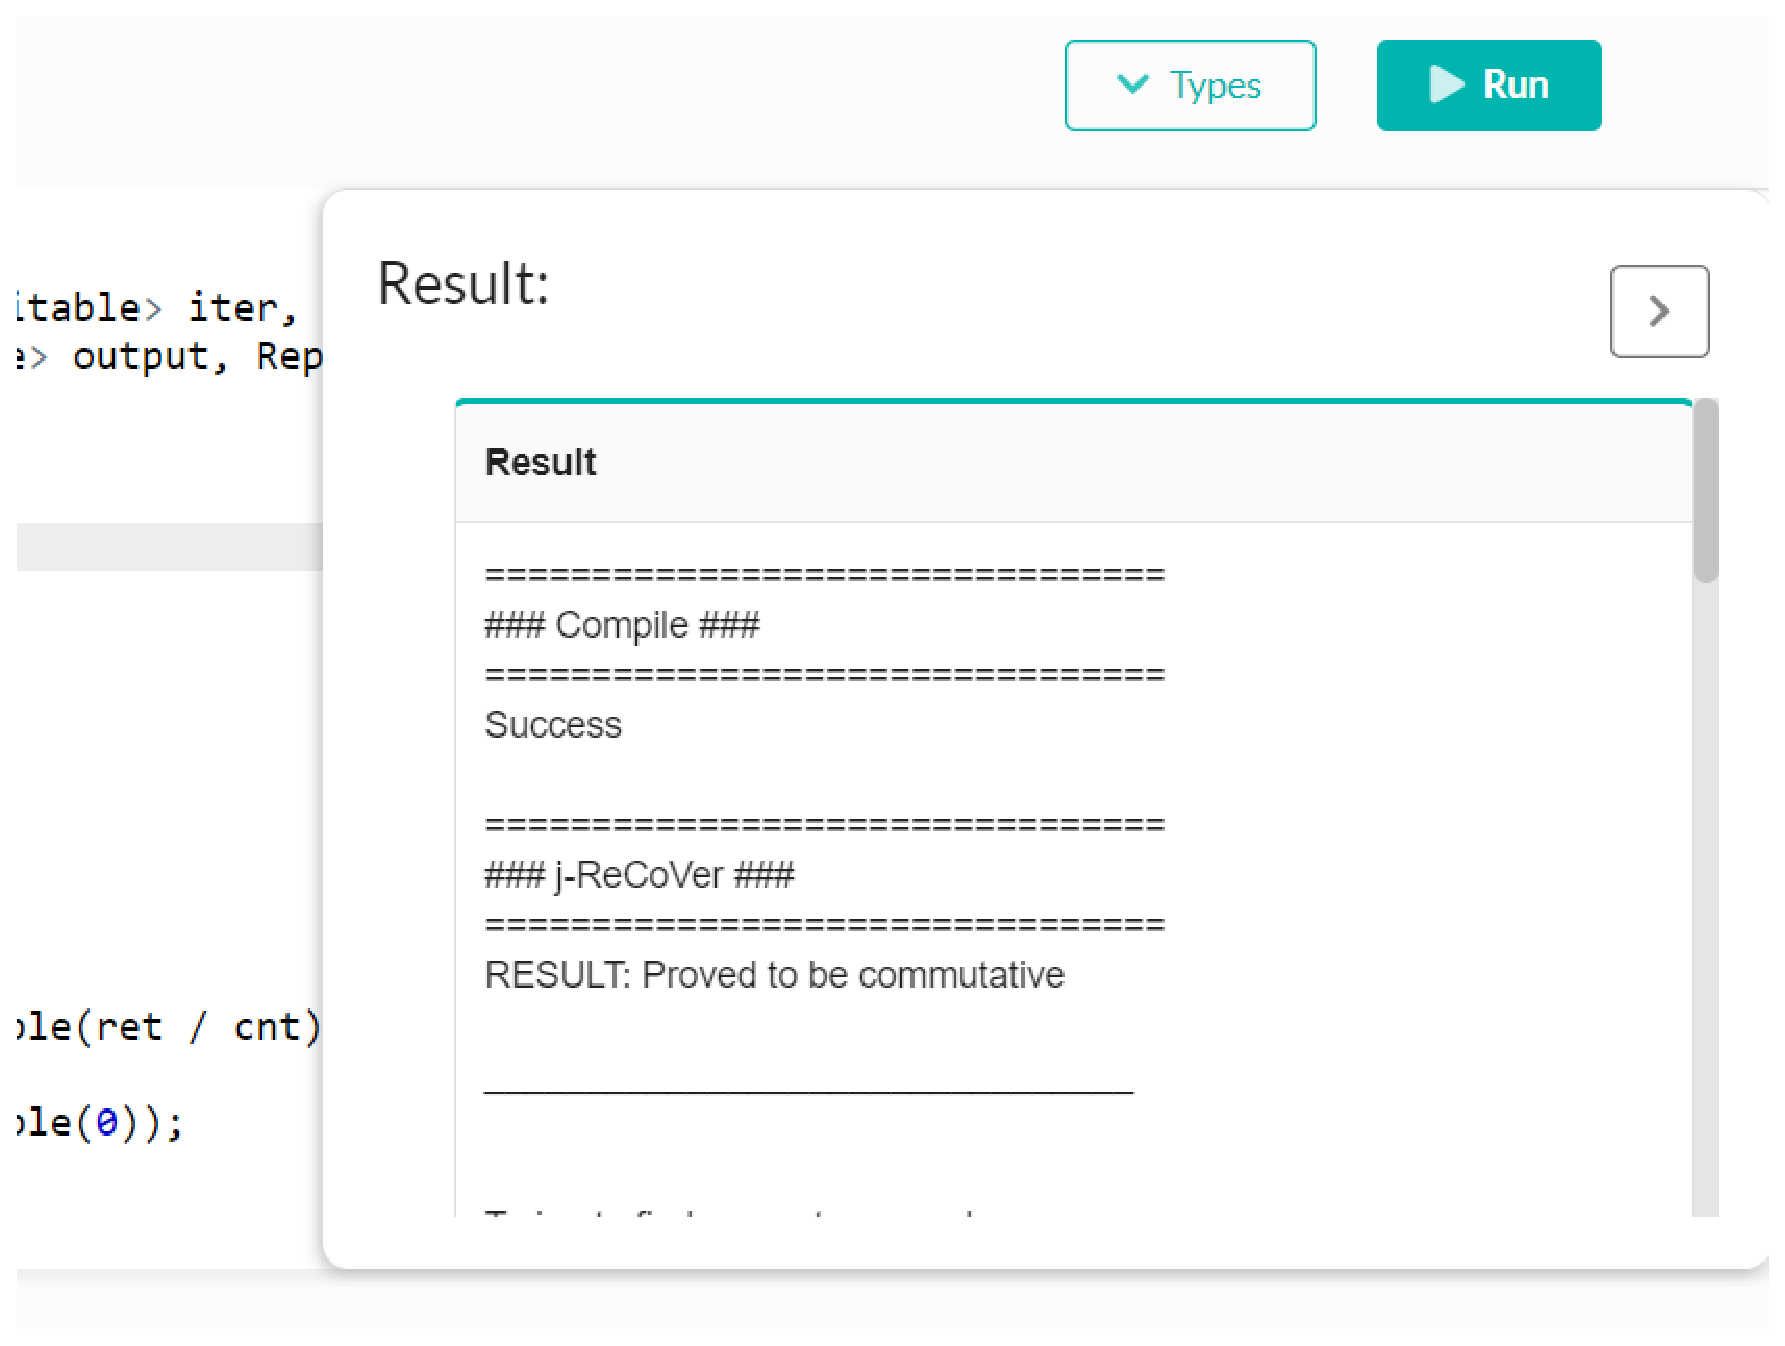
\includegraphics[width=.8\linewidth]{screenshots/analysis_result}
% \vspace{-5pt}
\caption{The analysis result.}
\label{fig:analysis_result}
% \vspace{-15pt}
\end{center}
\end{figure}

\begin{figure}
\begin{center}
\begin{mdframed}[roundcorner=5pt]
\begin{Verbatim}[fontsize=\tiny]
================================
### Compile ###
================================
Success

================================
### j-ReCoVer ###
================================
RESULT: Proved to be commutative

________________________________


Trying to find a counterexample...

RESULT: Cannot find a counterexample in 500 tests
Testcases were generated randomly.

Following are the first 50 lines of testcases:
Input1: o [5, 4, 5, 2, -1]
Input2: o [-1, 4, 5, 5, 2]
Output1: 

Key: [o]
Val: [0.0]
--
Output2: 

Key: [o]
Val: [0.0]
--------
Input1: j [1, -1, 0, 3, -2]
Input2: j [0, 3, -2, 1, -1]
Output1: 

Key: [j]
Val: [0.0]
--
Output2: 

Key: [j]
Val: [0.0]
--------
Input1: e [4, 3, 5, -4, 1]
Input2: e [4, -4, 5, 3, 1]
Output1: 

Key: [e]
Val: [0.0]
--
Output2: 

Key: [e]
Val: [0.0]
--------
Input1: s [3, 0, 2, -4, -1]
Input2: s [3, -1, 0, -4, 2]
Output1: 

Key: [s]
Val: [0.0]
--
Output2: 

Key: [s]
Val: [0.0]
--------
Input1: v [-3, -2, 3, 3, -3]
Input2: v [3, -2, -3, -3, 3]
\end{Verbatim}
\end{mdframed}
\caption{The analysis result of \texttt{dis.java}.}
\label{fig:analysis_result_text}
\end{center}
\end{figure}

When an analysis is started, J-ReCoVer first tries to compile the chosen example
and then performs its commutativity analysis. If the analysis cannot conclude
that the example is commutative, J-ReCoVer then runs 500 randomly generated test
cases to try to find a counterexample. If the test cases all pass, then the
result will be ``unknown''.

\clearpage
\subsection{Run Analysis of a User-defined Reducer Function}
\label{appendix:3}

Besides examples from the benchmark, J-ReCoVer also provides an interactive way
for analysing a user-defined reducer function.  One can directly edit the code
of a selected example in the coding space for further analysis, or write a
reducer function from scratch. The upper-left menu (below the top menu)
provides blank templates for two versions of Hadoop. The templates are shown
below:

\begin{mdframed}[roundcorner=5pt]
\begin{verbatim}
public void reduce(T1 key, Iterator<T2> values,
	OutputCollector<T3,T4> oc1, Reporter reporter)
		throws IOException,InterruptedException {

}
\end{verbatim}
\end{mdframed}

\begin{mdframed}[roundcorner=5pt]
\begin{verbatim}
public void reduce(T1 key, Iterable<T2> values,
	Context context) throws IOException,InterruptedException {

}
\end{verbatim}
\end{mdframed}

In this case, one would have to manually fill the types T1 to T4 and the
function body, and then select the types from the pull-down menu as shown in
Figure~\ref{fig:type_select_menu} and Figure~\ref{fig:selectable_types}. All
selectable types are:

\begin{itemize}
\item Long,
\item BooleanWritable,
\item BytesWritable,
\item Text,
\item Double,
\item DoubleWritable,
\item Float,
\item FloatWritable.
\end{itemize}

\clearpage
\appendix

\section{J-ReCoVer Demo}

Our plan is to demonstrate the basic usage of J-ReCoVer on two examples. The
first example is a reducer that is not commutative, and J-ReCoVer will report a
counterexample. Based on this counterexample, we will fix the reducer to get the
second example, and let J-ReCoVer to check it again. Now, J-ReCoVer will report
that the reducer is commutative. Below, we give a more detailed description of
the functionalities of J-ReCoVer. 

\subsection{The User Interface of J-ReCoVer}
\label{appendix:1}

Figure~\ref{fig:main_screen} shows the main screen of J-ReCoVer. 

\begin{figure}
\begin{center}
% \vspace{-10pt}
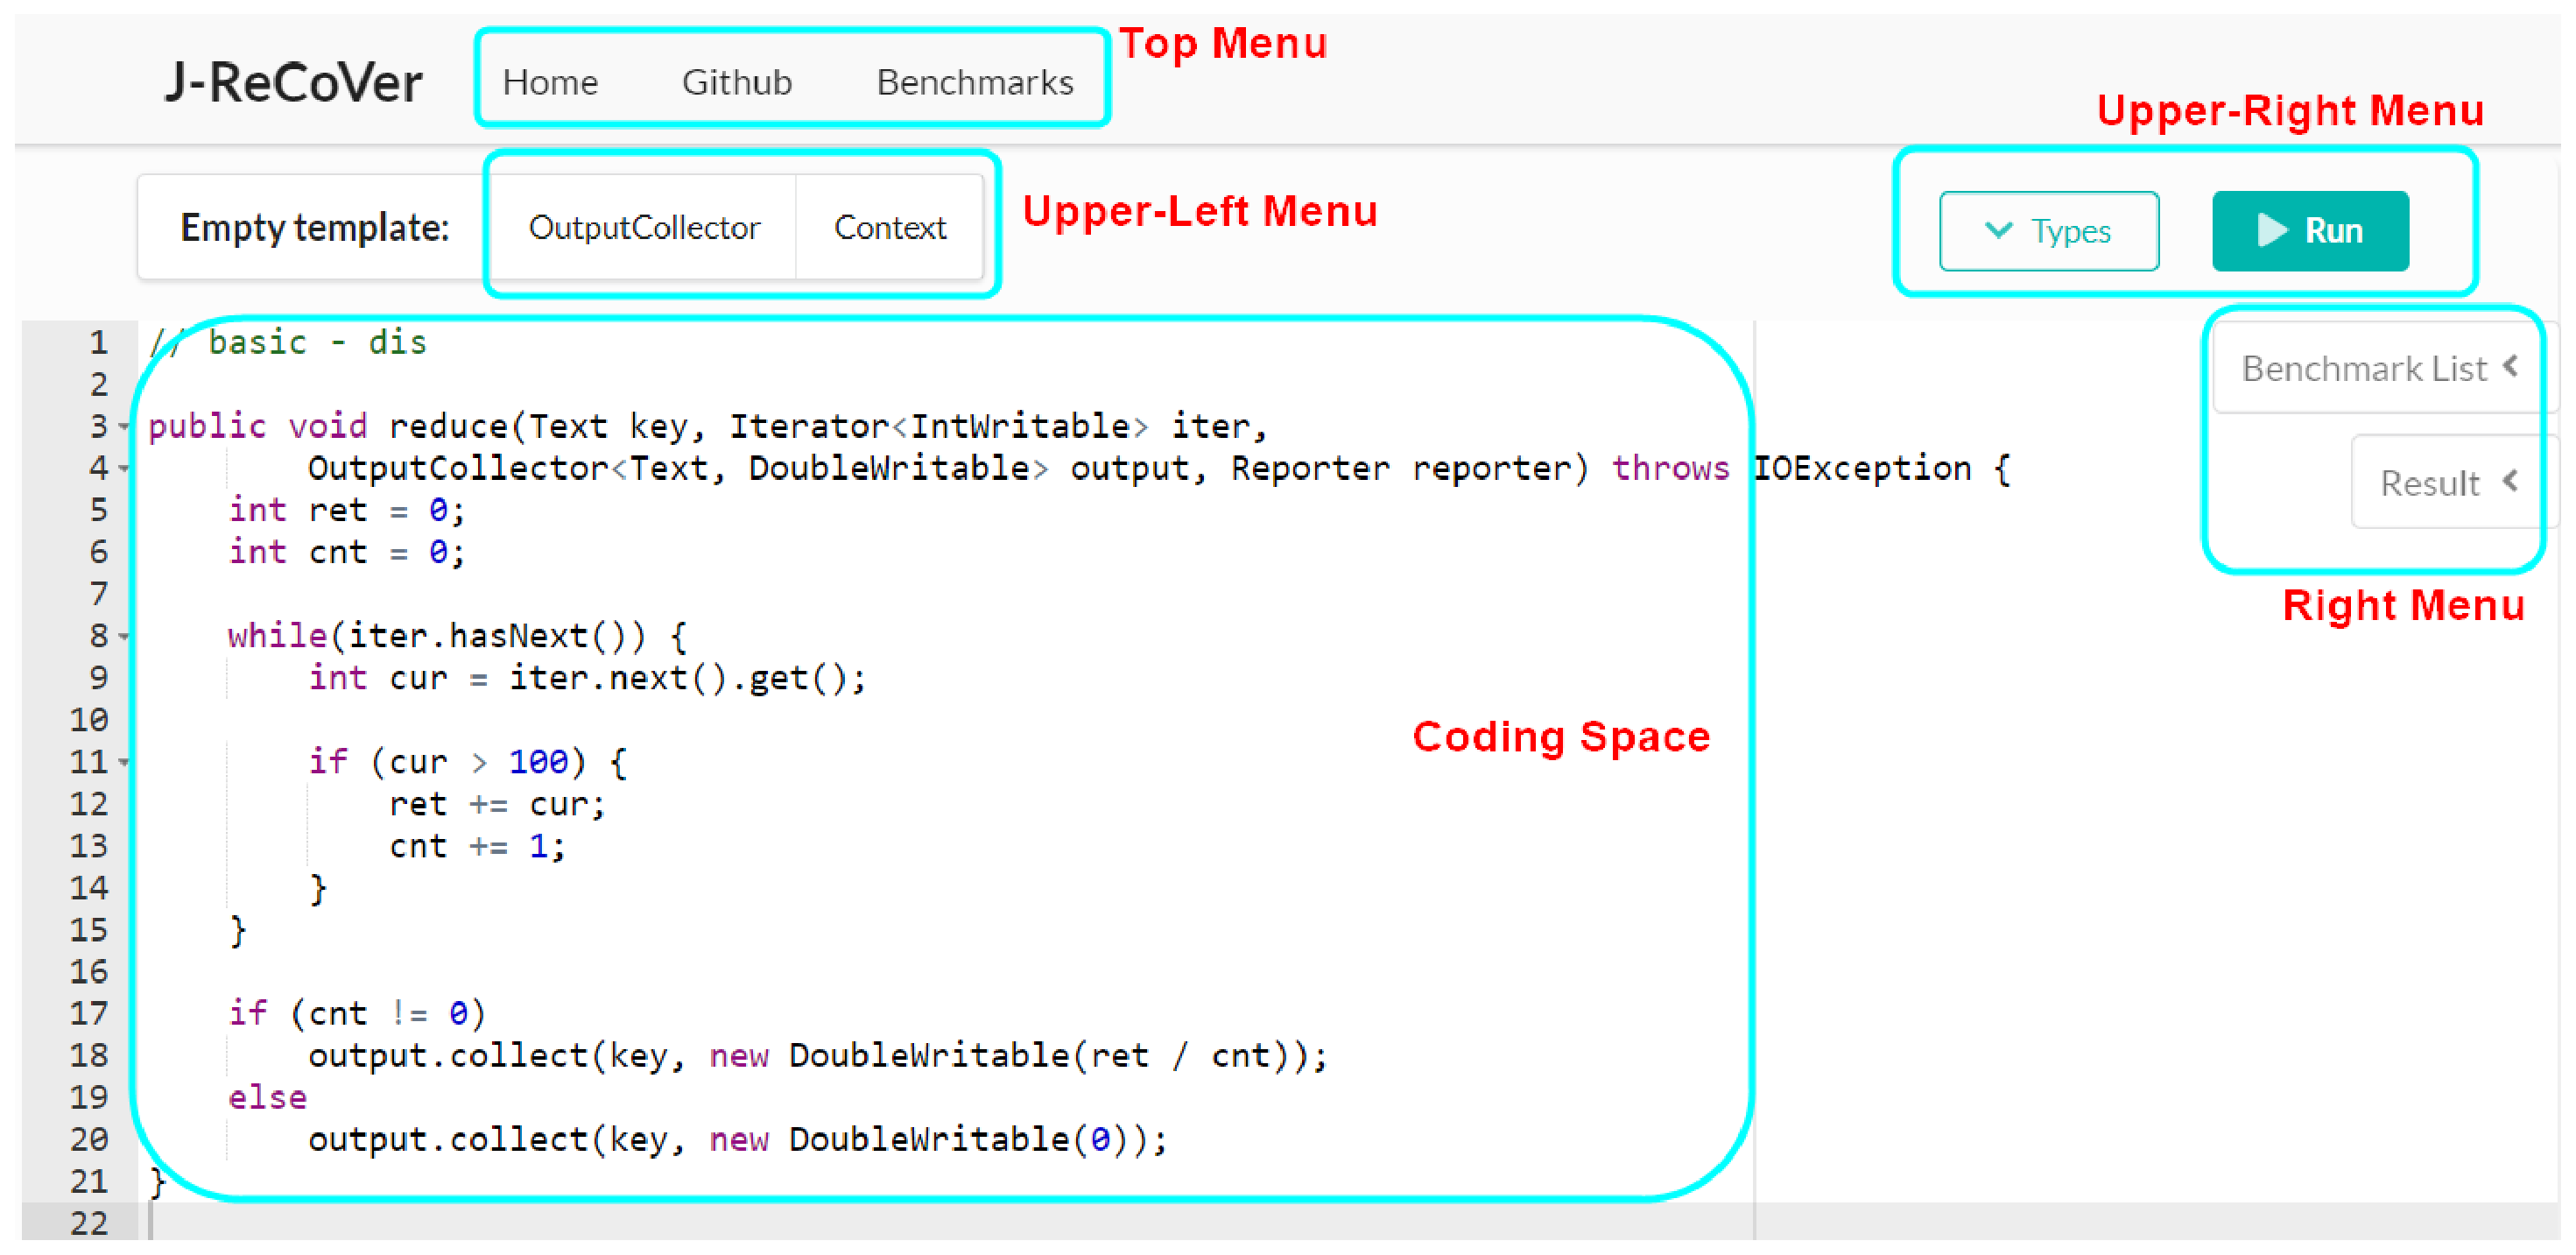
\includegraphics[width=.9\linewidth]{screenshots/main_screen_marked}
% \vspace{-5pt}
\caption{The main screen of J-ReCoVer.}
\label{fig:main_screen}
% \vspace{-15pt}
\end{center}
\end{figure}

The alignment of the user interface elements in the main screen is as follows:
\begin{itemize}
\item
Top Menu:
\begin{itemize}
\item
\emph{``GitHub''} opens a new tab of the repository of J-ReCoVer. The repository
does also contain the source code of our benchmarks.
\item
\emph{``Benchmark''} leads to the list of benchmarks we collected with their
results of commutativity analysis as Fig.~\ref{fig:benchmark_list} shows. Select
a file name or use the ``try it'' button to select an example and go back to the main screen.
\end{itemize}
\item
Right Menu:
\begin{itemize}
\item
\emph{``Benchmark List''} provides a quick selection of examples in the
benchmark (Fig.~\ref{fig:benchmark_list_right}).
\item
\emph{``Results''} shows the last analysis result.
\end{itemize}
\item
Upper-Right Menu:
\begin{itemize}
\item
\emph{``Type''} provides types that J-ReCoVer supports. Details are explained in
Appendix~\ref{appendix:3}.
\item
\emph{``Run''} starts the analysis of the selected example.
\end{itemize}
\item
Upper-Left Menu: See Appendix~\ref{appendix:3}.
\item
Coding Space.
\end{itemize}

\begin{figure}
\begin{center}
% \vspace{-10pt}
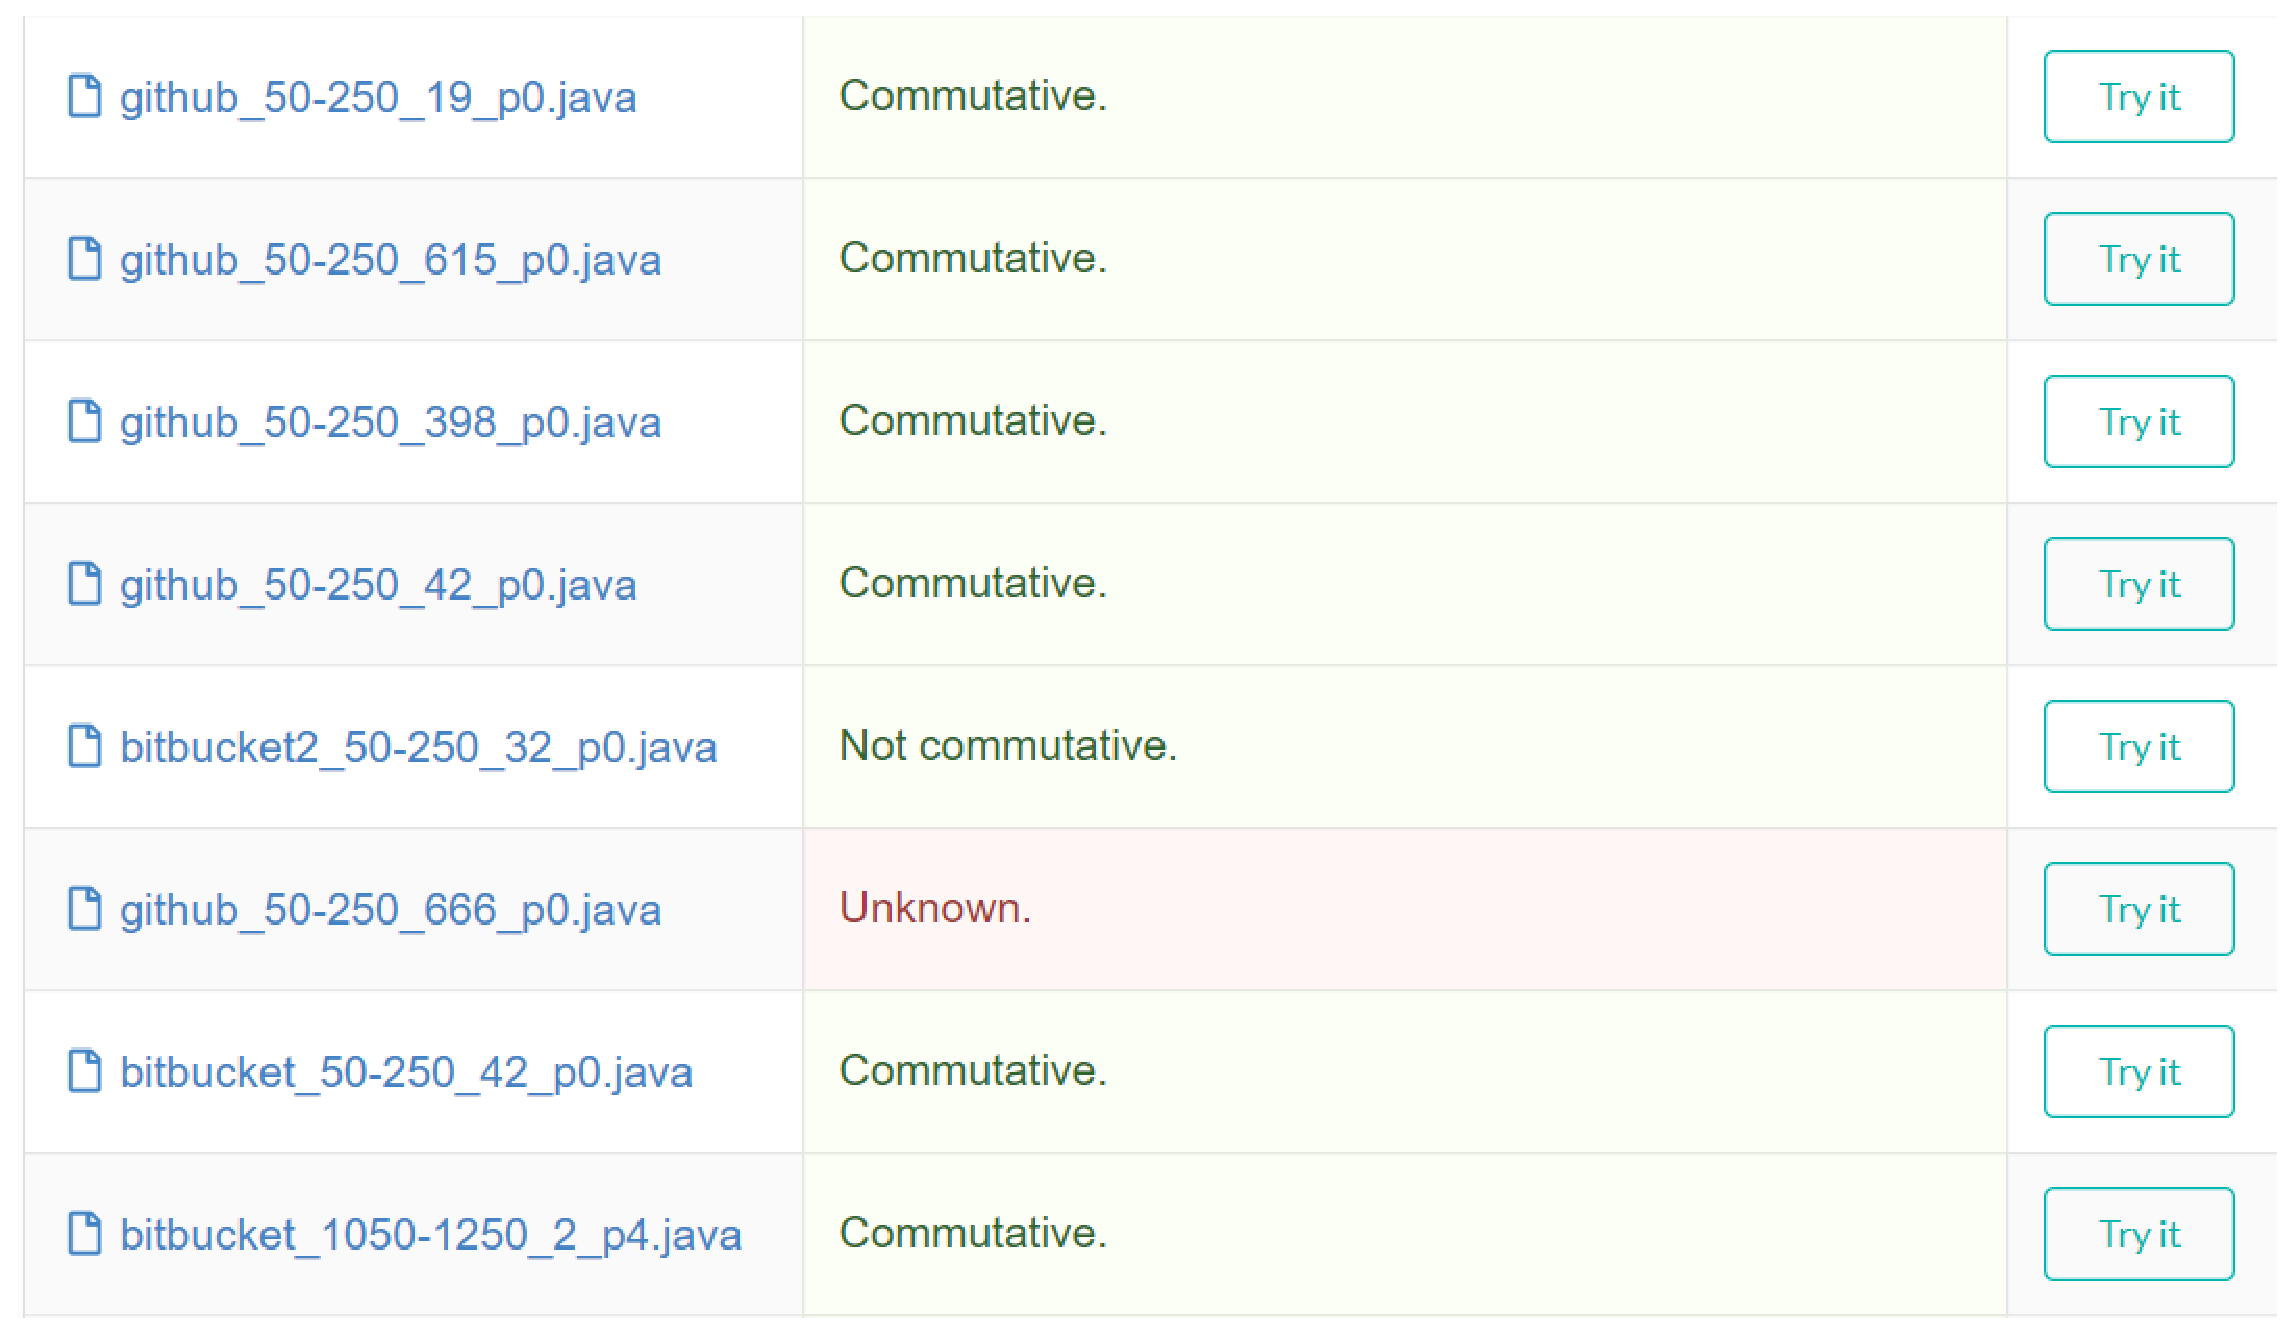
\includegraphics[width=.8\linewidth]{screenshots/benchmark_list}
% \vspace{-5pt}
\caption{A benchmark list from the top menu (a part).}
\label{fig:benchmark_list}
% \vspace{-15pt}
\end{center}
\end{figure}

\begin{figure}
\begin{center}
% \vspace{-10pt}
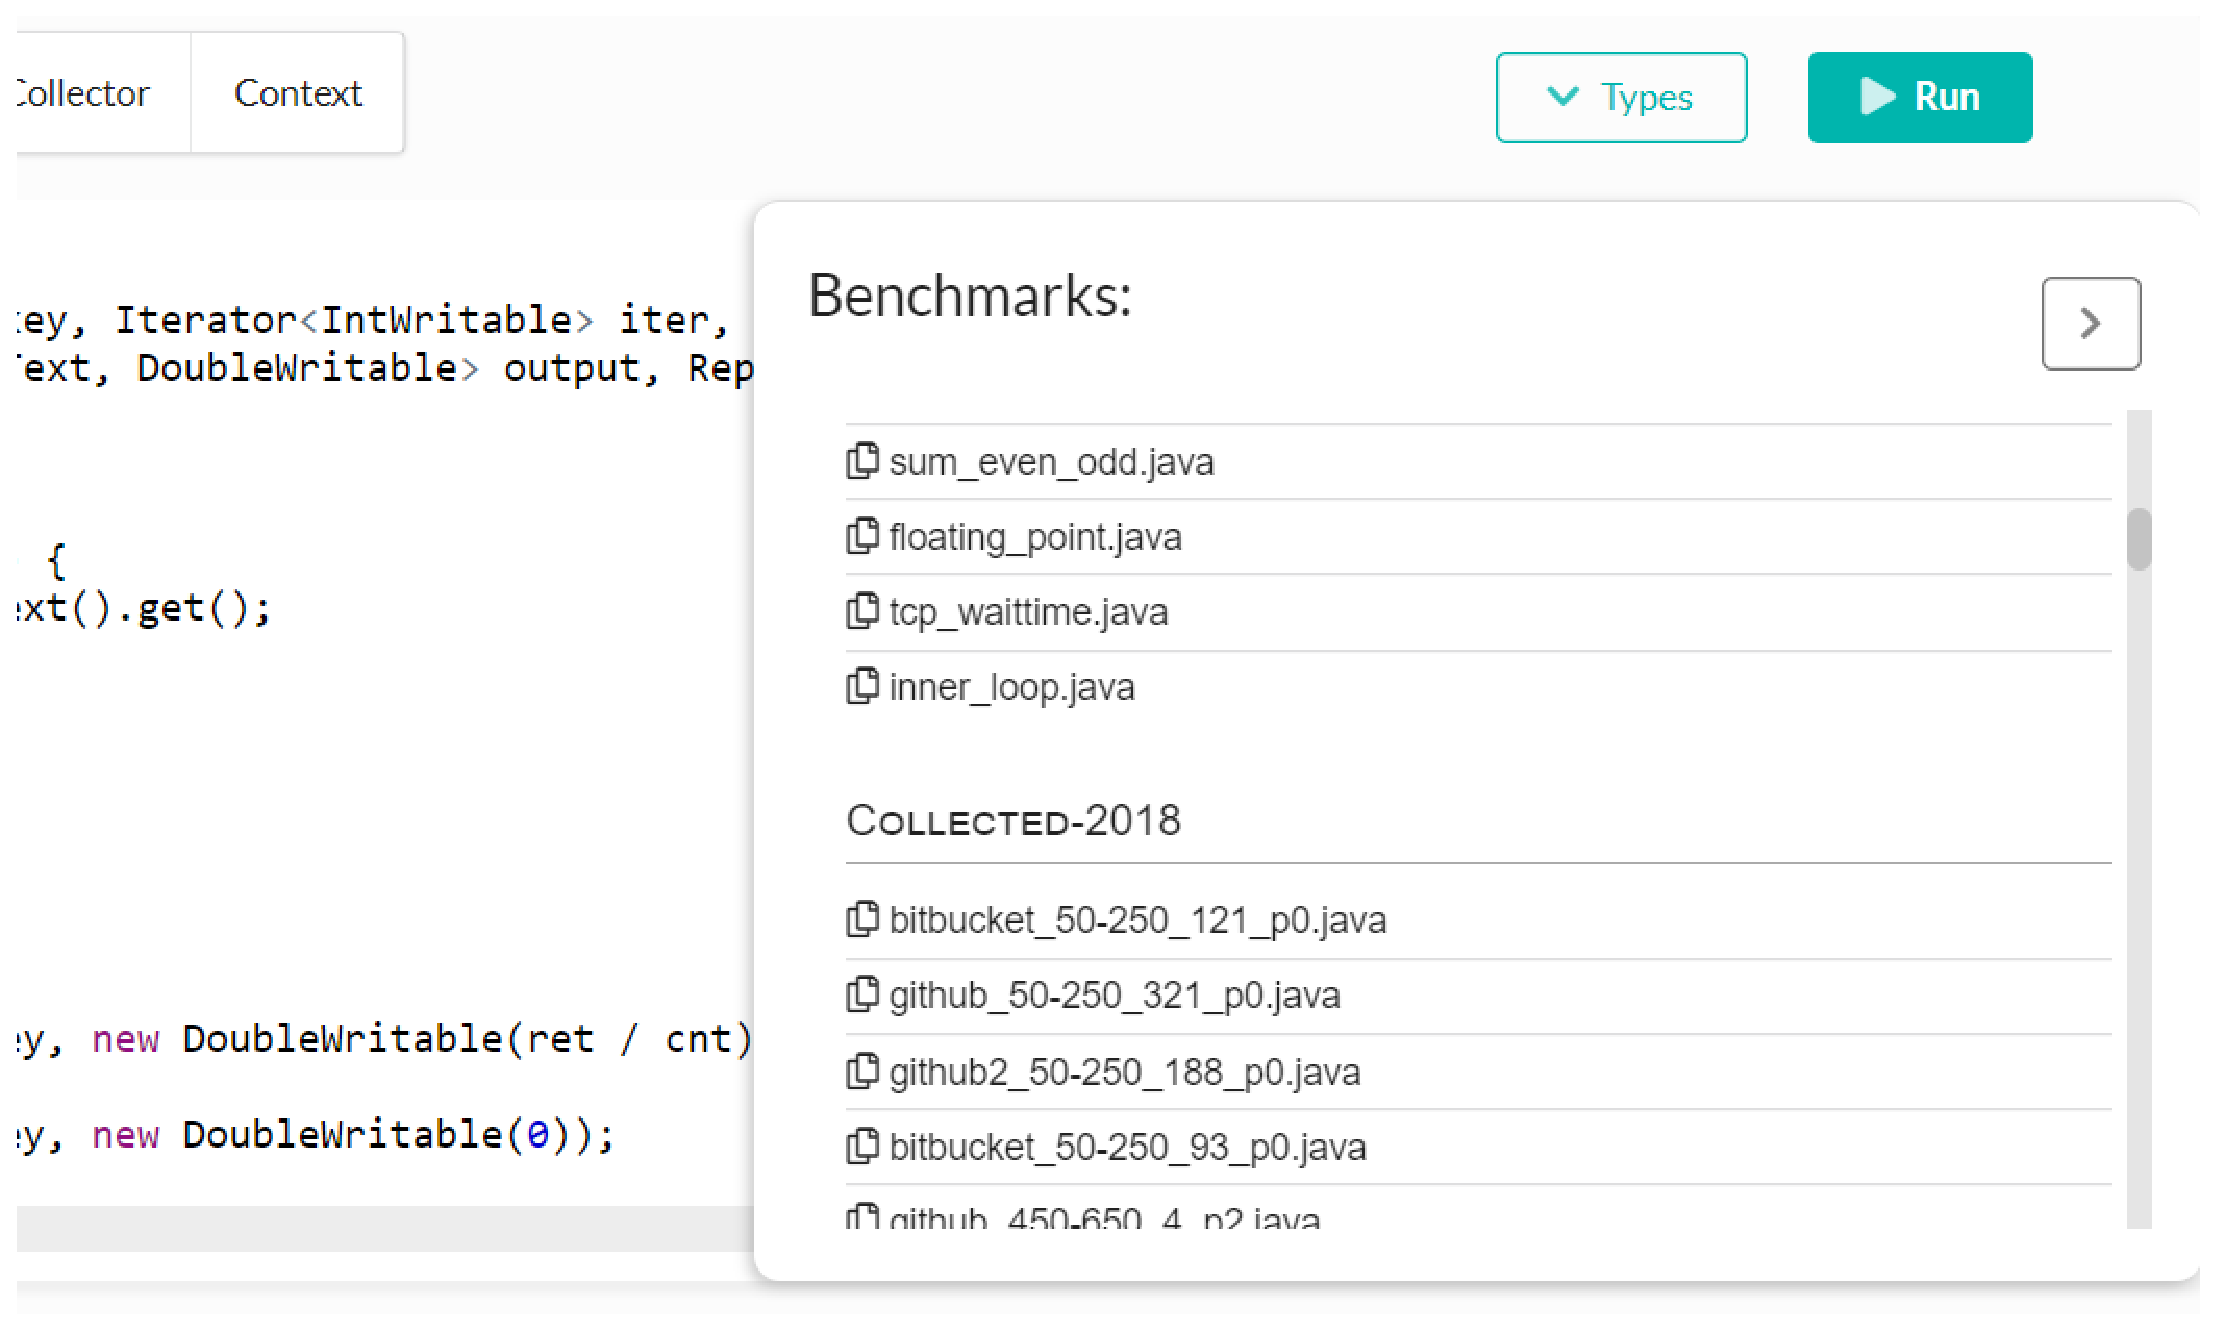
\includegraphics[width=.8\linewidth]{screenshots/benchmark_list_right}
% \vspace{-5pt}
\caption{A benchmark list from the right menu (a part).}
\label{fig:benchmark_list_right}
% \vspace{-15pt}
\end{center}
\end{figure}

\subsection{Run Analysis of a Selected Benchmark Example}
\label{appendix:2}

To run the analysis, one can choose an example from the benchmark using either
the top menu or the right menu and then click the ``Run'' button of the
upper-right menu to start the commutativity analysis of the selected example.
The pull-down menu ``Types'' of the upper-right menu provides selectable types
for input \texttt{(T1,T2)} and output \texttt{(T3,T4)} key-value pairs.
Fig.~\ref{fig:type_select_menu} shows the pull-down menu and
Fig.~\ref{fig:selectable_types} shows a part of the selectable types in
J-ReCoVer.  If one selects an example from the benchmark, the types will be
automatically selected to match the example. The selection will be needed if the
user wants to write a reduce function for analysis  from scratch (see
Appendix~\ref{appendix:3}).

\begin{figure}
\begin{center}
% \vspace{-10pt}
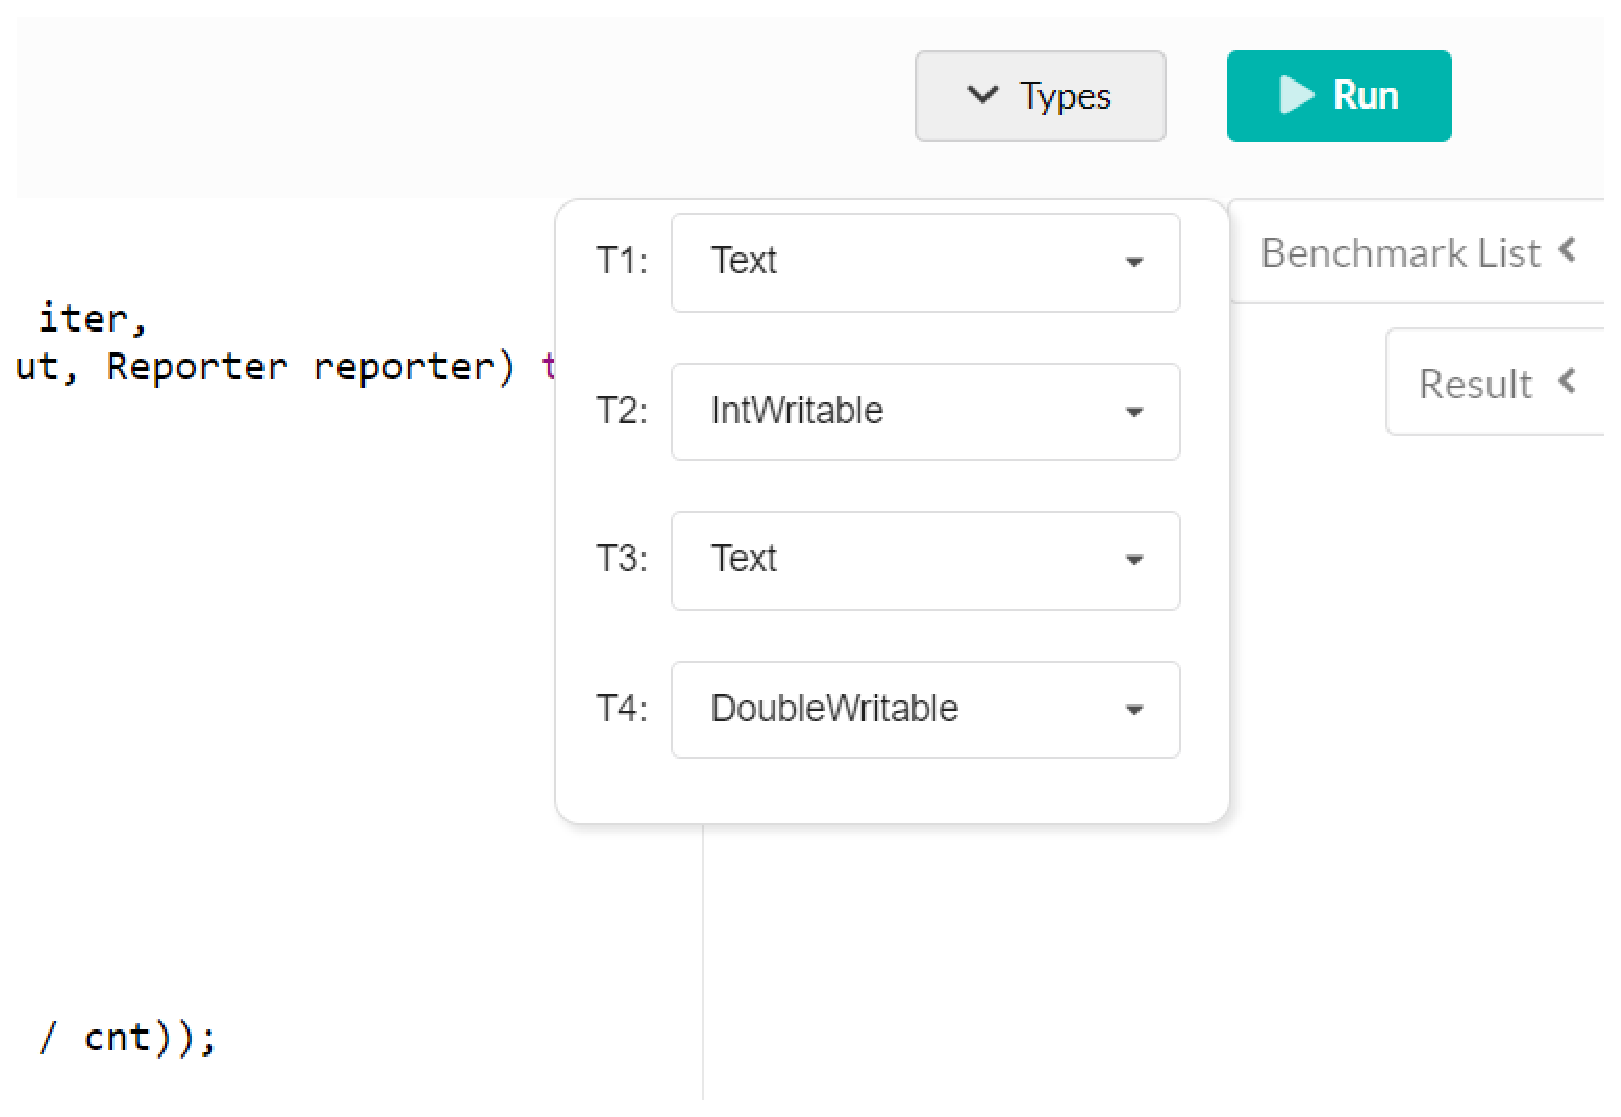
\includegraphics[width=.8\linewidth]{screenshots/type_select_menu}
% \vspace{-5pt}
\caption{The type selection menu.}
\label{fig:type_select_menu}
% \vspace{-15pt}
\end{center}
\end{figure}

\begin{figure}
\begin{center}
% \vspace{-10pt}
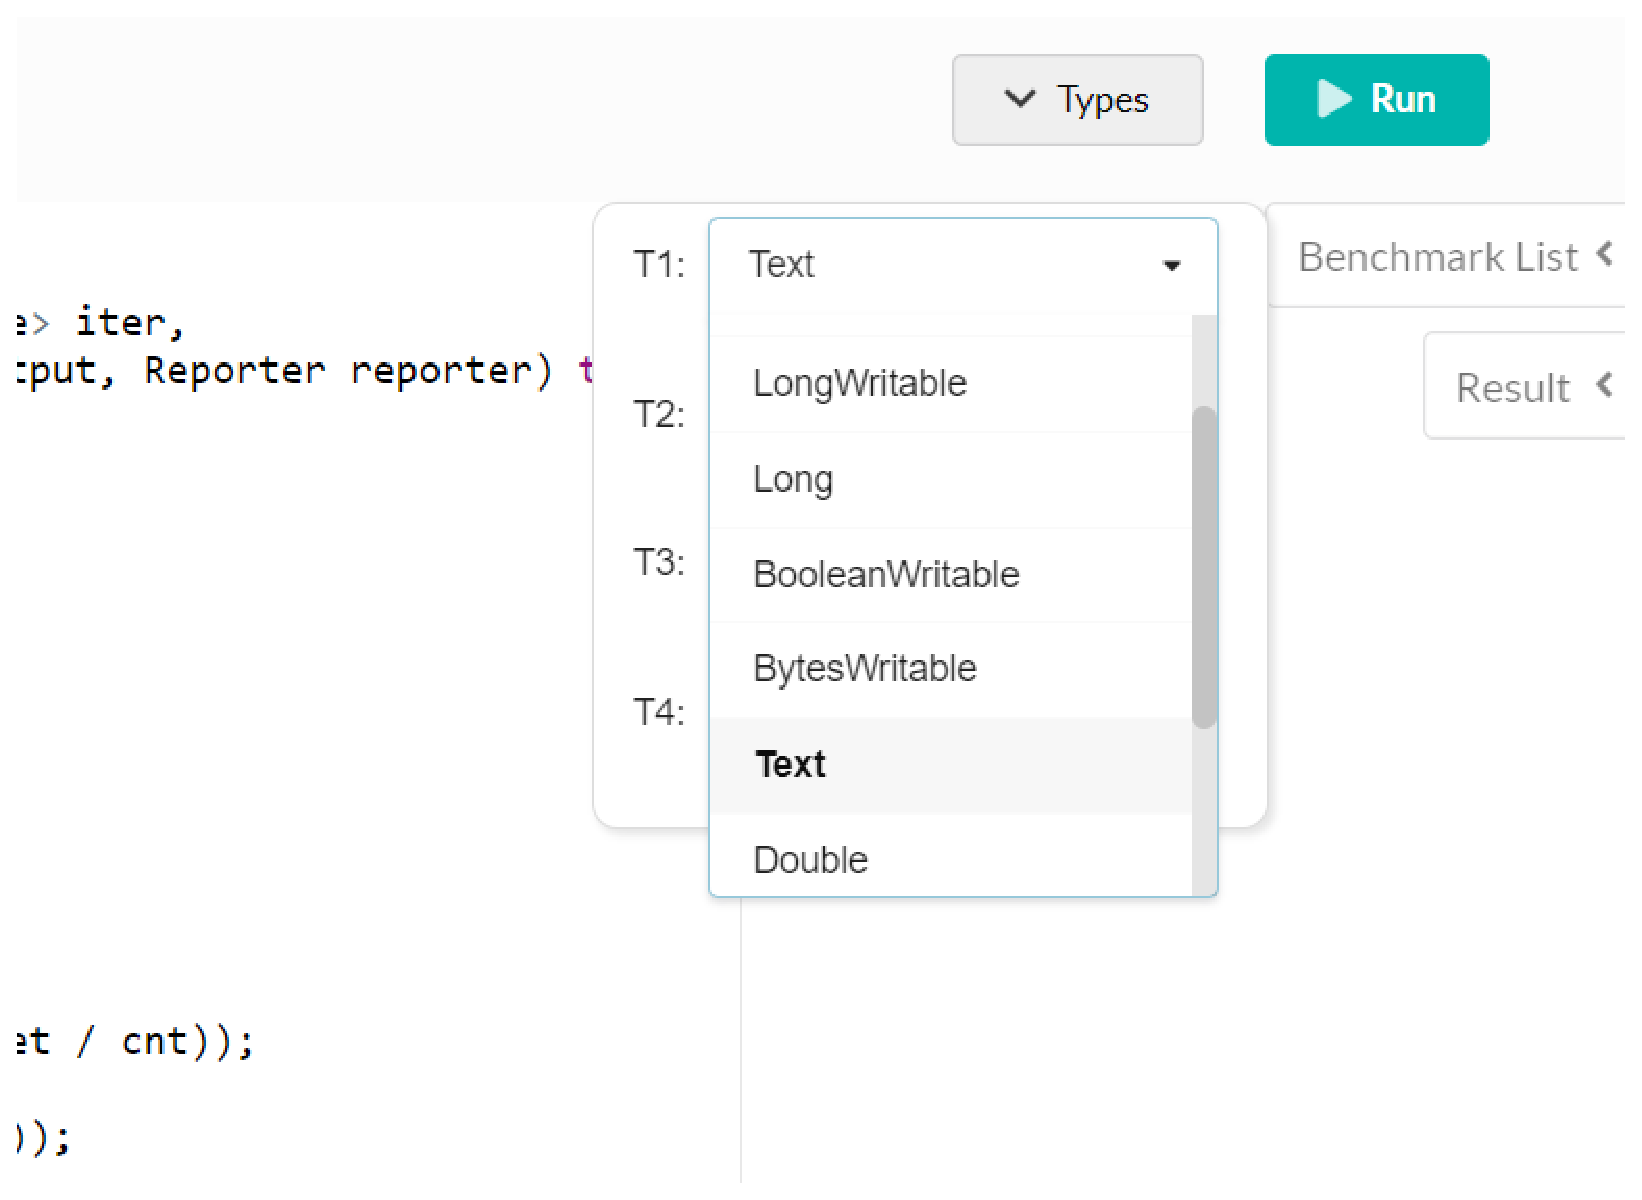
\includegraphics[width=.8\linewidth]{screenshots/selectable_types}
% \vspace{-5pt}
\caption{Selectable types (a part).}
\label{fig:selectable_types}
% \vspace{-15pt}
\end{center}
\end{figure}

After J-ReCoVer finishes the analysis, the \emph{``Result:''} tab of the right
menu will show the result of the analysis, which can be found in
Figure~\ref{fig:analysis_result}. Figure~\ref{fig:analysis_result_text} shows
the complete analysis report of the benchmark \texttt{dis.java} in
Figure~\ref{fig:main_screen}.

\begin{figure}
\begin{center}
% \vspace{-10pt}
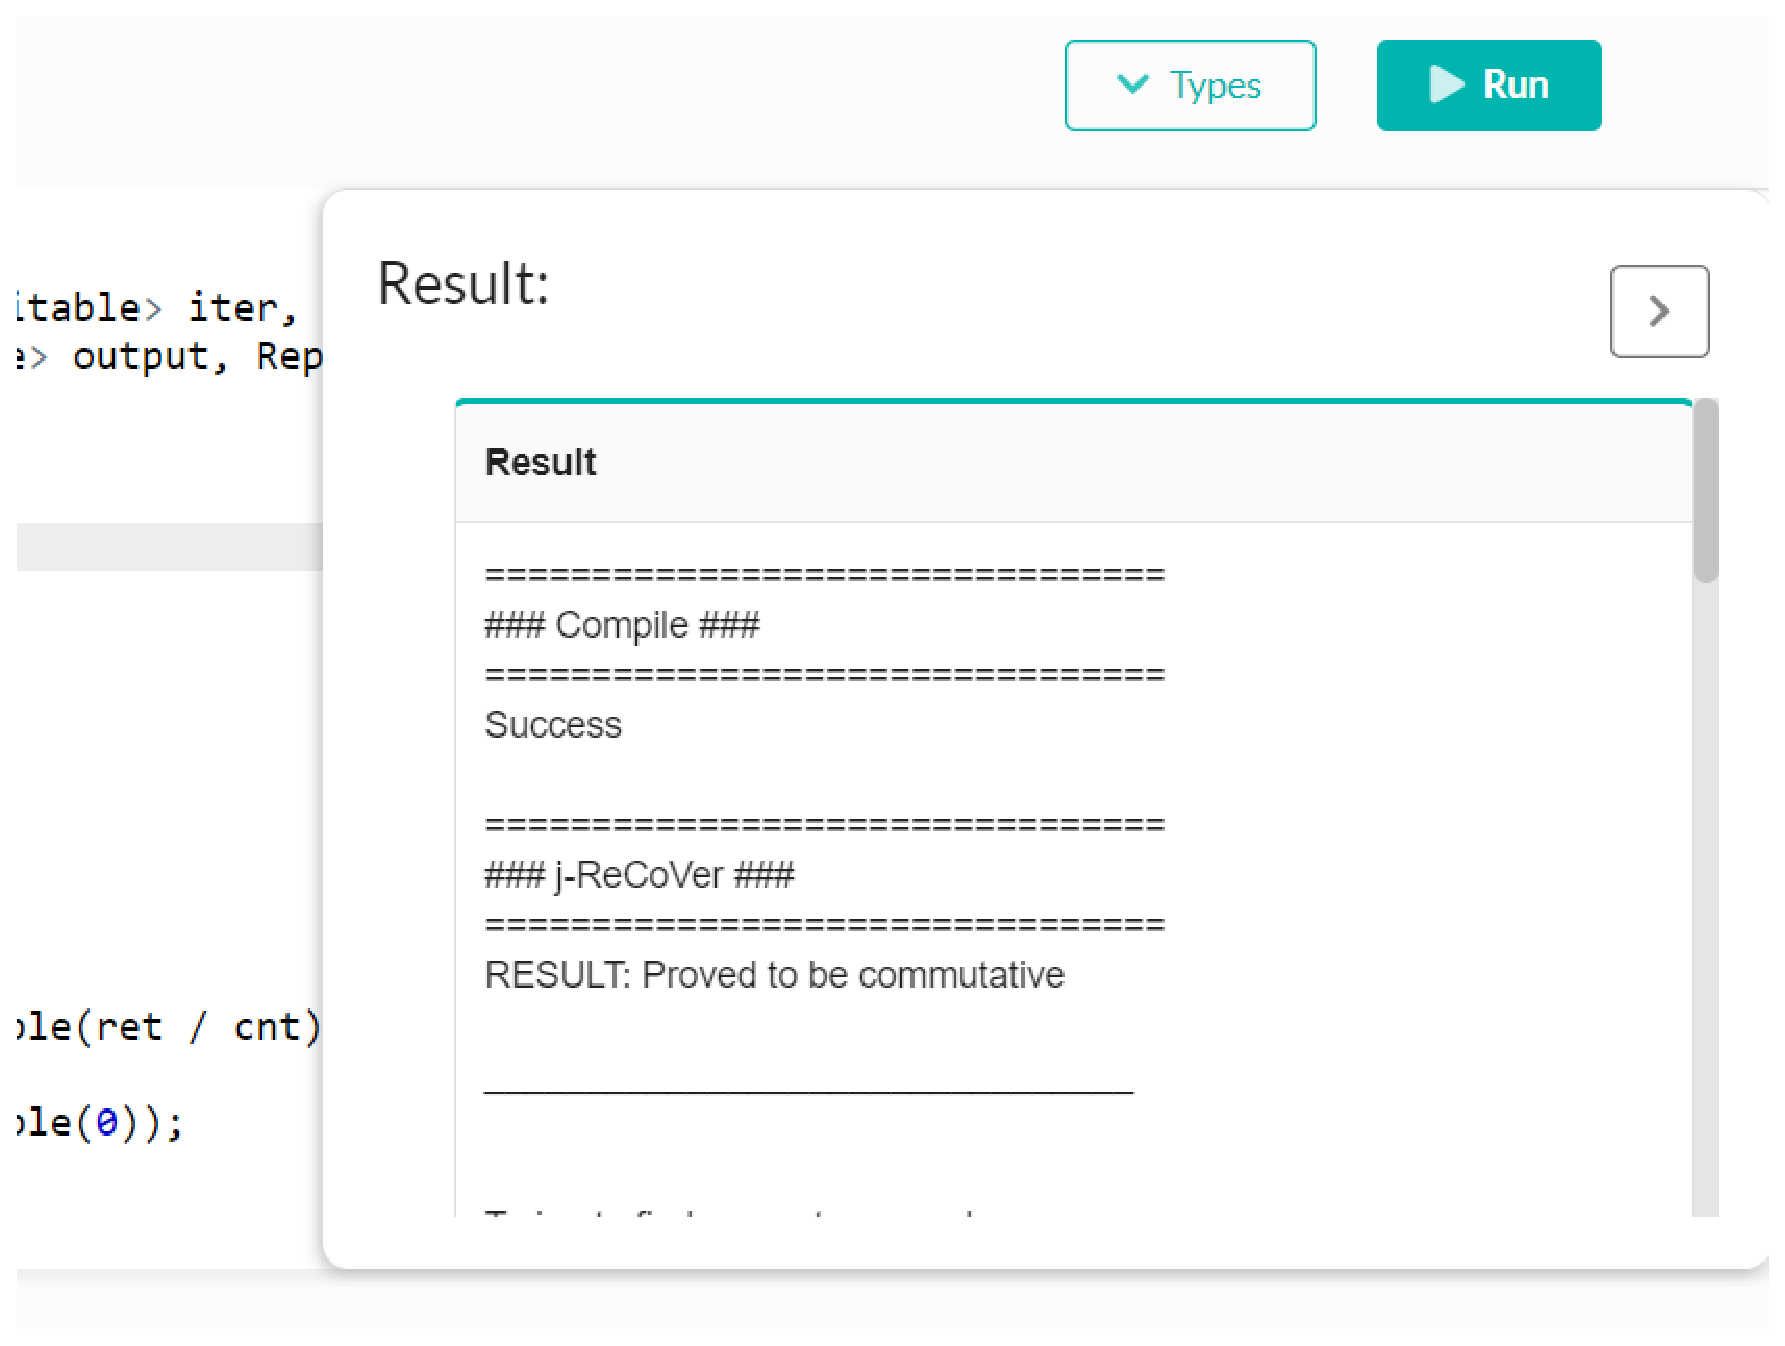
\includegraphics[width=.8\linewidth]{screenshots/analysis_result}
% \vspace{-5pt}
\caption{The analysis result.}
\label{fig:analysis_result}
% \vspace{-15pt}
\end{center}
\end{figure}

\begin{figure}
\begin{center}
\begin{mdframed}[roundcorner=5pt]
\begin{Verbatim}[fontsize=\tiny]
================================
### Compile ###
================================
Success

================================
### j-ReCoVer ###
================================
RESULT: Proved to be commutative

________________________________


Trying to find a counterexample...

RESULT: Cannot find a counterexample in 500 tests
Testcases were generated randomly.

Following are the first 50 lines of testcases:
Input1: o [5, 4, 5, 2, -1]
Input2: o [-1, 4, 5, 5, 2]
Output1: 

Key: [o]
Val: [0.0]
--
Output2: 

Key: [o]
Val: [0.0]
--------
Input1: j [1, -1, 0, 3, -2]
Input2: j [0, 3, -2, 1, -1]
Output1: 

Key: [j]
Val: [0.0]
--
Output2: 

Key: [j]
Val: [0.0]
--------
Input1: e [4, 3, 5, -4, 1]
Input2: e [4, -4, 5, 3, 1]
Output1: 

Key: [e]
Val: [0.0]
--
Output2: 

Key: [e]
Val: [0.0]
--------
Input1: s [3, 0, 2, -4, -1]
Input2: s [3, -1, 0, -4, 2]
Output1: 

Key: [s]
Val: [0.0]
--
Output2: 

Key: [s]
Val: [0.0]
--------
Input1: v [-3, -2, 3, 3, -3]
Input2: v [3, -2, -3, -3, 3]
\end{Verbatim}
\end{mdframed}
\caption{The analysis result of \texttt{dis.java}.}
\label{fig:analysis_result_text}
\end{center}
\end{figure}

When an analysis is started, J-ReCoVer first tries to compile the chosen example
and then performs its commutativity analysis. If the analysis cannot conclude
that the example is commutative, J-ReCoVer then runs 500 randomly generated test
cases to try to find a counterexample. If the test cases all pass, then the
result will be ``unknown''.

\clearpage
\subsection{Run Analysis of a User-defined Reducer Function}
\label{appendix:3}

Besides examples from the benchmark, J-ReCoVer also provides an interactive way
for analysing a user-defined reducer function.  One can directly edit the code
of a selected example in the coding space for further analysis, or write a
reducer function from scratch. The upper-left menu (below the top menu)
provides blank templates for two versions of Hadoop. The templates are shown
below:

\begin{mdframed}[roundcorner=5pt]
\begin{verbatim}
public void reduce(T1 key, Iterator<T2> values,
	OutputCollector<T3,T4> oc1, Reporter reporter)
		throws IOException,InterruptedException {

}
\end{verbatim}
\end{mdframed}

\begin{mdframed}[roundcorner=5pt]
\begin{verbatim}
public void reduce(T1 key, Iterable<T2> values,
	Context context) throws IOException,InterruptedException {

}
\end{verbatim}
\end{mdframed}

In this case, one would have to manually fill the types T1 to T4 and the
function body, and then select the types from the pull-down menu as shown in
Figure~\ref{fig:type_select_menu} and Figure~\ref{fig:selectable_types}. All
selectable types are:

\begin{itemize}
\item Long,
\item BooleanWritable,
\item BytesWritable,
\item Text,
\item Double,
\item DoubleWritable,
\item Float,
\item FloatWritable.
\end{itemize}

\clearpage
\appendix

\section{J-ReCoVer Demo}

Our plan is to demonstrate the basic usage of J-ReCoVer on two examples. The
first example is a reducer that is not commutative, and J-ReCoVer will report a
counterexample. Based on this counterexample, we will fix the reducer to get the
second example, and let J-ReCoVer to check it again. Now, J-ReCoVer will report
that the reducer is commutative. Below, we give a more detailed description of
the functionalities of J-ReCoVer. 

\subsection{The User Interface of J-ReCoVer}
\label{appendix:1}

Figure~\ref{fig:main_screen} shows the main screen of J-ReCoVer. 

\begin{figure}
\begin{center}
% \vspace{-10pt}
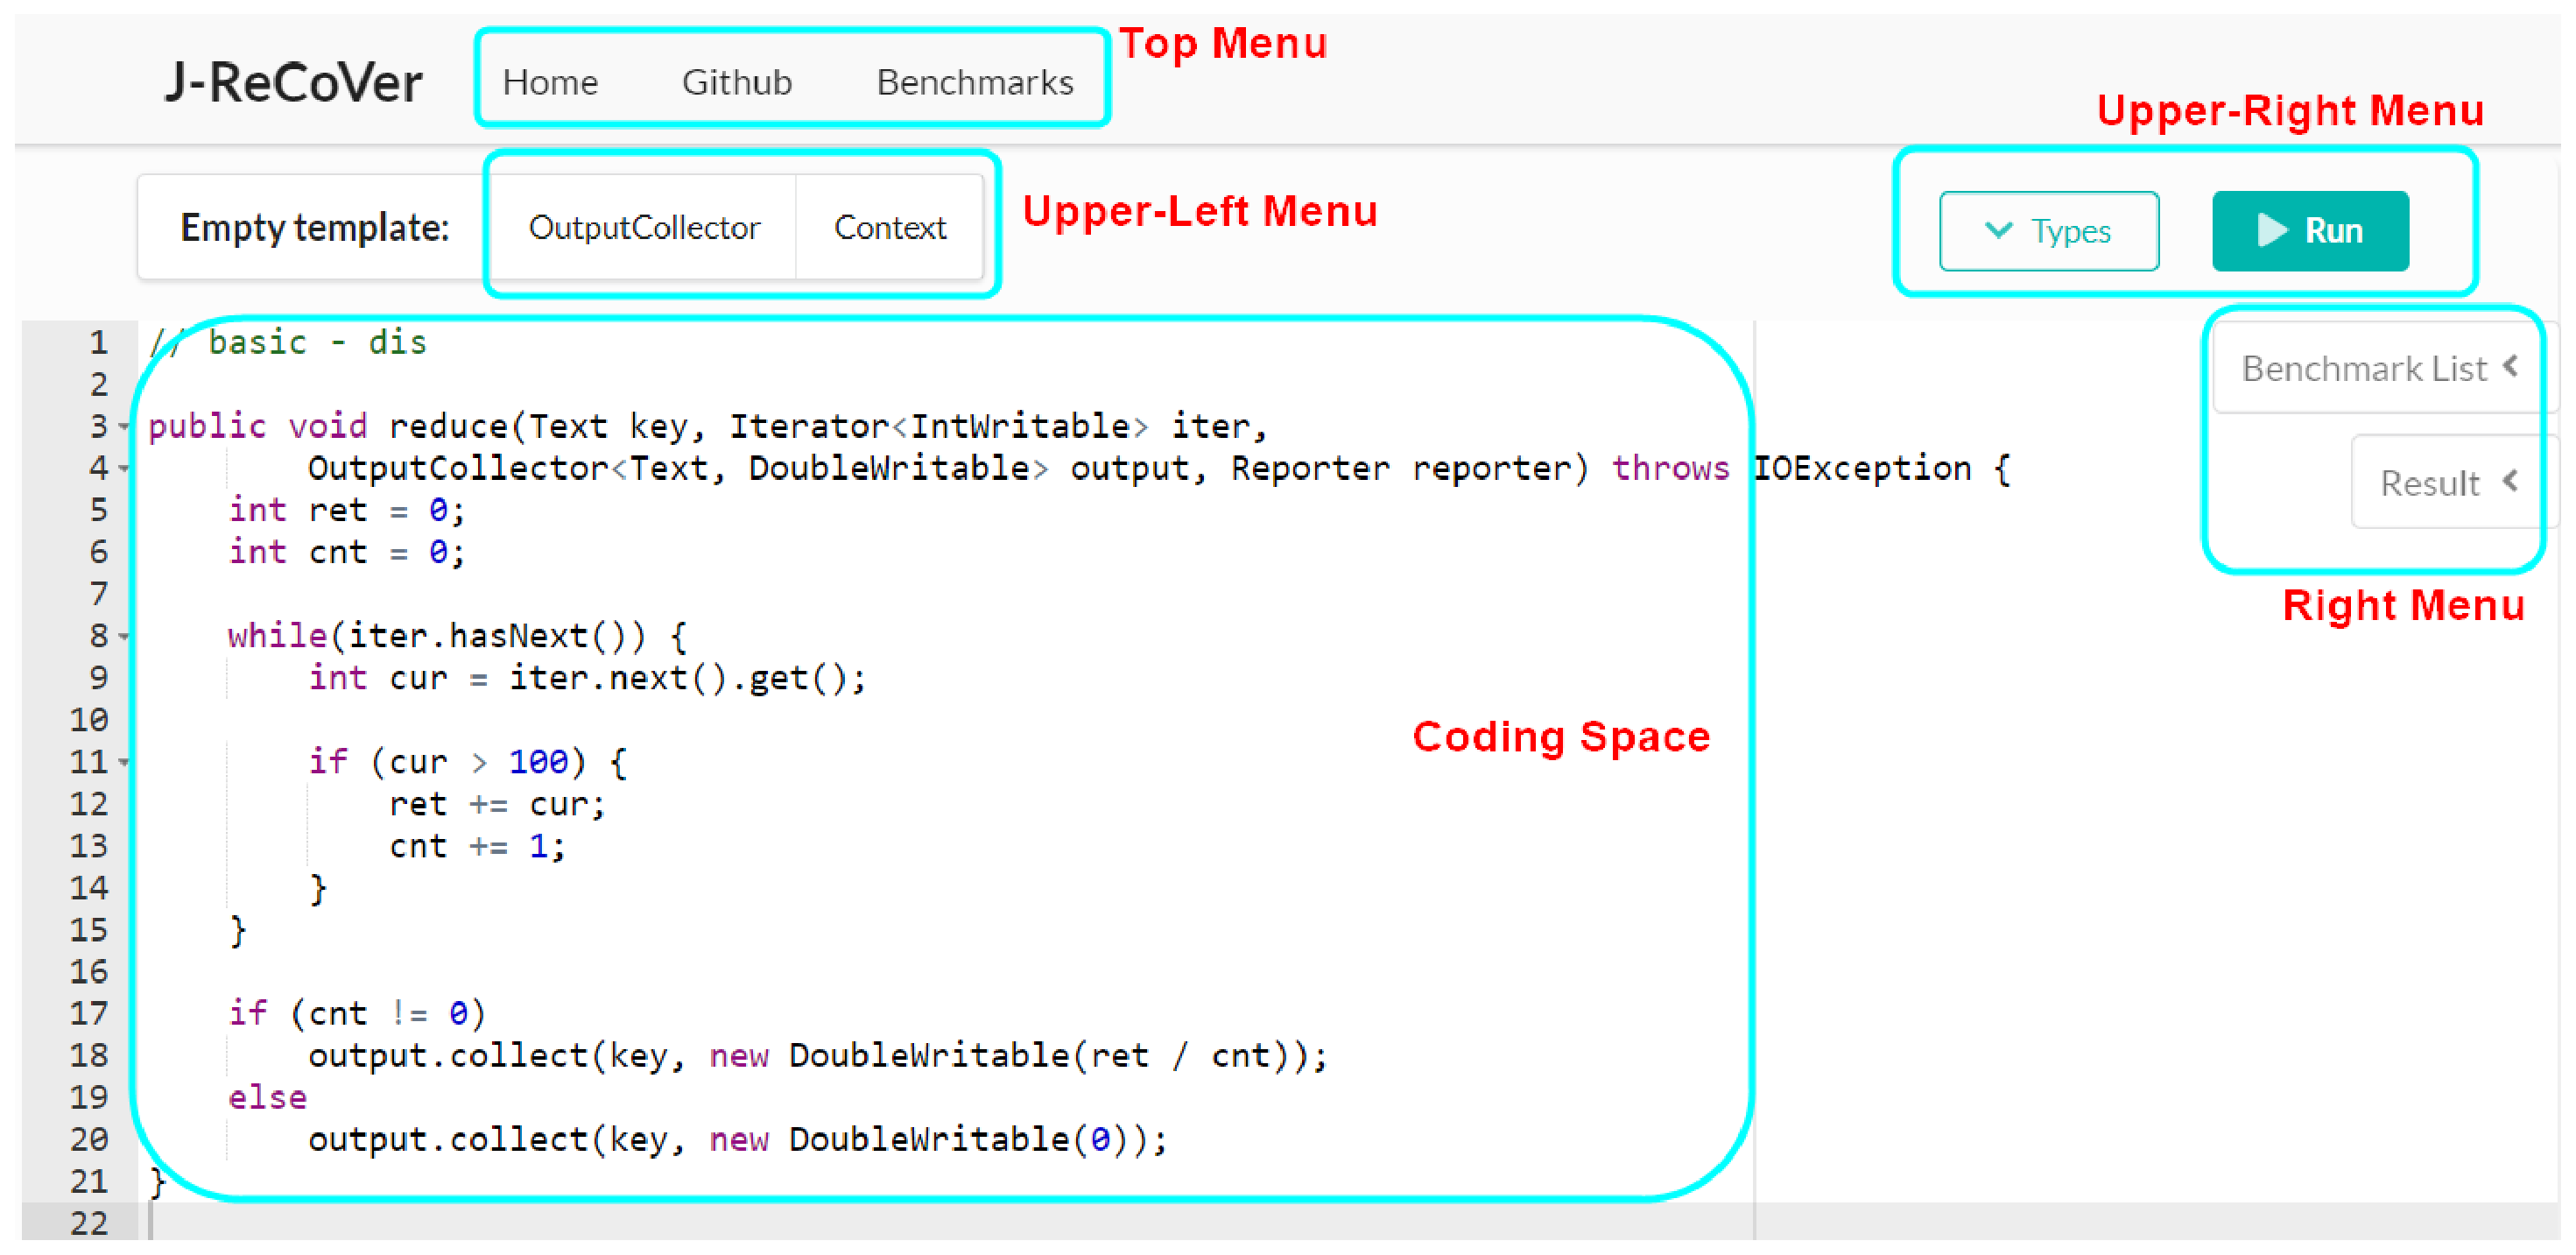
\includegraphics[width=.9\linewidth]{screenshots/main_screen_marked}
% \vspace{-5pt}
\caption{The main screen of J-ReCoVer.}
\label{fig:main_screen}
% \vspace{-15pt}
\end{center}
\end{figure}

The alignment of the user interface elements in the main screen is as follows:
\begin{itemize}
\item
Top Menu:
\begin{itemize}
\item
\emph{``GitHub''} opens a new tab of the repository of J-ReCoVer. The repository
does also contain the source code of our benchmarks.
\item
\emph{``Benchmark''} leads to the list of benchmarks we collected with their
results of commutativity analysis as Fig.~\ref{fig:benchmark_list} shows. Select
a file name or use the ``try it'' button to select an example and go back to the main screen.
\end{itemize}
\item
Right Menu:
\begin{itemize}
\item
\emph{``Benchmark List''} provides a quick selection of examples in the
benchmark (Fig.~\ref{fig:benchmark_list_right}).
\item
\emph{``Results''} shows the last analysis result.
\end{itemize}
\item
Upper-Right Menu:
\begin{itemize}
\item
\emph{``Type''} provides types that J-ReCoVer supports. Details are explained in
Appendix~\ref{appendix:3}.
\item
\emph{``Run''} starts the analysis of the selected example.
\end{itemize}
\item
Upper-Left Menu: See Appendix~\ref{appendix:3}.
\item
Coding Space.
\end{itemize}

\begin{figure}
\begin{center}
% \vspace{-10pt}
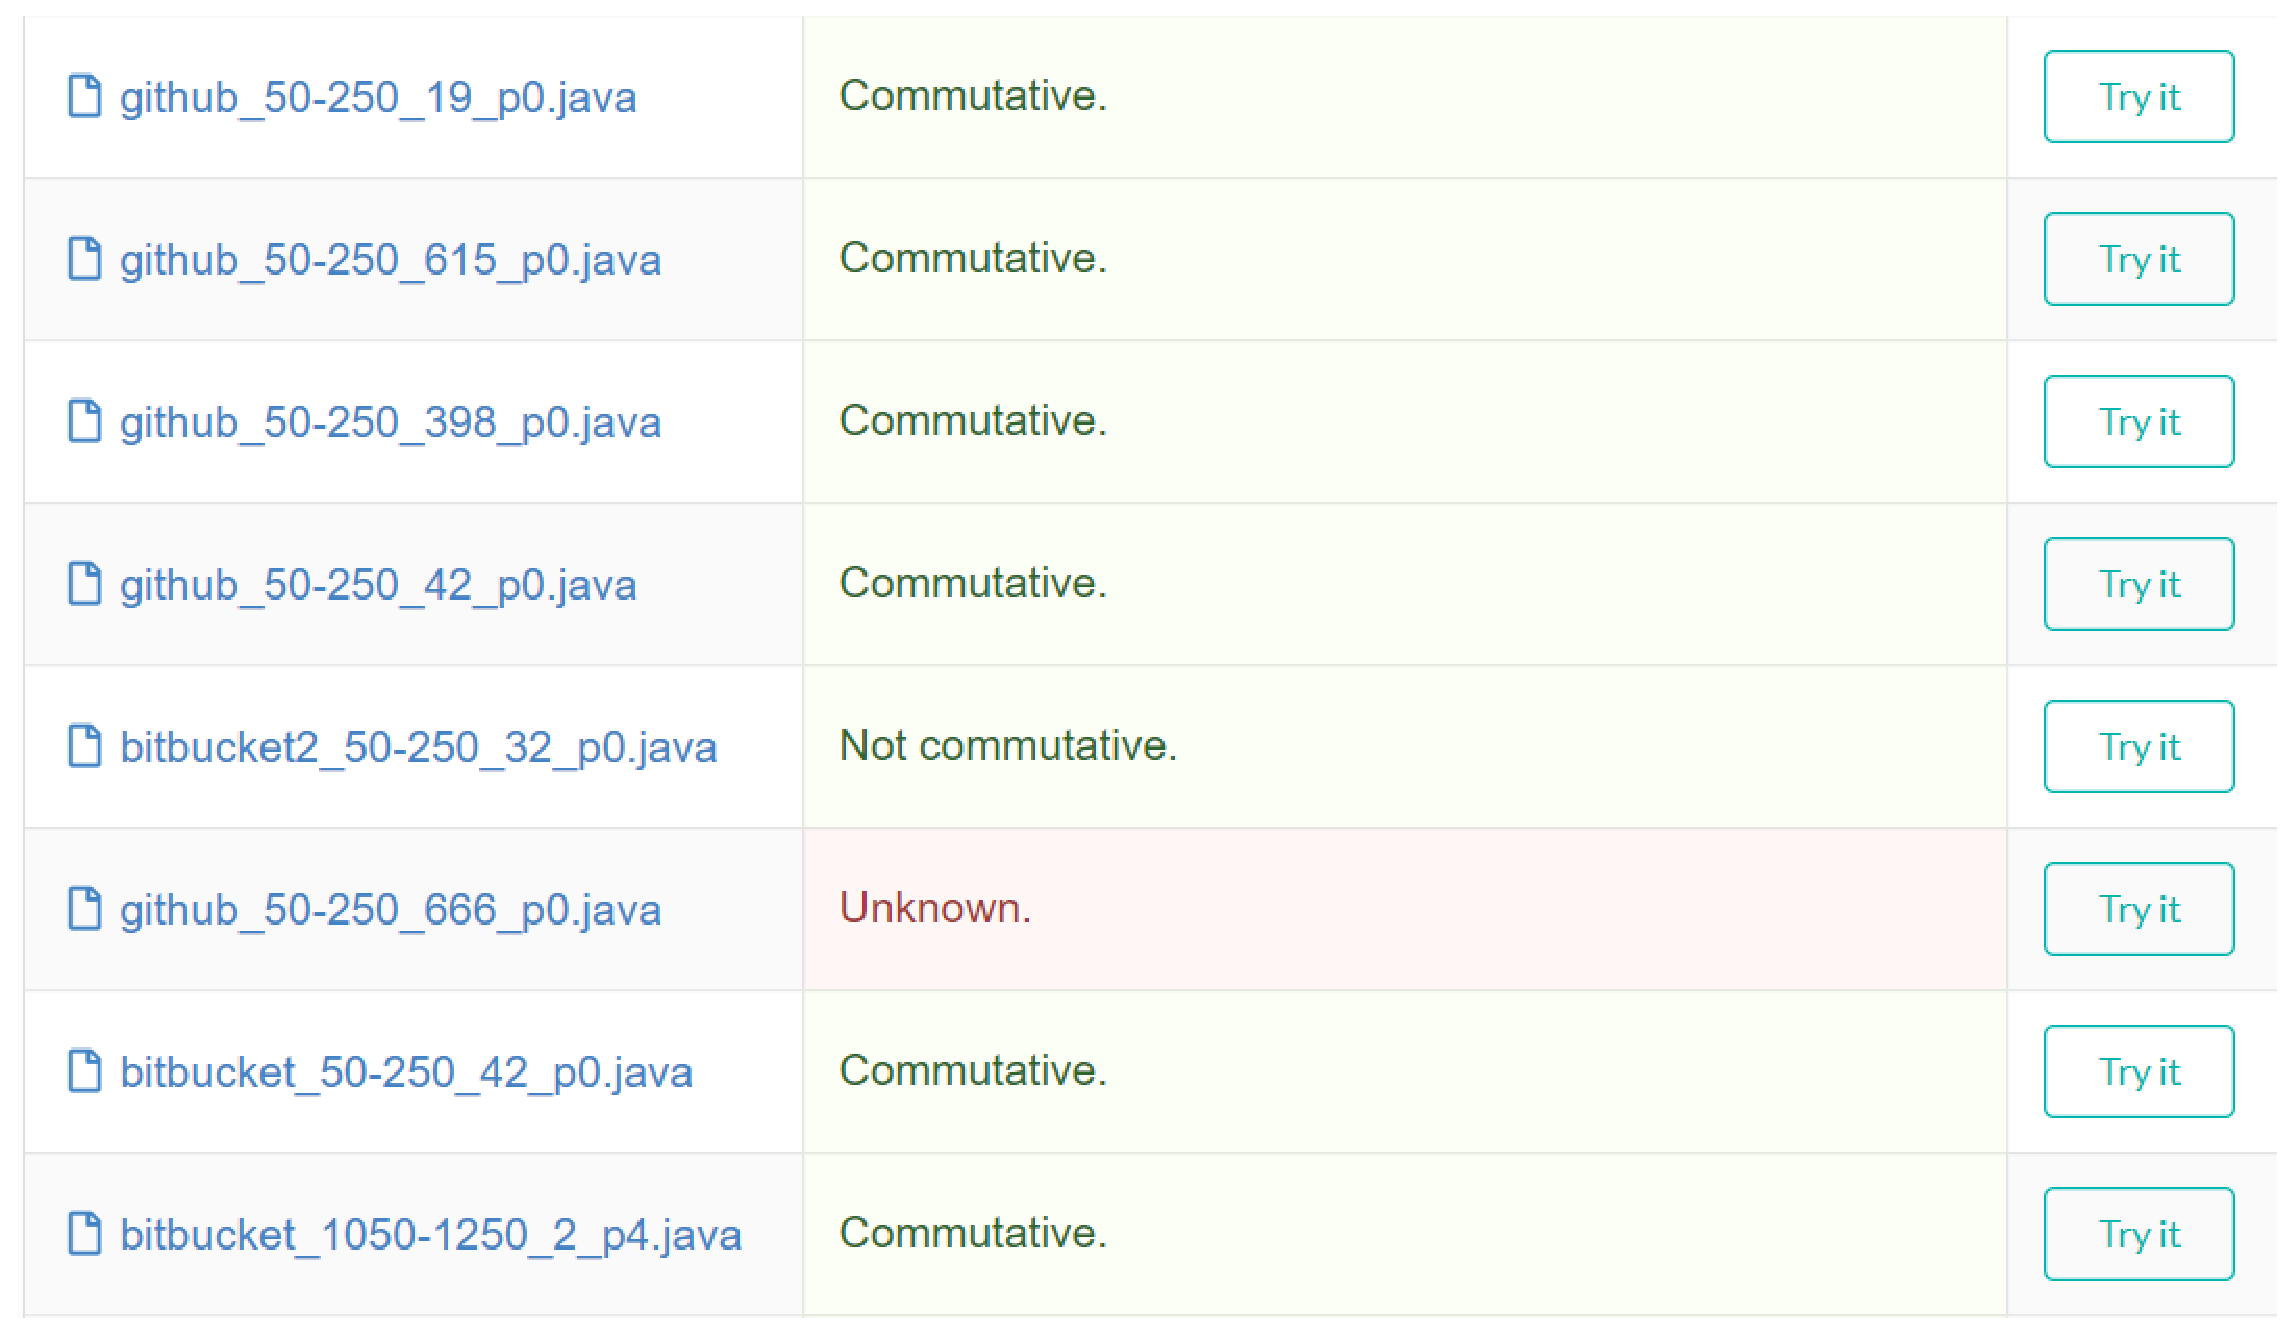
\includegraphics[width=.8\linewidth]{screenshots/benchmark_list}
% \vspace{-5pt}
\caption{A benchmark list from the top menu (a part).}
\label{fig:benchmark_list}
% \vspace{-15pt}
\end{center}
\end{figure}

\begin{figure}
\begin{center}
% \vspace{-10pt}
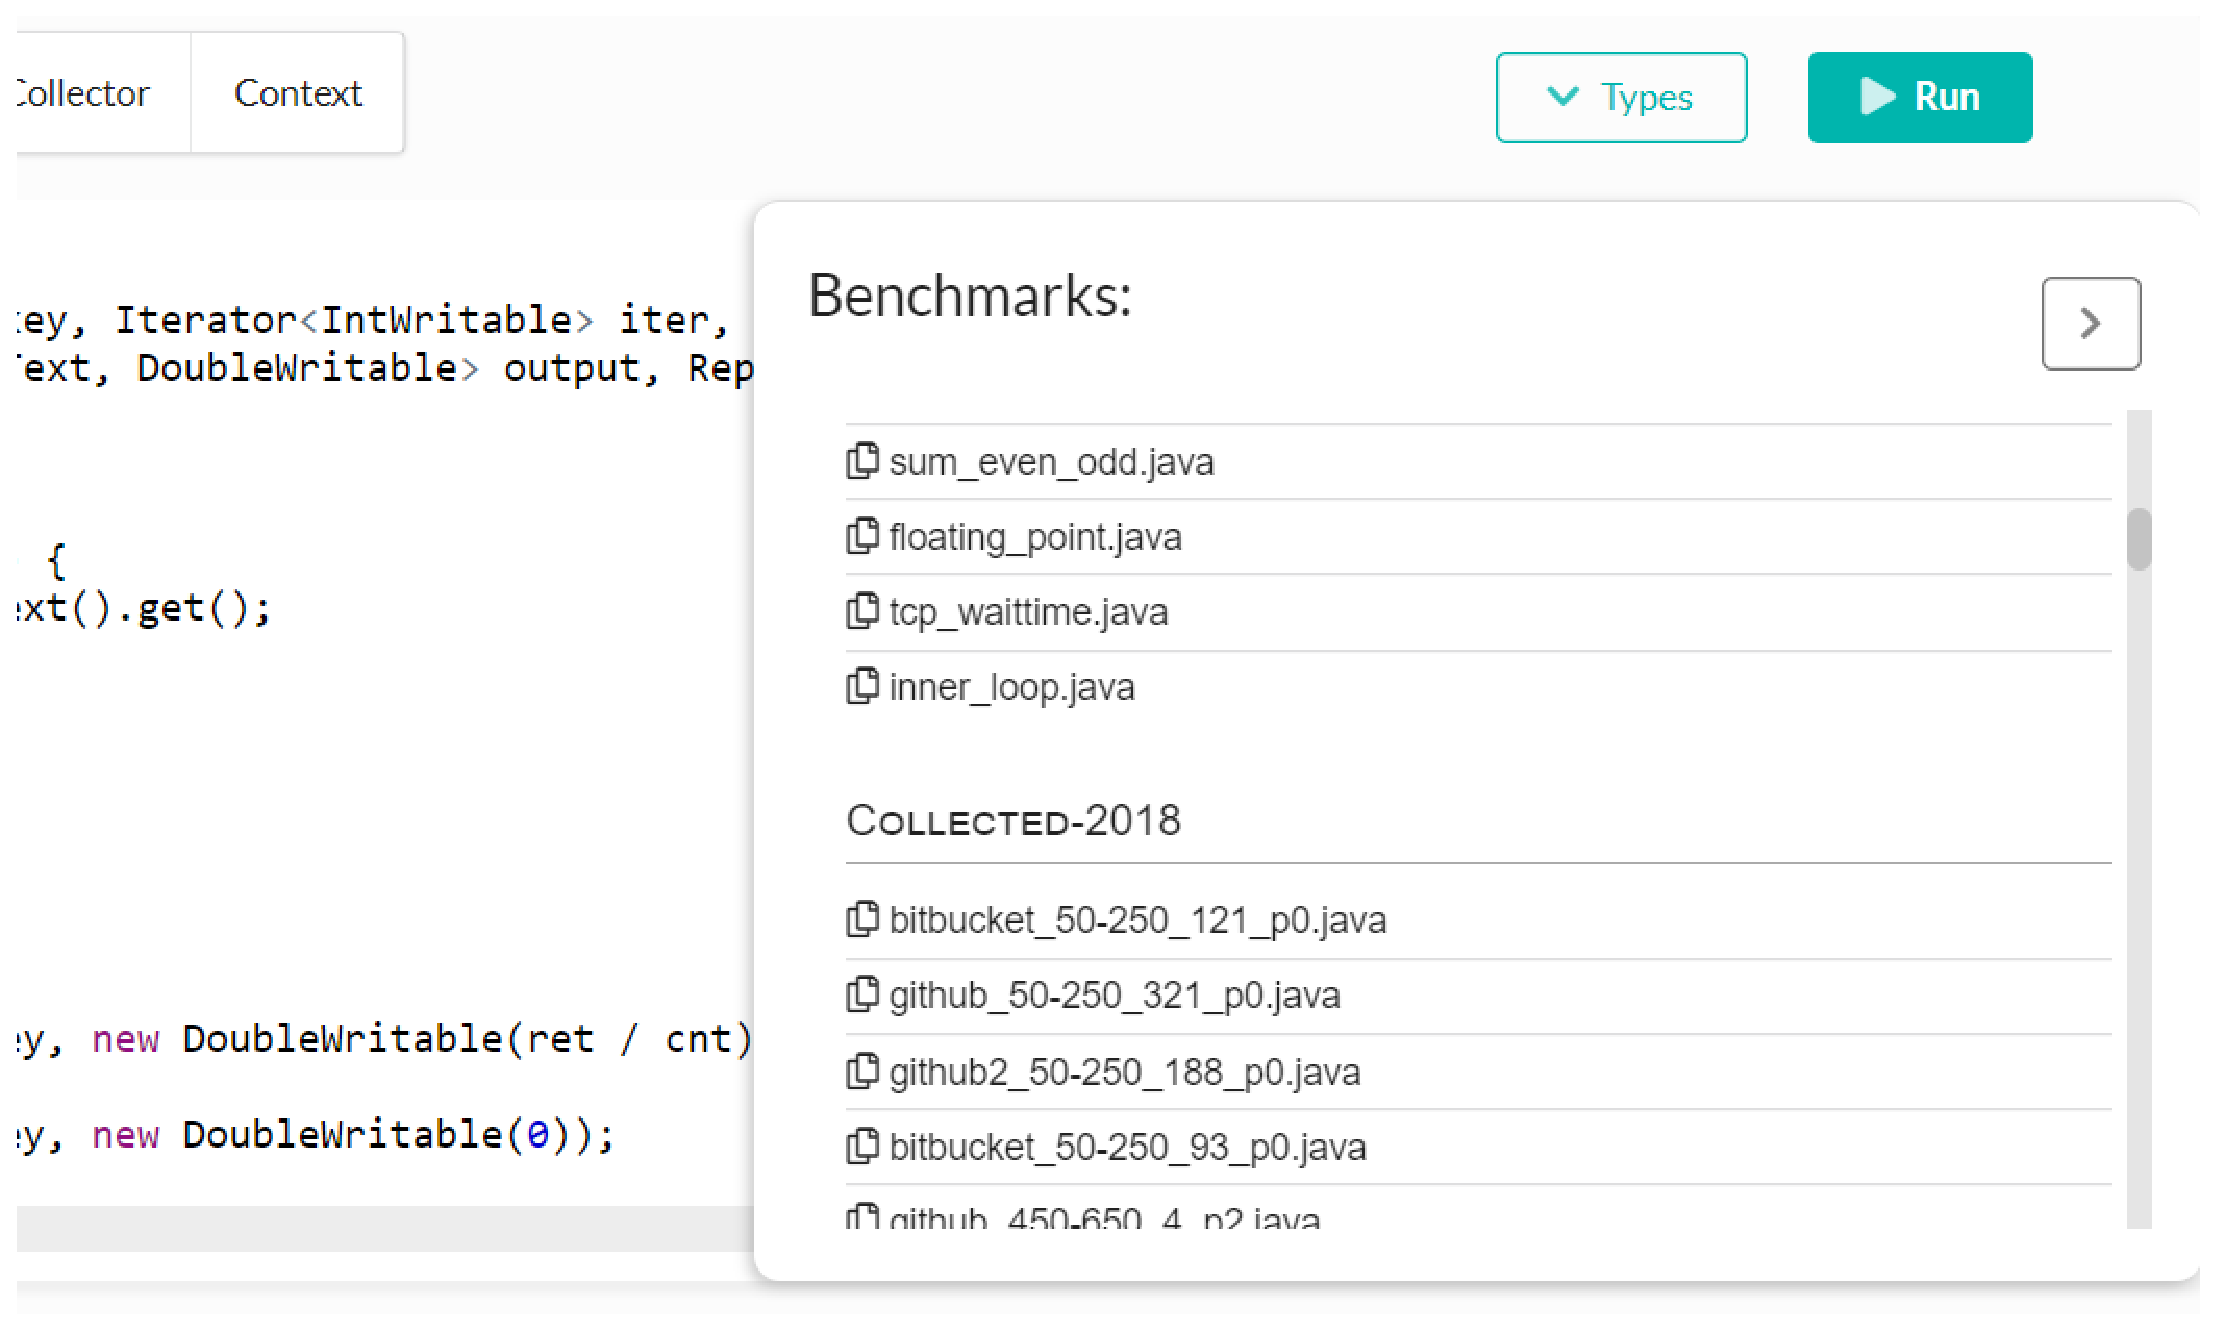
\includegraphics[width=.8\linewidth]{screenshots/benchmark_list_right}
% \vspace{-5pt}
\caption{A benchmark list from the right menu (a part).}
\label{fig:benchmark_list_right}
% \vspace{-15pt}
\end{center}
\end{figure}

\subsection{Run Analysis of a Selected Benchmark Example}
\label{appendix:2}

To run the analysis, one can choose an example from the benchmark using either
the top menu or the right menu and then click the ``Run'' button of the
upper-right menu to start the commutativity analysis of the selected example.
The pull-down menu ``Types'' of the upper-right menu provides selectable types
for input \texttt{(T1,T2)} and output \texttt{(T3,T4)} key-value pairs.
Fig.~\ref{fig:type_select_menu} shows the pull-down menu and
Fig.~\ref{fig:selectable_types} shows a part of the selectable types in
J-ReCoVer.  If one selects an example from the benchmark, the types will be
automatically selected to match the example. The selection will be needed if the
user wants to write a reduce function for analysis  from scratch (see
Appendix~\ref{appendix:3}).

\begin{figure}
\begin{center}
% \vspace{-10pt}
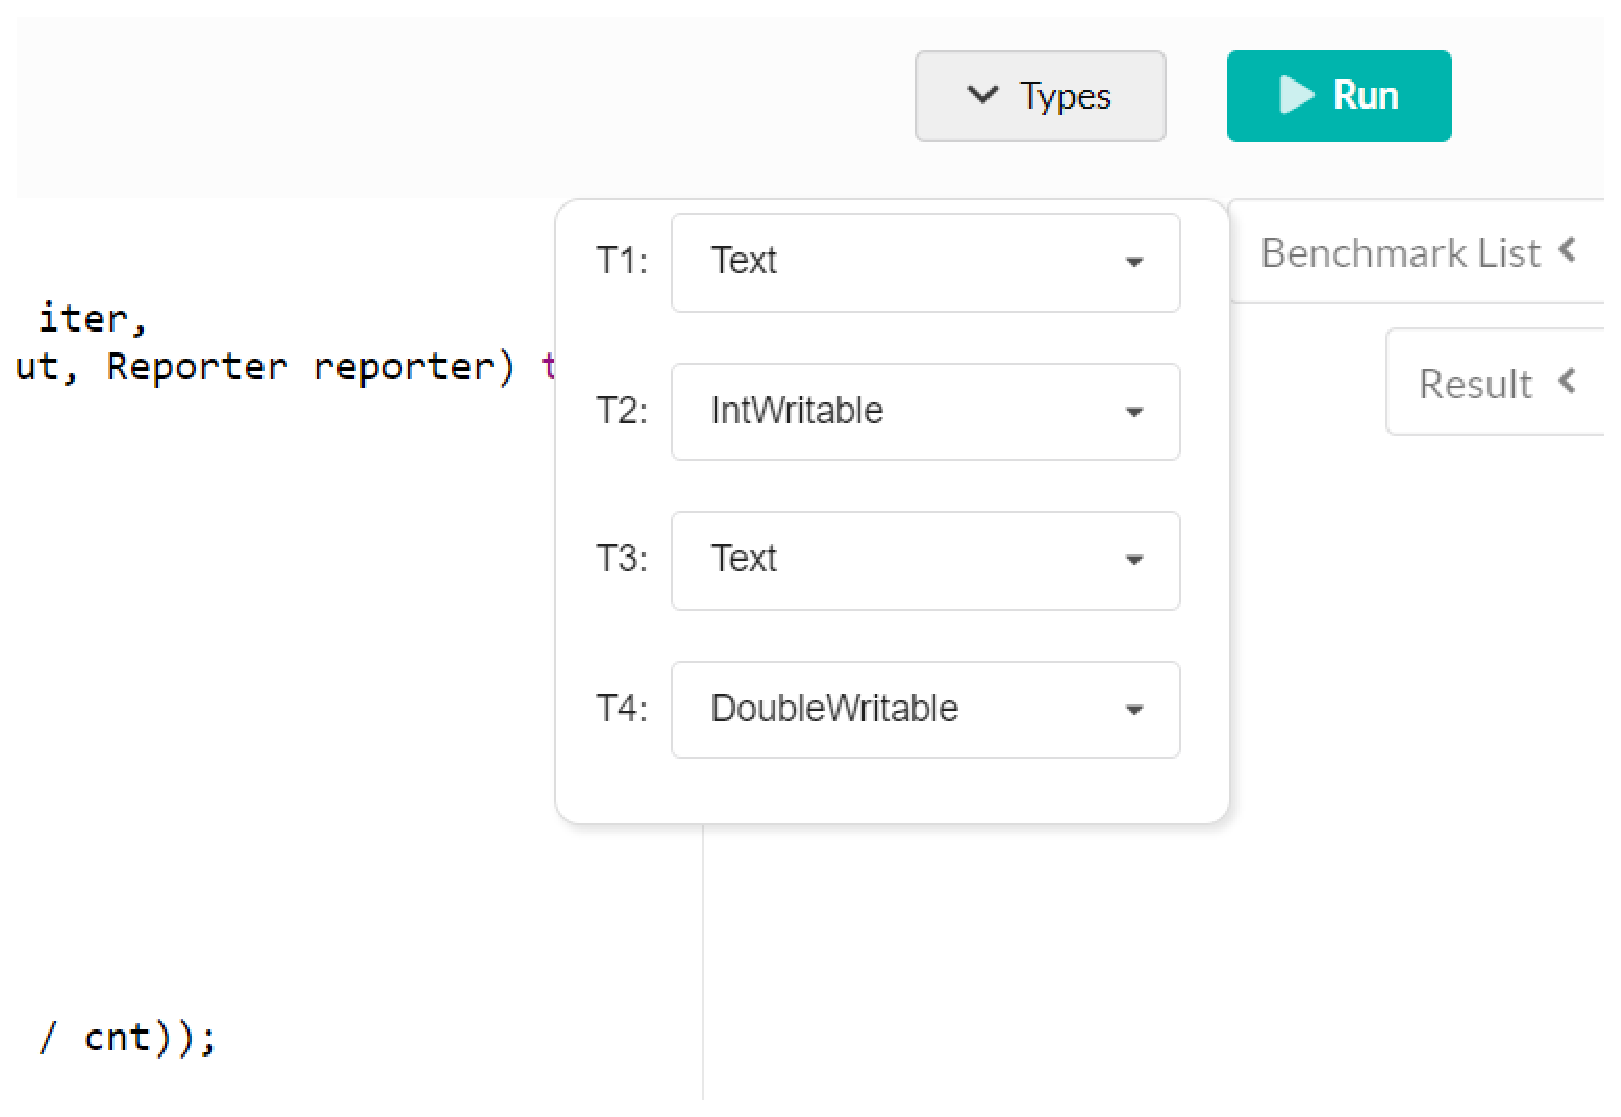
\includegraphics[width=.8\linewidth]{screenshots/type_select_menu}
% \vspace{-5pt}
\caption{The type selection menu.}
\label{fig:type_select_menu}
% \vspace{-15pt}
\end{center}
\end{figure}

\begin{figure}
\begin{center}
% \vspace{-10pt}
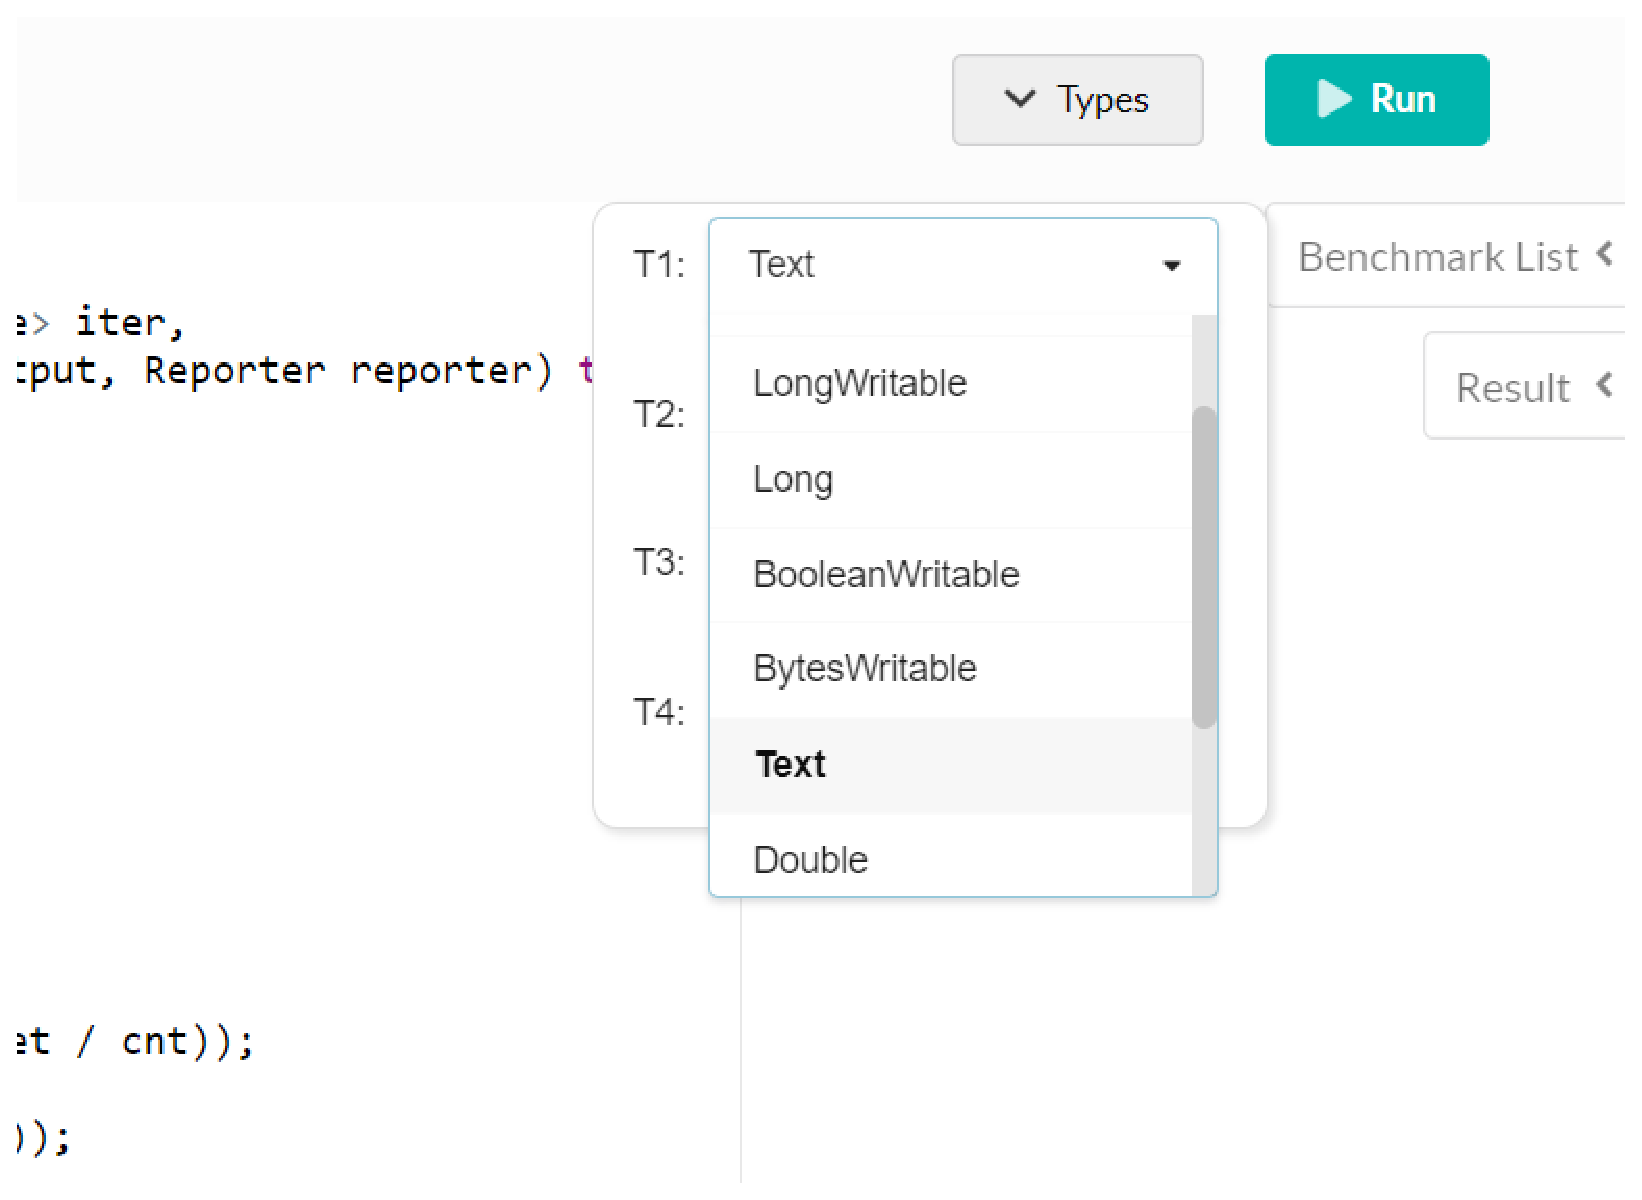
\includegraphics[width=.8\linewidth]{screenshots/selectable_types}
% \vspace{-5pt}
\caption{Selectable types (a part).}
\label{fig:selectable_types}
% \vspace{-15pt}
\end{center}
\end{figure}

After J-ReCoVer finishes the analysis, the \emph{``Result:''} tab of the right
menu will show the result of the analysis, which can be found in
Figure~\ref{fig:analysis_result}. Figure~\ref{fig:analysis_result_text} shows
the complete analysis report of the benchmark \texttt{dis.java} in
Figure~\ref{fig:main_screen}.

\begin{figure}
\begin{center}
% \vspace{-10pt}
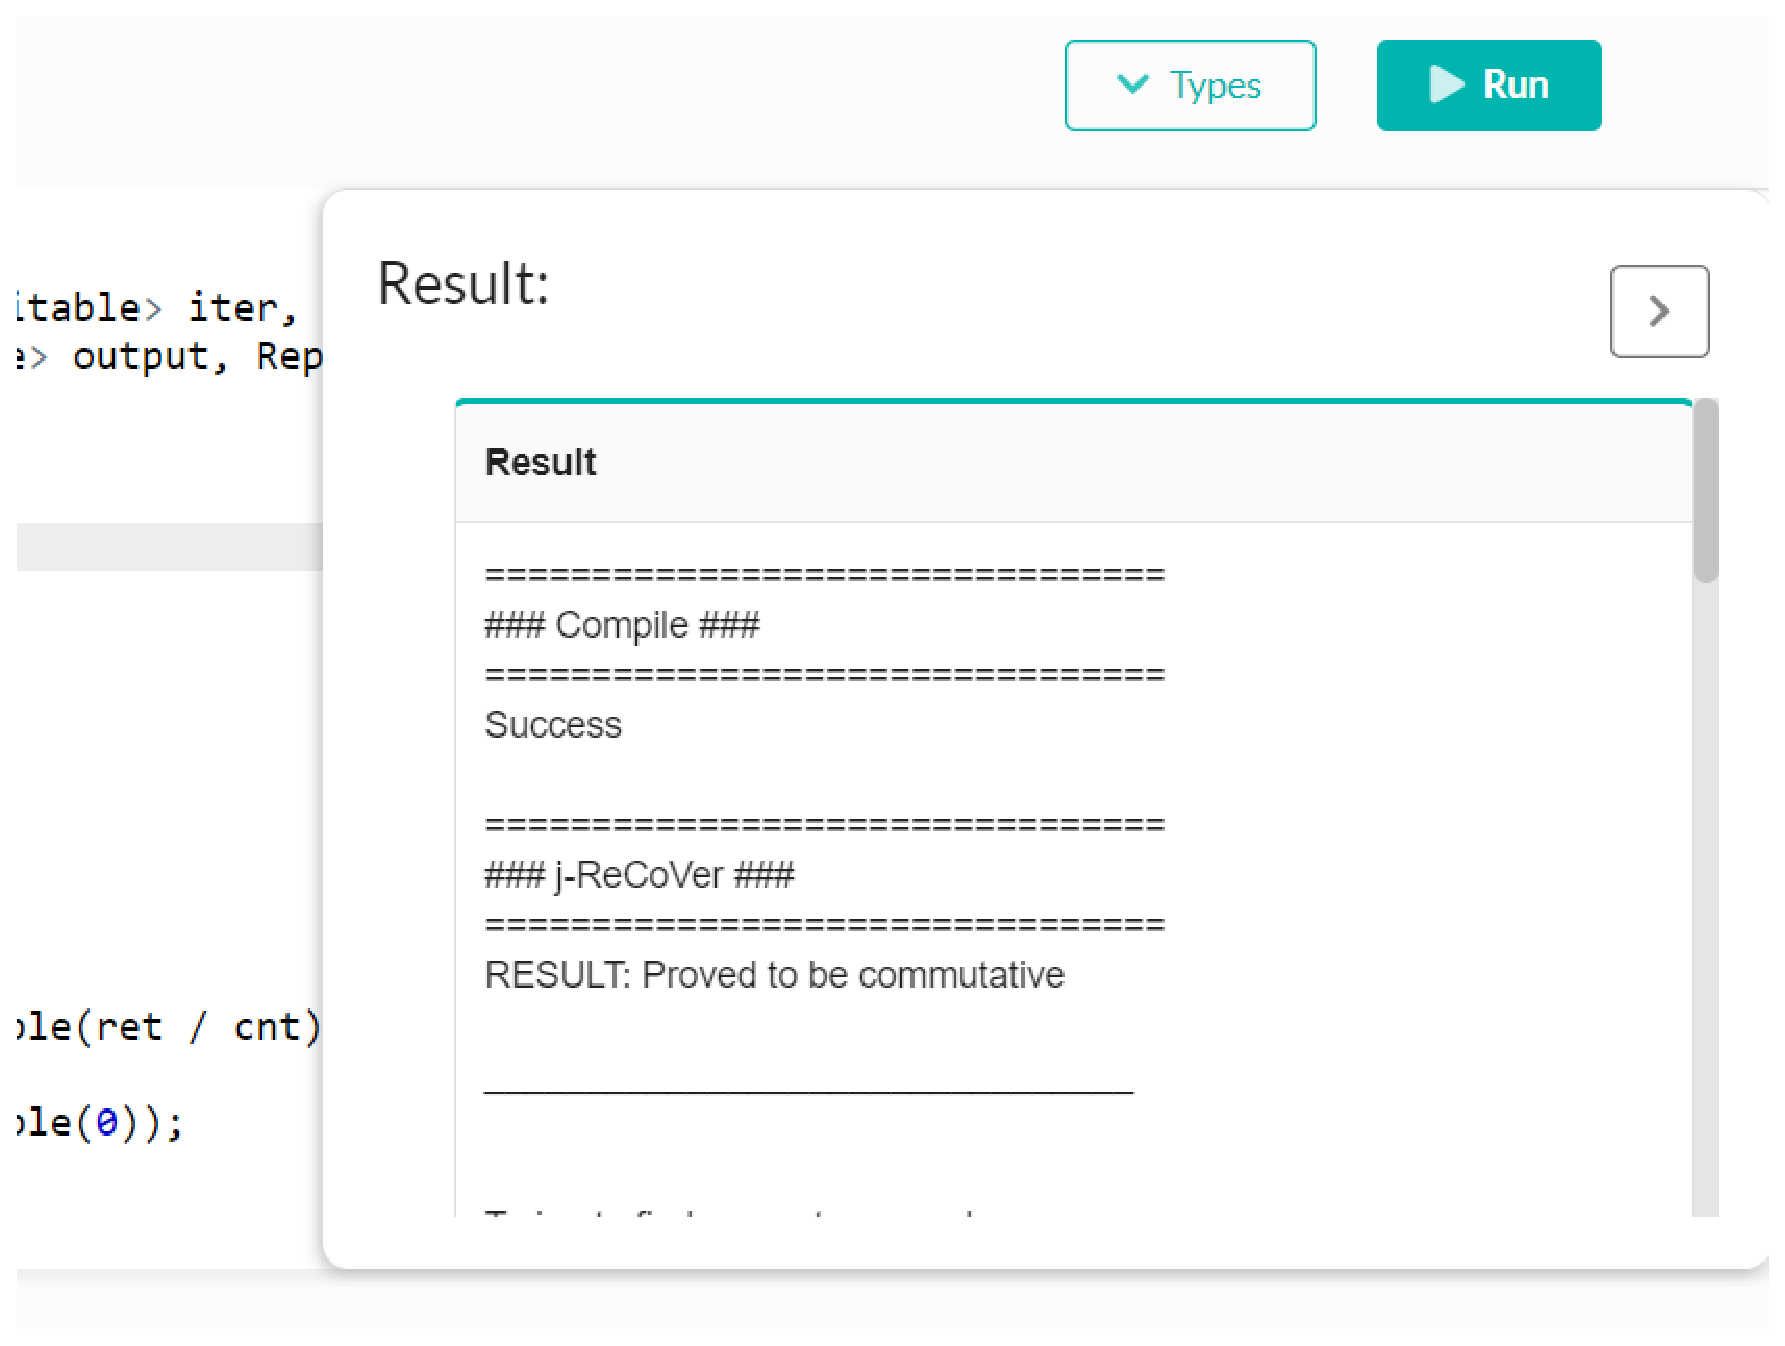
\includegraphics[width=.8\linewidth]{screenshots/analysis_result}
% \vspace{-5pt}
\caption{The analysis result.}
\label{fig:analysis_result}
% \vspace{-15pt}
\end{center}
\end{figure}

\begin{figure}
\begin{center}
\begin{mdframed}[roundcorner=5pt]
\begin{Verbatim}[fontsize=\tiny]
================================
### Compile ###
================================
Success

================================
### j-ReCoVer ###
================================
RESULT: Proved to be commutative

________________________________


Trying to find a counterexample...

RESULT: Cannot find a counterexample in 500 tests
Testcases were generated randomly.

Following are the first 50 lines of testcases:
Input1: o [5, 4, 5, 2, -1]
Input2: o [-1, 4, 5, 5, 2]
Output1: 

Key: [o]
Val: [0.0]
--
Output2: 

Key: [o]
Val: [0.0]
--------
Input1: j [1, -1, 0, 3, -2]
Input2: j [0, 3, -2, 1, -1]
Output1: 

Key: [j]
Val: [0.0]
--
Output2: 

Key: [j]
Val: [0.0]
--------
Input1: e [4, 3, 5, -4, 1]
Input2: e [4, -4, 5, 3, 1]
Output1: 

Key: [e]
Val: [0.0]
--
Output2: 

Key: [e]
Val: [0.0]
--------
Input1: s [3, 0, 2, -4, -1]
Input2: s [3, -1, 0, -4, 2]
Output1: 

Key: [s]
Val: [0.0]
--
Output2: 

Key: [s]
Val: [0.0]
--------
Input1: v [-3, -2, 3, 3, -3]
Input2: v [3, -2, -3, -3, 3]
\end{Verbatim}
\end{mdframed}
\caption{The analysis result of \texttt{dis.java}.}
\label{fig:analysis_result_text}
\end{center}
\end{figure}

When an analysis is started, J-ReCoVer first tries to compile the chosen example
and then performs its commutativity analysis. If the analysis cannot conclude
that the example is commutative, J-ReCoVer then runs 500 randomly generated test
cases to try to find a counterexample. If the test cases all pass, then the
result will be ``unknown''.

\clearpage
\subsection{Run Analysis of a User-defined Reducer Function}
\label{appendix:3}

Besides examples from the benchmark, J-ReCoVer also provides an interactive way
for analysing a user-defined reducer function.  One can directly edit the code
of a selected example in the coding space for further analysis, or write a
reducer function from scratch. The upper-left menu (below the top menu)
provides blank templates for two versions of Hadoop. The templates are shown
below:

\begin{mdframed}[roundcorner=5pt]
\begin{verbatim}
public void reduce(T1 key, Iterator<T2> values,
	OutputCollector<T3,T4> oc1, Reporter reporter)
		throws IOException,InterruptedException {

}
\end{verbatim}
\end{mdframed}

\begin{mdframed}[roundcorner=5pt]
\begin{verbatim}
public void reduce(T1 key, Iterable<T2> values,
	Context context) throws IOException,InterruptedException {

}
\end{verbatim}
\end{mdframed}

In this case, one would have to manually fill the types T1 to T4 and the
function body, and then select the types from the pull-down menu as shown in
Figure~\ref{fig:type_select_menu} and Figure~\ref{fig:selectable_types}. All
selectable types are:

\begin{itemize}
\item Long,
\item BooleanWritable,
\item BytesWritable,
\item Text,
\item Double,
\item DoubleWritable,
\item Float,
\item FloatWritable.
\end{itemize}


%%%%%%%%%%%%%%%%%%%%%%%%%%%%%%%%%%%%%%%%%%%%%%%%%%%%%%%%%%%%%%%%%%%%%%%%%%%%%%
\end{document}
%%%%%%%%%%%%%%%%%%%%%%%%%%%%%%%%%%%%%%%%%%%%%%%%%%%%%%%%%%%%%%%%%%%%%%%%%%%%%%
